\documentclass[a4paper, twoside]{book}
\usepackage[T1]{fontenc}
\usepackage[utf8]{inputenc}
\usepackage[italian]{babel}
\usepackage{amsmath, amssymb, amsthm}
\usepackage{geometry}
\usepackage{titling}
\usepackage{enumitem}
\usepackage{pdfpages}
\usepackage{graphicx, float}
\usepackage{subcaption}
\usepackage{caption}
\usepackage{hyperref}
\usepackage{mdframed} % Pacchetto per le cornici
\usepackage{xcolor}   % Pacchetto per la gestione dei colori
\usepackage{forest} %diagrammi ad albero

% Colore per il background delle cornici
\definecolor{grey245}{RGB}{245,245,245}

% Teoremi e definizioni
\theoremstyle{plain}
\newtheorem{theorem}{\textsc{Teorema}}[chapter] 
\newtheorem{lemma}[theorem]{\textsc{Lemma}}
\newtheorem{corollary}[theorem]{\textsc{Corollario}}
\newtheorem{proposition}[theorem]{\textsc{Proposizione}}

\theoremstyle{definition}
\newtheorem{definition}{\textsc{Definizione}}[chapter]  
\newtheorem{example}{\textsc{Esempio}}[chapter] 


%Cornice teorema
\newmdenv[skipabove=5pt,
skipbelow=5pt,
rightline=false,
leftline=true,
topline=false,
bottomline=false,
linecolor=purple,
backgroundcolor=purple!0,
innerleftmargin=5pt,
innerrightmargin=5pt,
innertopmargin=0pt,
innerbottommargin=2pt,
leftmargin=0cm,
rightmargin=0cm,
linewidth=2pt,
splitbottomskip=0pt]{theoremBox}


%Cornice definizione
\newmdenv[skipabove=5pt,
skipbelow=5pt,
rightline=false,
leftline=true,
topline=false,
bottomline=false,
linecolor=blue,
backgroundcolor=blue!0,
innerleftmargin=5pt,
innerrightmargin=5pt,
innertopmargin=0pt,
leftmargin=0cm,
rightmargin=0cm,
linewidth=2pt,
innerbottommargin=2pt]{definitionBox}

%Cornice proposizione
\newmdenv[skipabove=5pt,
skipbelow=5pt,
rightline=false,
leftline=true,
topline=false,
bottomline=false,
linecolor=teal,
backgroundcolor=teal!0,
innerleftmargin=5pt,
innerrightmargin=5pt,
innertopmargin=0pt,
leftmargin=0cm,
rightmargin=0cm,
linewidth=2pt,
innerbottommargin=2pt]{propositionBox}

%Cornice lemma
\newmdenv[skipabove=5pt,
skipbelow=5pt,
rightline=false,
leftline=true,
topline=false,
bottomline=false,
linecolor=orange,
backgroundcolor=orange!0,
innerleftmargin=5pt,
innerrightmargin=5pt,
innertopmargin=0pt,
leftmargin=0cm,
rightmargin=0cm,
linewidth=2pt,
innerbottommargin=2pt]{lemmaBox}

%Cornice corollario
\newmdenv[skipabove=5pt,
skipbelow=5pt,
rightline=false,
leftline=true,
topline=false,
bottomline=false,
linecolor=green,
backgroundcolor=green!0,
innerleftmargin=5pt,
innerrightmargin=5pt,
innertopmargin=0pt,
leftmargin=0cm,
rightmargin=0cm,
linewidth=2pt,
innerbottommargin=2pt]{corollaryBox}


% Definizione degli ambienti con cornici senza cambiare i nomi
\let\oldtheorem\theorem
\renewenvironment{theorem}{\begin{theoremBox}\oldtheorem}{\end{theoremBox}}
\let\oldlemma\lemma
\renewenvironment{lemma}{\begin{lemmaBox}\oldlemma}{\end{lemmaBox}}
\let\oldcorollary\corollary
\renewenvironment{corollary}{\begin{corollaryBox}\oldcorollary}{\end{corollaryBox}}
\let\oldproposition\proposition
\renewenvironment{proposition}{\begin{propositionBox}\oldproposition}{\end{propositionBox}}
\let\olddefinition\definition
\renewenvironment{definition}{\begin{definitionBox}\olddefinition}{\end{definitionBox}}

% Ambiente per osservazioni
\newenvironment{oss}
{\par\indent\small{\textbf{Osservazione}}}
{\par}

\newcommand{\subtitle}[1]{%
  \posttitle{%
    \par\end{center}
    \begin{center}\large#1\end{center}
    \vskip0.5em}%
}
%Scorciatoie:
\newcommand{\R}{\mathbb{R}}
\newcommand{\N}{\mathbb{N}}
\newcommand{\U}{\mathcal{U}}
\newcommand{\ppartial}{\partial^+}
\newcommand{\fn}{f_n}
\newcommand{\sn}{s_n}

%Nuovi operatori matematici
\DeclareMathOperator{\Div}{div}
\DeclareMathOperator{\Grad}{grad}
\DeclareMathOperator{\Rot}{rot}
\DeclareMathOperator{\area}{Area}
\DeclareMathOperator{\rank}{rank}
\DeclareMathOperator{\Span}{Span}

%Arraystretch per spaziare le righe tra le matrici
   \renewcommand{\arraystretch}{1.25}

\begin{document}
\frontmatter
\pagestyle{empty}
\vspace*{\fill}
\begin{center}
	{\large \textsc{Appunti di}}\\
	\vspace*{0.4cm}
	{\Huge \textsc{Analisi Matematica 2}}\\
	\vspace*{0.6cm}
	{\large per il corso di Ingegneria Matematica}\\
	\vspace*{0.4cm}
	{\large {di Pietro Ferrario}}\\
	\vspace*{1cm}
	Politecnico di Milano\\
	A.A. 2024/2025
\end{center}
\vspace*{\fill}
\cleardoublepage
\tableofcontents
\mainmatter
\pagestyle{plain}
\chapter{Curve}
\section{Curve parametriche}
\begin{definition}
    Si dice \textbf{curva} una funzione continua $\varphi:I\to\mathbb{R}^n$ con $I\subseteq \mathbb{R}$.
\end{definition}
Il parametro di tali funzioni è convenzionalmente $t$. Esse possono essere rappresentate come:
\begin{equation}
    \varphi(t)=(\varphi_1(t), \varphi_2(t), \dots, \varphi_n(t)) \text{ con }\varphi_i:I \to \mathbb{R}
\end{equation}
Analogamente, è possibile utilizzare le \textbf{equazioni parametriche della curva}, cioè:
\begin{equation}
   \begin{cases}
     x_1=\varphi_1(t)\\
     \vdots\\
     x_n=\varphi_n(t)\\
    \end{cases}
\end{equation}
\begin{oss}
    Con \textbf{continua} si intende dire che $\varphi$ sia continua componente per componente, cioè che:
    \begin{equation}
        \varphi \text{ continua in } t_0 \in I \text{ } \iff \text{ } \lim_{t \to t_0}{\varphi_i(t)}=\varphi_i(t_0) \text{ }\forall i=1, \dots, n.
    \end{equation} 
\end{oss}
\begin{oss}
    Sia $l=(l_1, \dots, l_n)\in\mathbb{R}$ e sia $t_0$ un punto di accumulazione per il dominio di $\varphi$. Allora,
    \begin{equation}
        \lim_{t \to t_0}{\varphi(t)}=l \text{ }\iff \text{ }\lim_{t \to t_0}{\varphi_i(t)}=l_i \text{ } \forall i = 1, \dots, n.
    \end{equation}
\end{oss}
\begin{oss}
    Il discorso appena visto vale anche per quanto riguarda la derivabilità di $\varphi$. Infatti $\varphi$ è derivabile in $t_0$ se e solo se $\varphi_i$ è derivabile in $t_0$ $\forall i=1, \dots, n$. Di conseguenza: $\varphi'(t)=(\varphi_1'(t), \dots, \varphi_n'(t))$.
\end{oss}
\begin{definition}
    Si dice \textbf{sostegno della curva} l'immagine $\varphi(I) \subseteq \mathbb{R}^n$.
\end{definition}
\begin{example}
   Si consideri la retta di equazioni $r:\underline{x}_0+t\underline{v}$ con $t \in \mathbb{R}$. Il suo sostegno sarà una retta. Si parametrizzi di seguito un segmento di estremi $x_0, x_1$.\\
   Si trovi $t$ tale che $x_0$ e $x_1$ appartengano ad $r$. Dopodiché si valuti l'intervallo $I$ tale che $\varphi(I)$ sia il sostegno.
   \begin{equation*}
    \begin{aligned}  
        r&=\underline{x}_0 \iff t=0\\
        r&=\underline{x}_1 \iff t\underline{v}+\underline{x}_0=\underline{x_1}\iff t\underline{v}=\underline{x}_1-\underline{x}_0\\
        \text{Dunque,}&\ t|\underline{v}|\underline{u}_v=|\underline{x}_1-\underline{x}_0|\underline{u}_v \iff t=\frac{|\underline{x}_1-\underline{x}_0|}{|\underline{v}|}
    \end{aligned}
    \end{equation*}
    Allora, $\underline{x}_0 + t\underline{v}$ è un segmento di estremi $x_0, x_1$ $\iff t \in \left[0, \frac{|\underline{x}_1-\underline{x}_0|}{|\underline{v}|}\right]$.\\ 
   Un metodo alternativo per la parametrizzazione di tale segmento è l'utilizzo di una combinazione convessa $(1-t) x_0 + tx_1$ con $t \in [0,1]$.
\end{example}
\begin{example}
    Si consideri ora la seguente curva: $\varphi(t)=(R \cos(t), R \sin(t))$. Dipendentemente da $I$ il sostegno è diverso. Infatti:
\begin{figure}[H]
    \centering
    \begin{minipage}{0.25\textwidth}
        \centering
        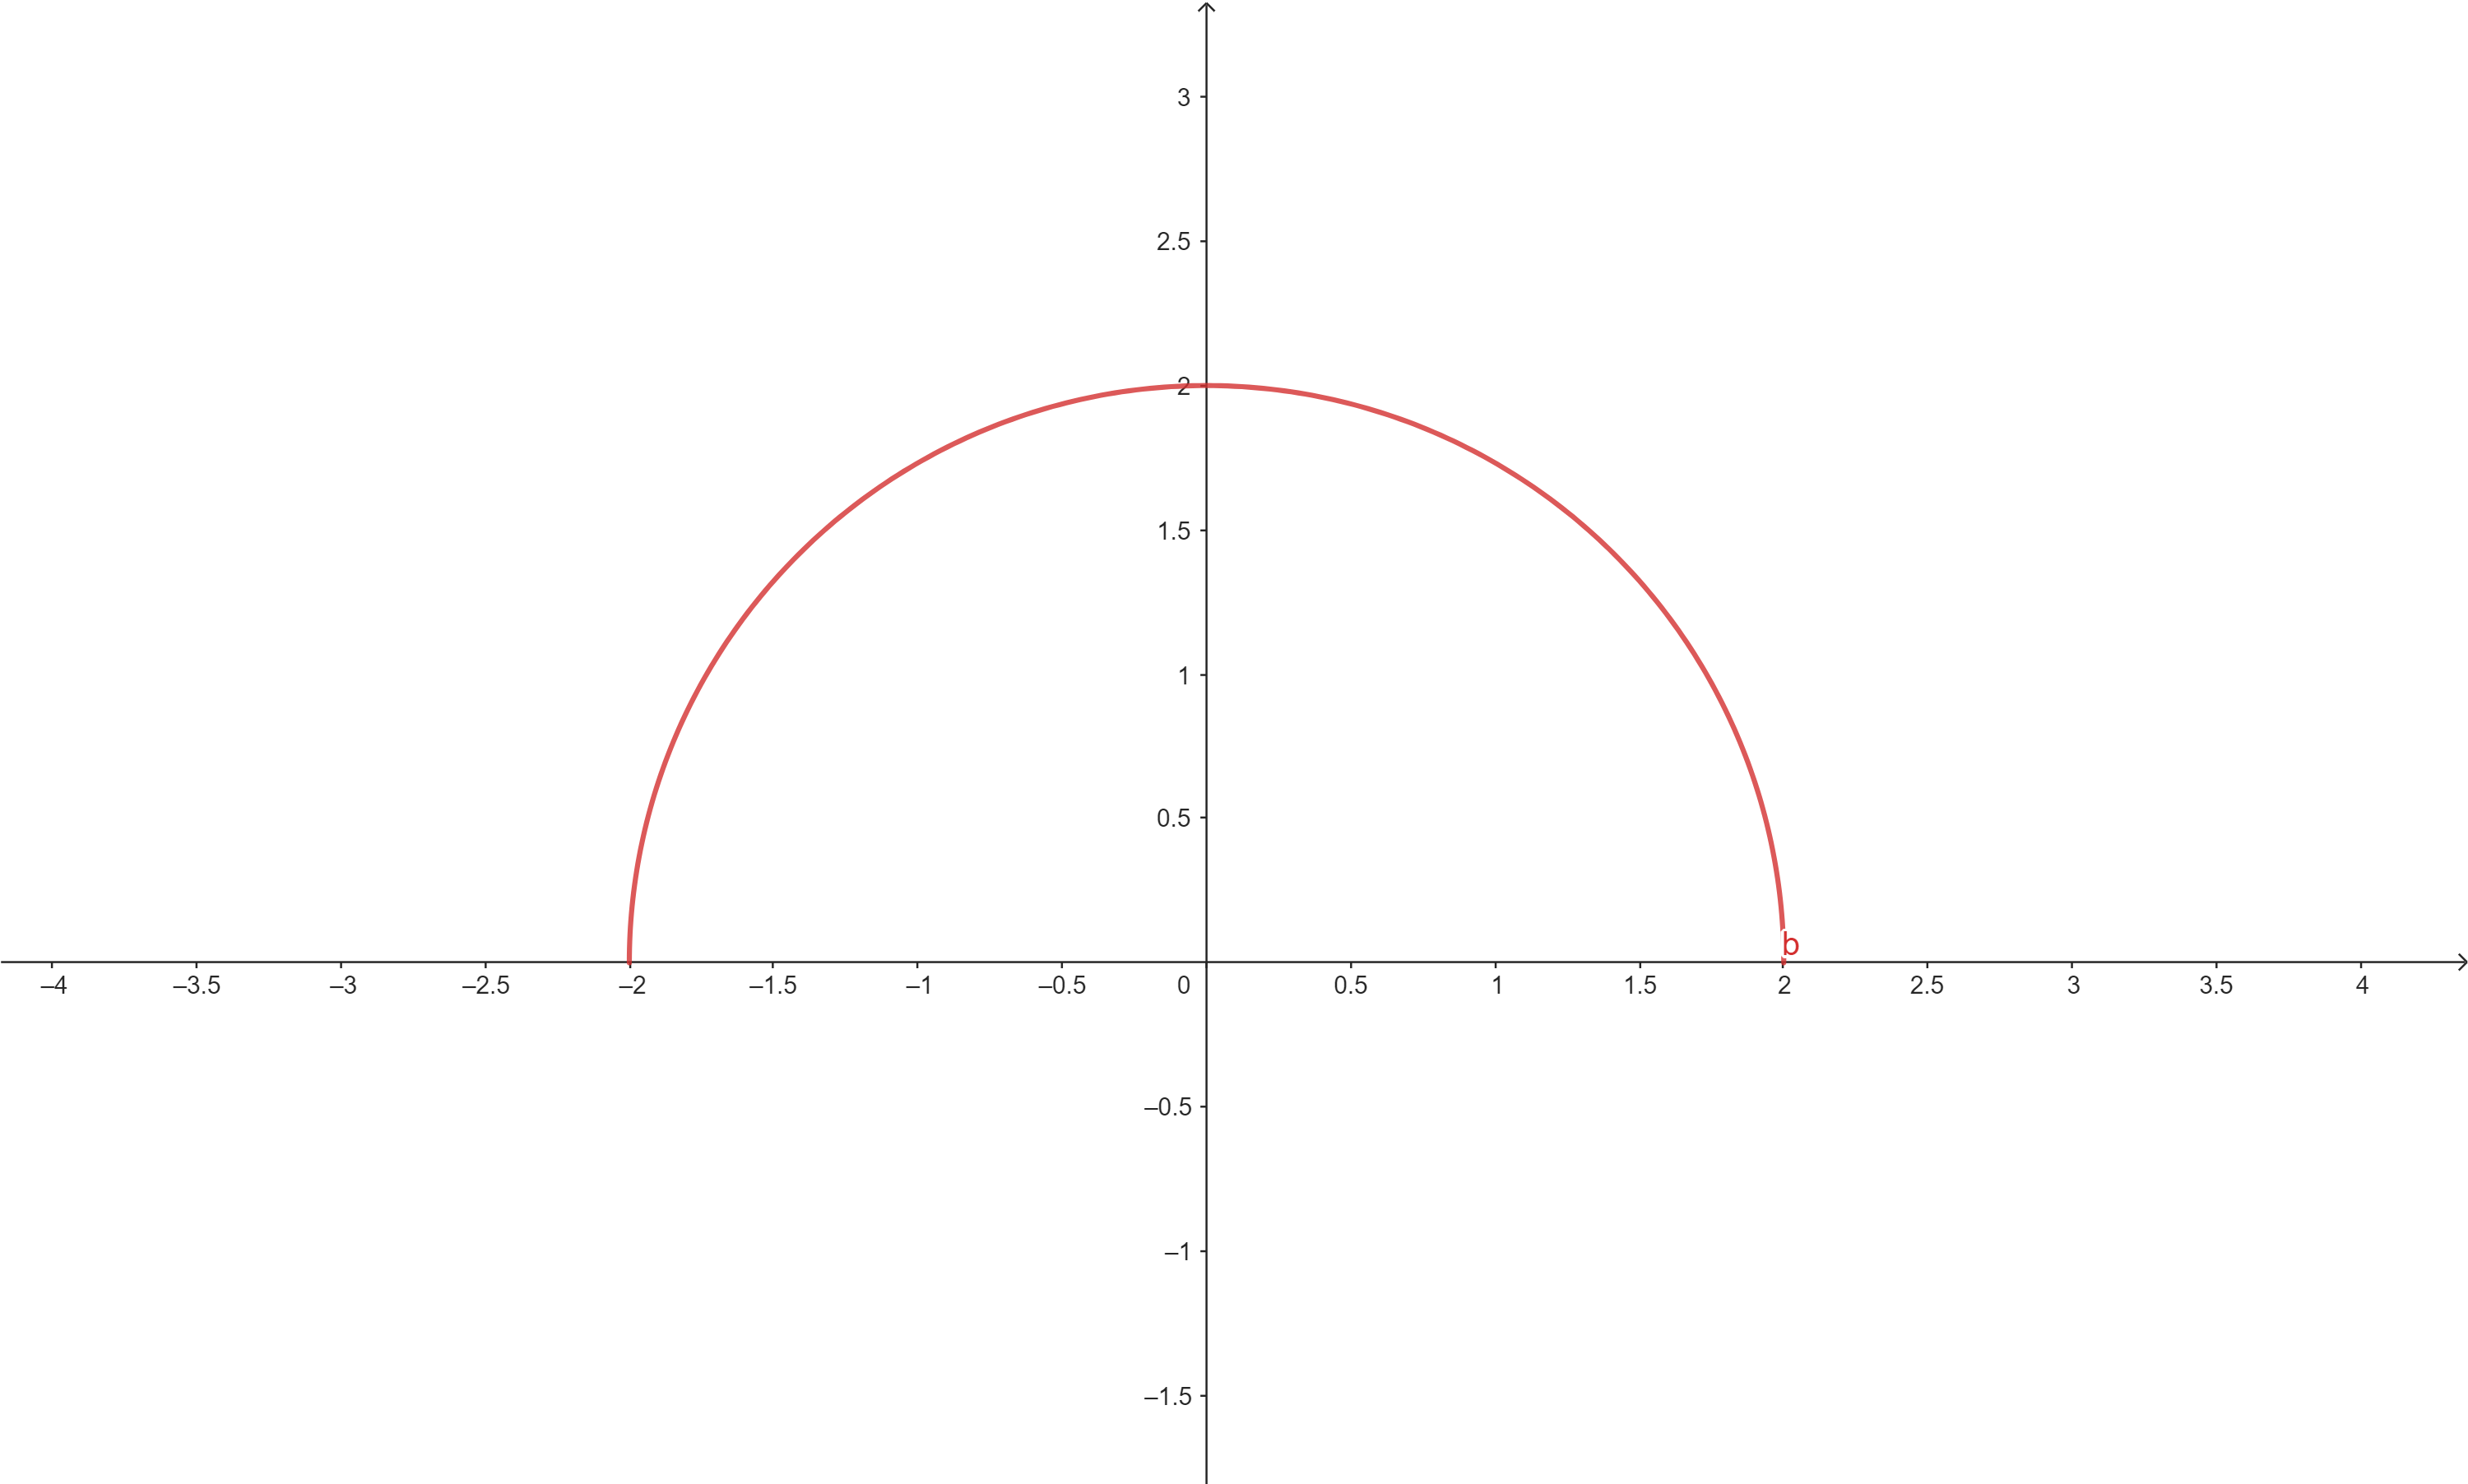
\includegraphics[width=\textwidth]{Capitoli/Capitolo1/sostegno_circ1.png}
        \caption{Sostegno di $\varphi(t)$ con $R=2$ e $t\in[0, \pi]$}
    \end{minipage}
    \hspace{1cm}
    \begin{minipage}{0.25\textwidth}
        \centering
        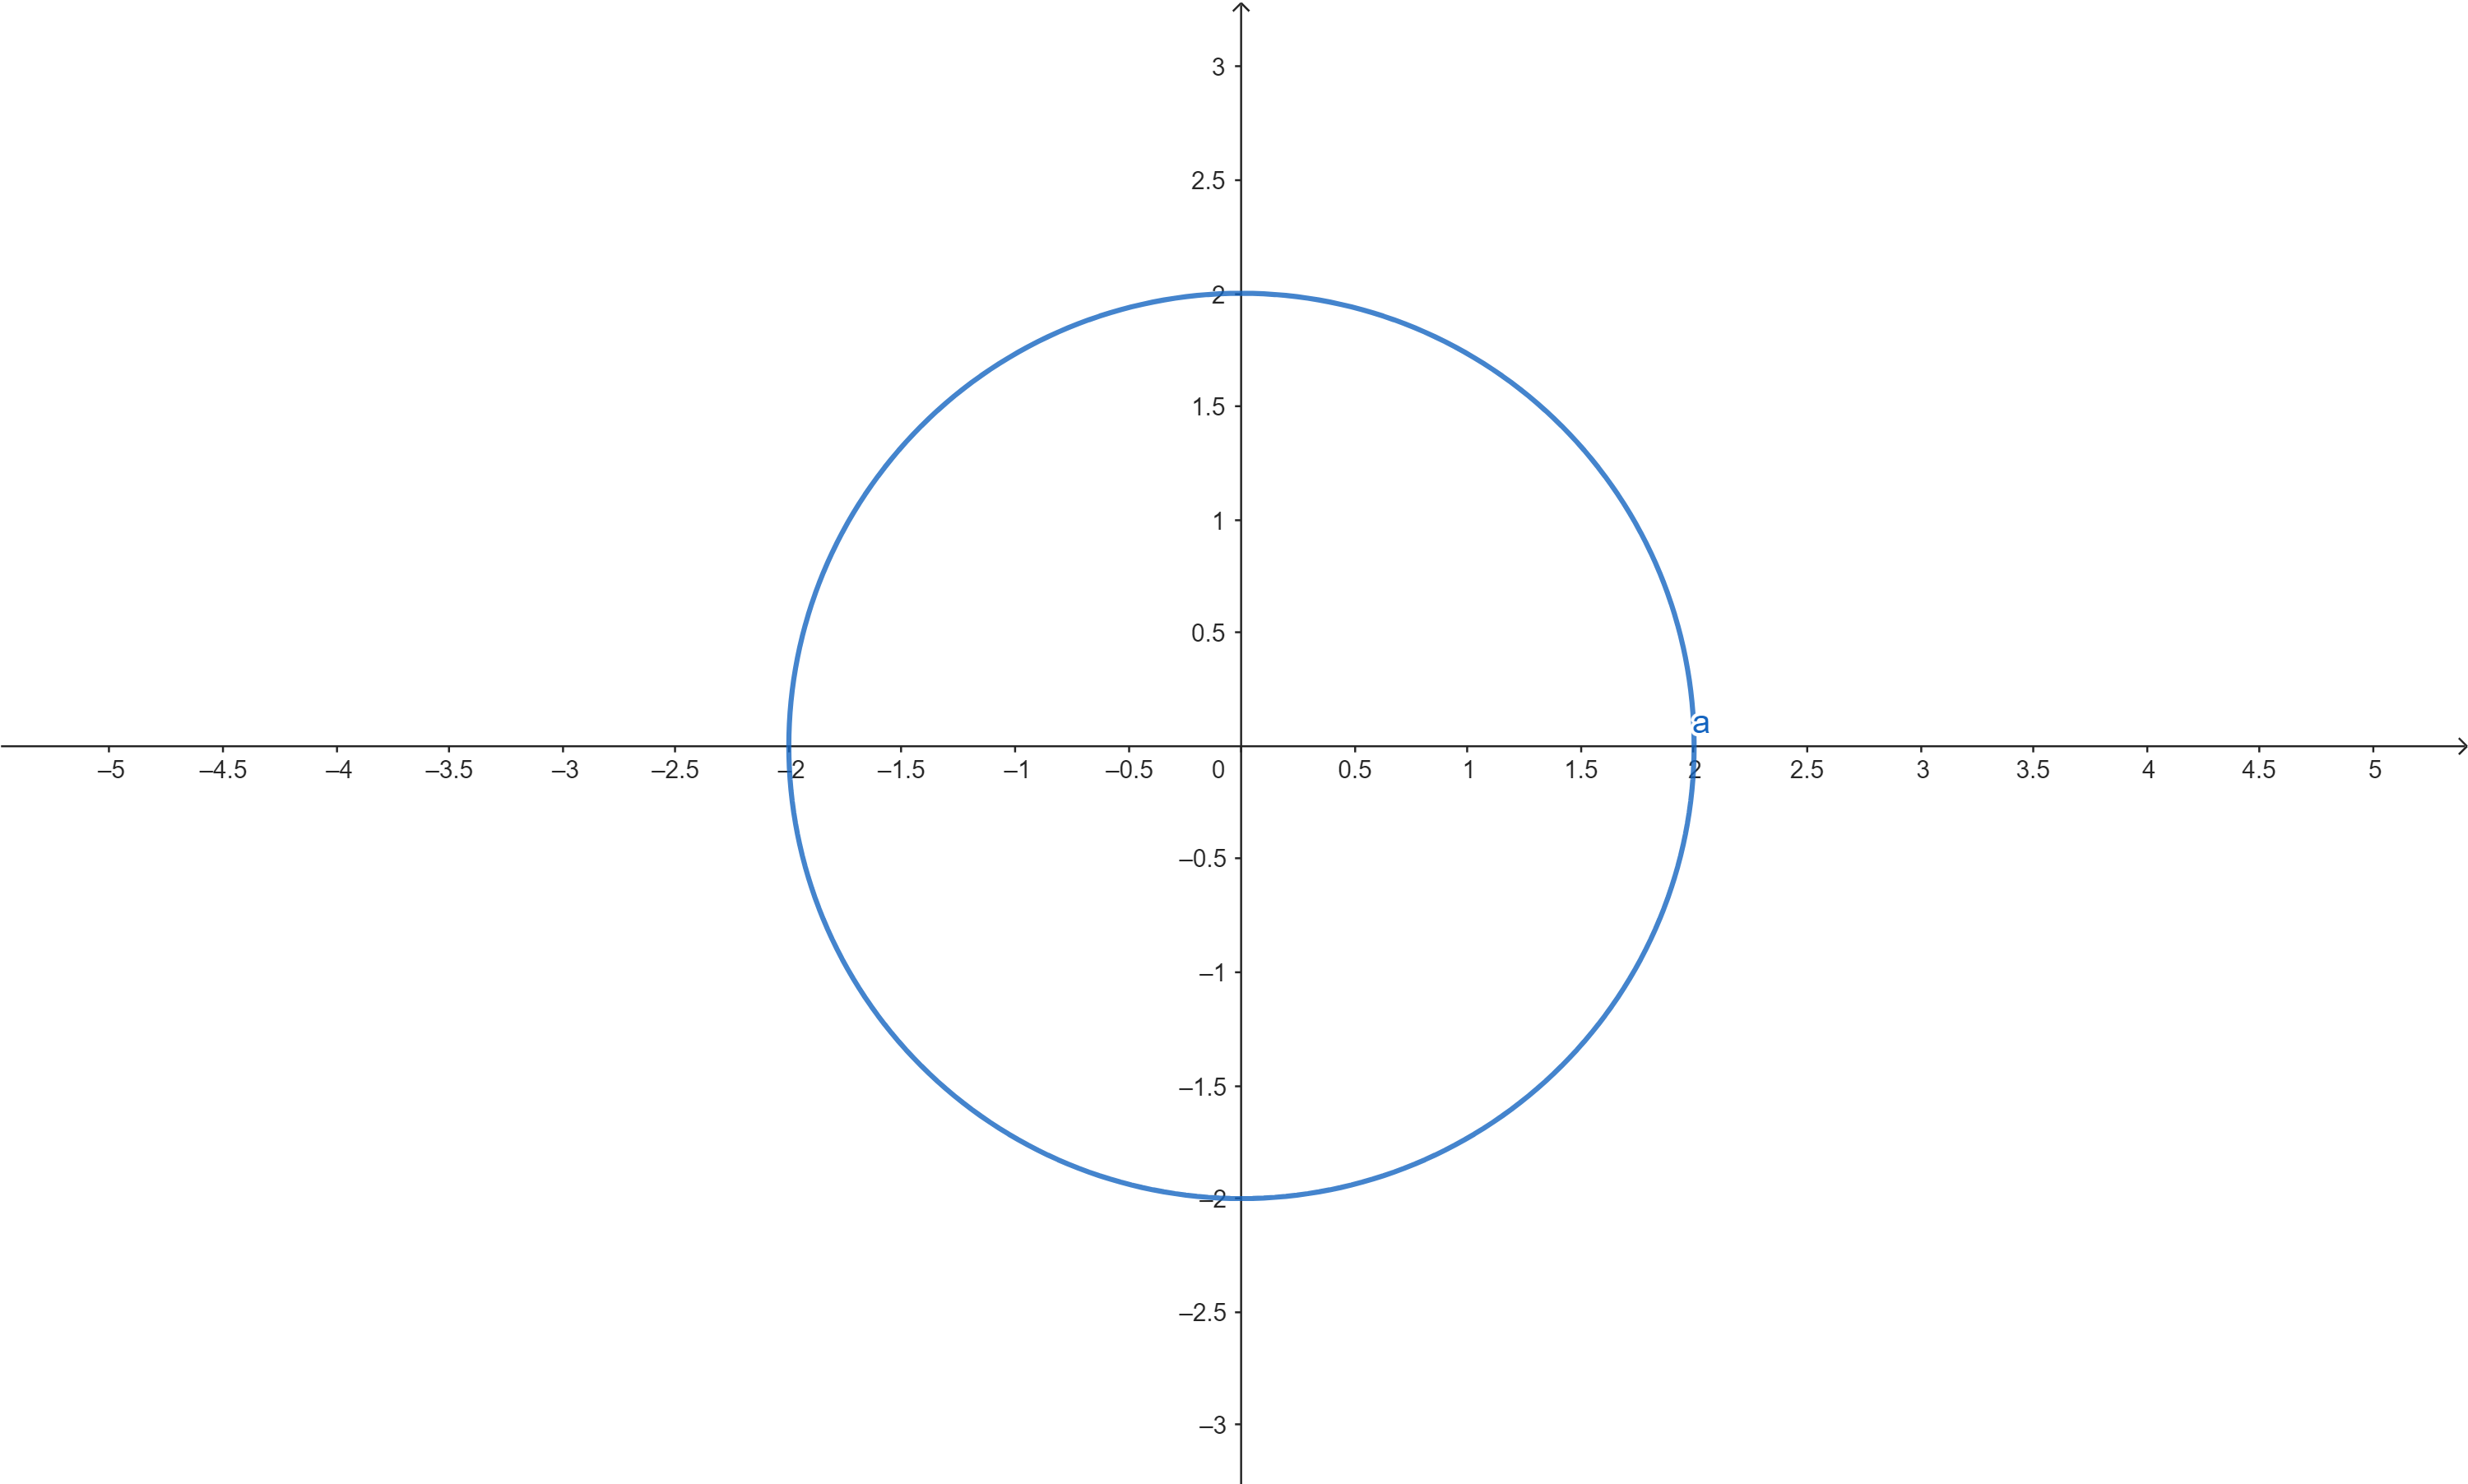
\includegraphics[width=\textwidth]{Capitoli/Capitolo1/sostegno_circ2.png}
        \caption{Sostegno di $\varphi(t)$ con $R=2$ e $t\in[0, 2\pi]$}
    \end{minipage}
    \hspace{1cm}
    \begin{minipage}{0.25\textwidth}
        \centering
        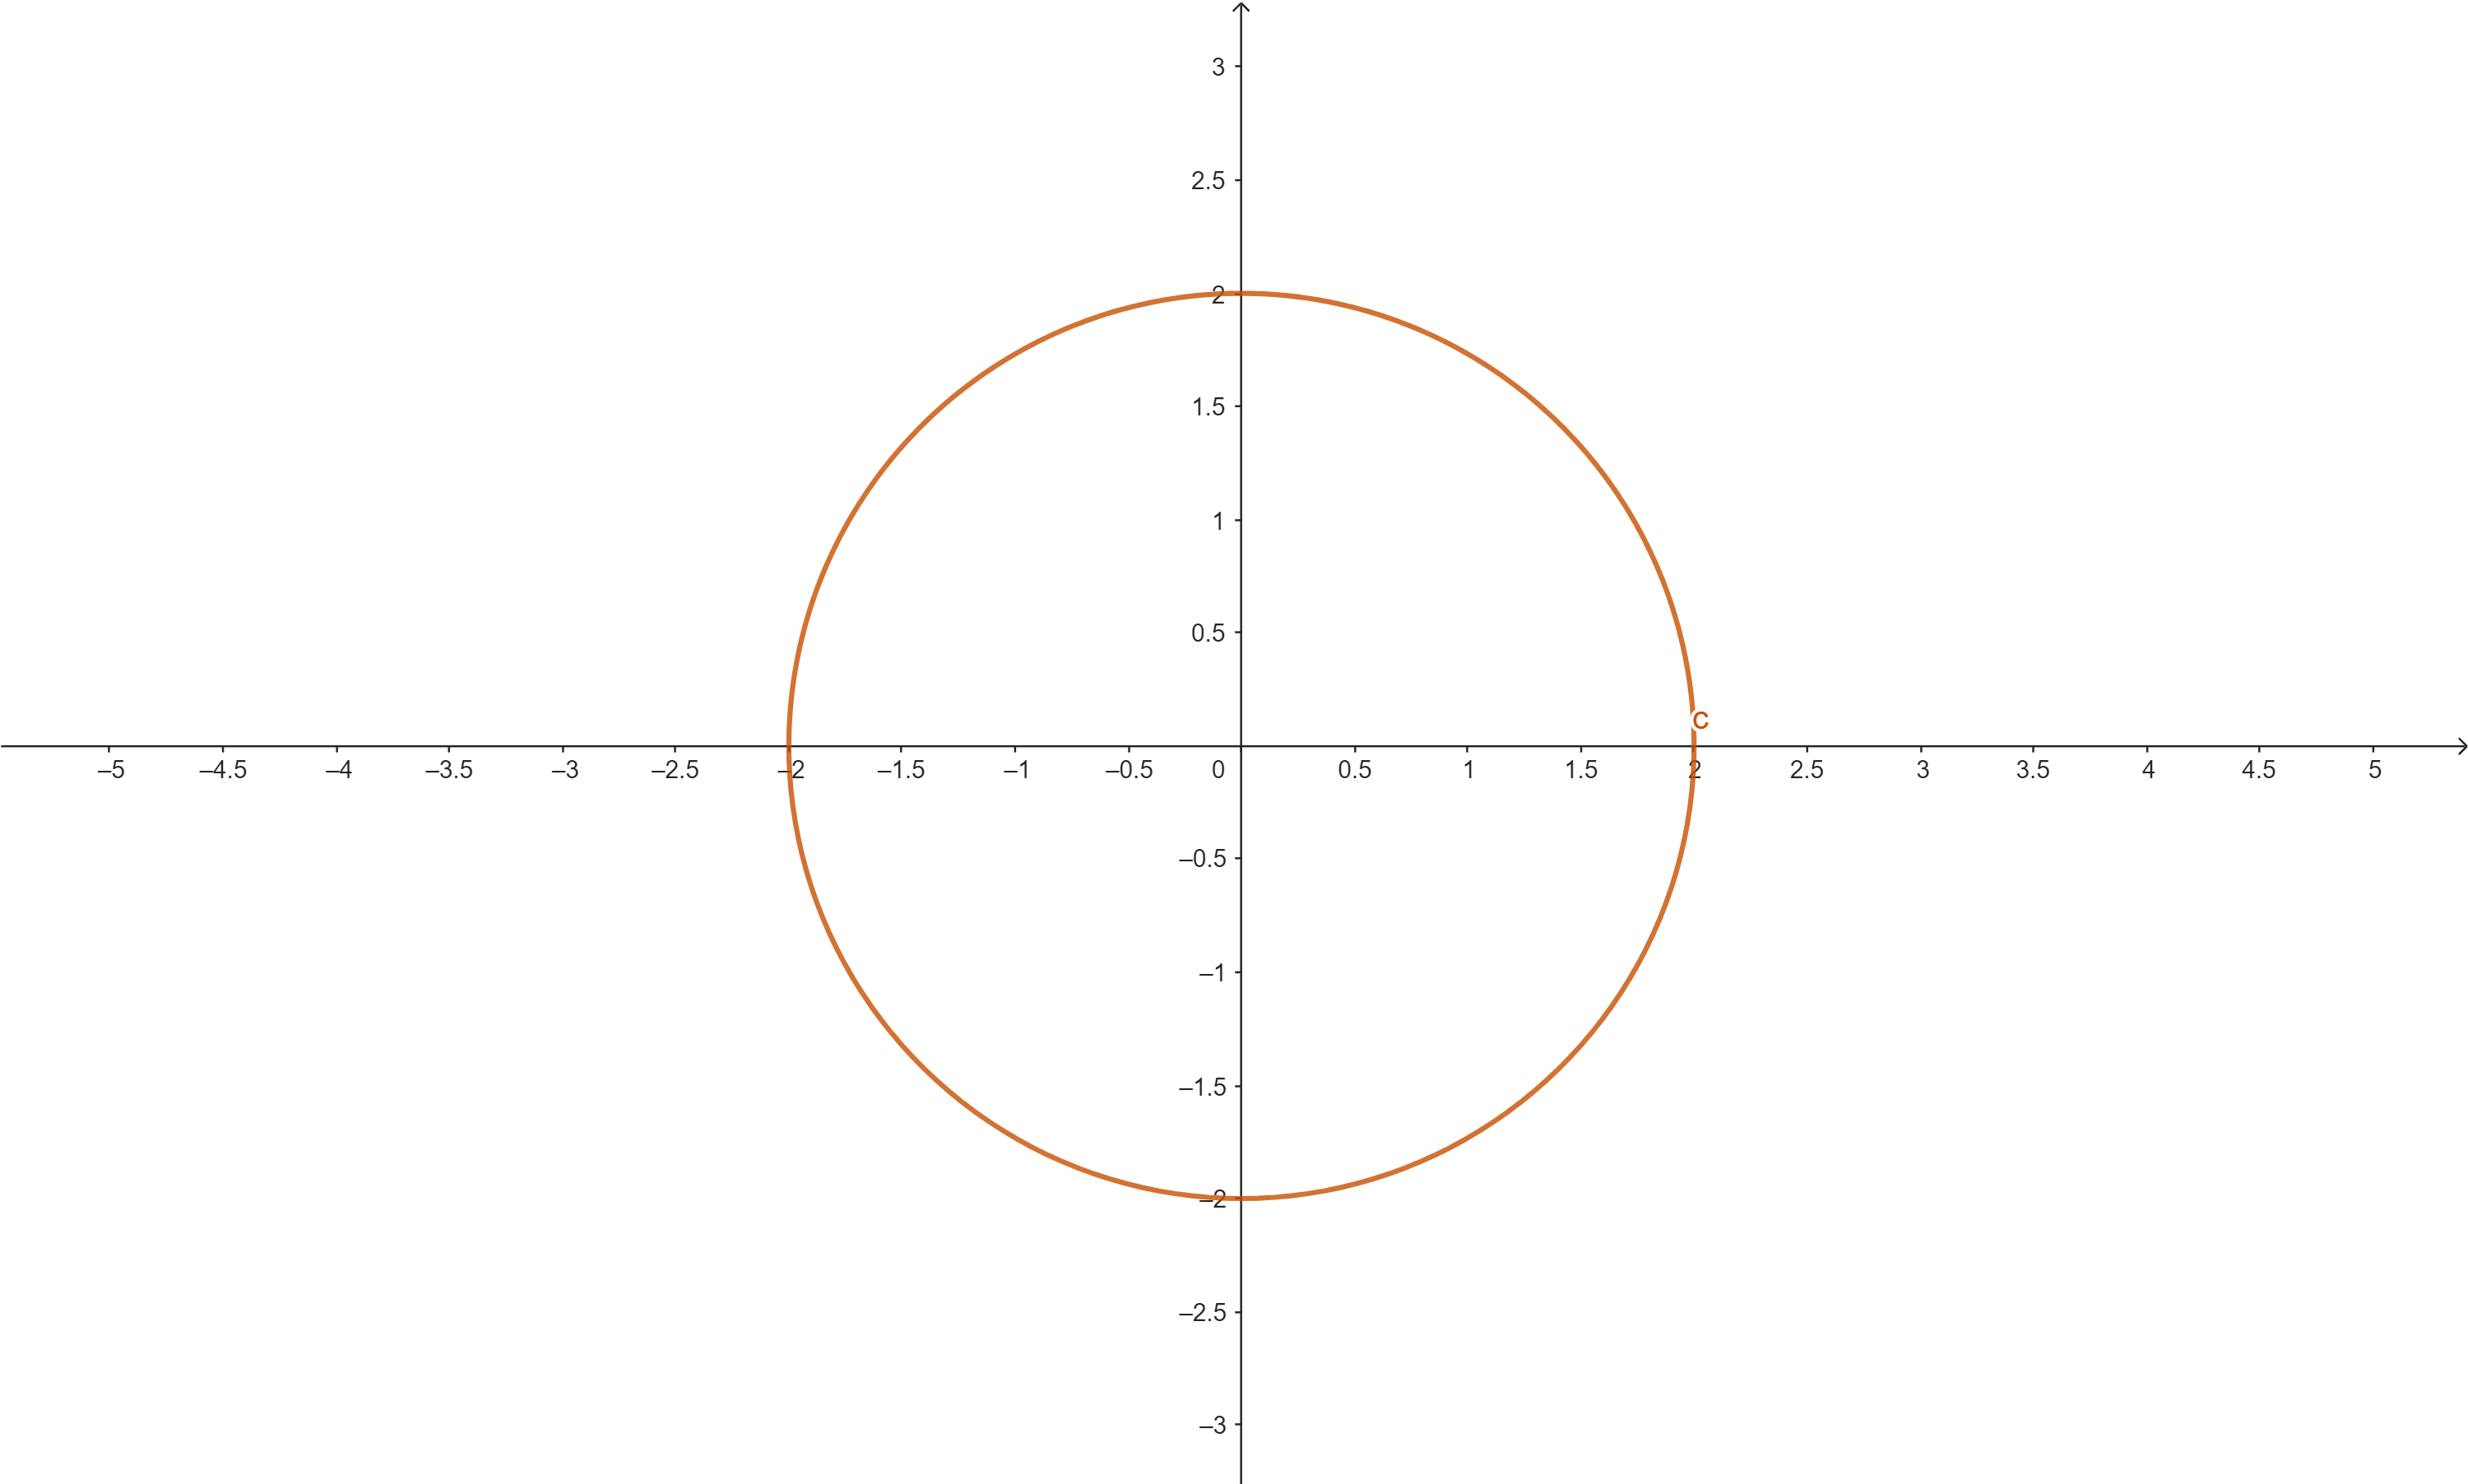
\includegraphics[width=\textwidth]{Capitoli/Capitolo1/sostegno_circ3.png}
        \caption{Sostegno di $\varphi(t)$ con $R=2$ e $t\in[0, 3\pi]$}
    \end{minipage}
\end{figure}
\end{example}
Da ciò si può osservare come, \textit{in primis}, la definizione di $I$ sia fondamentale nel tracciare il sostegno e, \textit{in secundis}, come, d'altra parte, il sostegno non identifichi la curva. A tal proposito infatti occorre notare che, benché le curve associate ai sostegni delle figure 1.2 e 1.3 siano diverse, i loro sostegni sono uguali.
\begin{example}    
    Un'altra casistica è quella rappresentata dalla curva di equazione $\varphi(t)=(R \cos(-t), R \sin(-t))$. Il suo sostegno, infatti, rimane la circonferenza (o l'arco) di raggio $R$, percorso tuttavia in senso orario.
\end{example}
\begin{definition}
    Sia $\varphi:[I \to \mathbb{R}^n]$ una curva parametrica. Allora si dice che $P_1=\varphi(t_1)$ \textbf{precede} $P_2=\varphi(t_2)$ nel verso delle $t$ crescenti se $t_1<t_2$ con $t_1, t_2 \in I$.
\end{definition}
\subsection{Proprietà delle curve parametriche}
Fatte tali premesse, si passi ad analizzare alcune proprietà delle curve.
\begin{definition}
    Una curva $\varphi:[a,b]\to\mathbb{R}^n$ si dice \textbf{chiusa} se $\varphi(a)=\varphi(b)$.
\end{definition}
\begin{oss}
    Si noti a tal proposito che la curva in figura 1.3 non è chiusa, mentre quella in figura 1.2 sì.
\end{oss}
\begin{definition}
    Una curva $\varphi:[a,b] \to \mathbb{R}^n$ si dice \textbf{semplice} se, $\forall$ $ t_1, t_2 \in [a,b]$ distinti di cui almeno uno \textit{interno} all'intervallo, risulta $\varphi(t_1)\neq\varphi(t_2)$.
\end{definition}
    \begin{oss}
        In altre parole, affinché $\varphi$ sia semplice, essa non deve autointersecarsi, se non, al più, negli estremi.
    \end{oss}
    \begin{oss}
        La curva in figura 1.2 è semplice.
    \end{oss}
\begin{definition}
    Una curva $\varphi:[a,b] \to \mathbb{R}^n$ si dice \textbf{regolare} se l'applicazione $\varphi$ è di classe $C^1$ in $[a,b]$ e se, $\forall t \in (a,b)$ il vettore $\varphi'(t)$ è diverso dal vettore nullo.
\end{definition}
A fronte di ciò, è possibile osservare che, se una curva è regolare, presi due valori distinti del parametro $t$, come $t_0, t_1$, è possibile tracciare la retta passante per $\varphi(t_0), \varphi(t_1)$. Allora, per $t_1 \to t_0$ si ottiene la \textbf{retta tangente} alla curva $\varphi$ in $\varphi(t_0)$.
Si definisce allora $\varphi'(t_0)=(\varphi_1'(t_0), \dots, \varphi_n'(t_0))$ \textbf{vettore tangente} alla curva $\varphi$ in $\varphi(t_0)$.
\begin{definition}
    Se $\varphi$ è regolare, si definisce \textbf{versore tangente} il normalizzato del vettore tangente a $\varphi$ in $\varphi(t_0)$, ovvero:
    \begin{equation}
        T(t_0)=\frac{\varphi'(t_0)}{|\varphi'(t_0)|}
    \end{equation}
\end{definition}
    \begin{oss}
        Data questa informazione, può diventare utile valutare direttamente $|\varphi'(t)|$ per stabilire la regolarità di una curva. Tale quantità è talvolta definita \textbf{velocità scalare}.
    \end{oss}
    \begin{oss}
        Una curva regolare è priva di cuspidi o punti angolosi.
    \end{oss}
\begin{example}
    Si valuti ora la seguente curva: $\varphi(t)=(t^3, t^2)$ con $t \in [-1, 1]$.
    Rispetto alle proprietà elencate, si può affermare che:
    \begin{itemize} 
        \item non è chiusa perché $\varphi(-1)=(-1,1)\neq(1,1)=\varphi(1)$;
        \item è semplice perché se fosse $\varphi(t_1) = \varphi(t_2)$, allora si avrebbe:
$
\begin{cases}
    t_1^3 = t_2^3 \\
    t_1^2 = t_2^2
\end{cases}
$
\\Ciò però significa che $t_1=t_2$.
    \item non è regolare poiché la sua derivata $\varphi(t)=(3t^2, 2t)$ si annulla in entrambe le componenti per $t=0$.
    \end{itemize}
Può essere utile visualizzare tale curva riscrivendone le equazioni in forma cartesiana. Si ricava dalla prima componente che $x=t^3 \iff t=x^\frac{1}{3}$. Allora, sostituendo nella seconda componente, $y=t^2 \iff y=\left(x^\frac{1}{3}\right)^2 \iff y=x^\frac{2}{3}$. Il grafico di tale funzione mostra, per l'appunto, la presenza di una cuspide in $t=0$, come già osservato in precedenza.\\
Tuttavia si può anche osservare che la curva può essere vista come l'unione di due curve regolari $\varphi_+$ nel semiasse positivo e $\varphi_-$ nel semiasse positivo negativo.
\end{example}
\begin{definition}
    Una curva $\varphi:[a,b]\to\mathbb{R}^n$ si dice \textbf{regolare a tratti} se esiste una suddivisione di $[a,b]$ in un numero \textit{finito} di intervalli $[t_i, t_{i+1}]$ in cui $\varphi$ sia regolare.
\end{definition}
\subsubsection{Curve cartesiane}
    Si studino ora le cosiddette curve \textbf{cartesiane}, definite come: 
    \begin{equation}
        y=f(x) \text{ con } x \in [a,b] 
    \end{equation}
    cioè, in forma parametrica,
    \begin{equation}
        \begin{cases}
            x=t \text{ con } t\in[a,b]\\ y=f(t)
        \end{cases}\\
    \end{equation}
    Di esse si può osservare che se, $f \in C^1$ allora la curva è regolare. Inoltre le curve cartesiane sono sempre semplici, giacché $t$ è iniettiva, e non sono mai chiuse.

\subsubsection{Curve in coordinate polari}
    Altre curve da analizzare sono le curve \textbf{in forma polare} ovvero del tipo:
    \begin{equation}
        \varrho=\varrho(\theta) 
    \end{equation}
    oppure in forma parametrica come 
    \begin{equation}
        \begin{cases}
            x=\varrho(\theta)\cos(\theta)\\
            y=\varrho(\theta)\sin(\theta)
        \end{cases}
    \end{equation}
    con $(x,y) \in \mathbb{R}\setminus \left\{(0,0)\right\}$, $\varrho \in \left[0, +\infty\right]$ e $\theta \in \left[0, 2\pi\right]$.\\
    Tale specifica rispetto alle caratteristiche della curva serve a sottolineare il fatto che una curva che si annulli in un qualche punto a causa di $\varrho=0$ e $\theta$ conseguentemente non definito, non sia regolare.\\
    Si noti che nel caso di una circonferenza il raggio $\varrho(t)=\text{cost}$.\\
    Il tangente in questo caso è
    \begin{equation}
        (x'(\theta), y'(\theta))=(\varrho'(\theta)\cos(\theta)-\varrho(\theta)\sin(\theta), \text{ } \varrho'(\theta)\sin(\theta)+\varrho(\theta)\cos(\theta))
    \end{equation}
    Dunque la norma della curva è:
    \begin{equation}
        |(x'(\theta), y'(\theta))|=\sqrt{\varrho'^2(\theta)+\varrho^2(\theta)}
    \end{equation} 
    Ne consegue che, se la curva non ha zeri doppi in $\left(\theta_1, \theta_2\right)$, allora è regolare in $\left[\theta_1, \theta_2\right]$.\\
    Si prenda ora il caso specifico in cui $\varphi$ è una curva in coordinate polari e $[a,b] \subseteq [0, 2\pi]$.
    Per quanto riguarda la proprietà di chiusura della curva, si presentano due scenari: 
    \begin{itemize}
        \item Se $[\theta_0, \theta_1] \subsetneq [0, 2\pi]$ allora la curva è chiusa per $\varrho(\theta_0)=\varrho(\theta_1)=0$;
        \item Se $[\theta_0, \theta_1]=[0, 2\pi]$ allora la curva è chiusa per $\varrho(0)=\varrho(2\pi)$
    \end{itemize}
    Rispetto alla proprietà di semplicità, si osserva:
    \begin{itemize}
        \item Se $[\theta_0, \theta_1] \subseteq [0, 2\pi]$ allora la curva è semplice se $\nexists$ $\theta_i, \theta_j \in (0,2\pi)$ tali che $\varrho(\theta_i)=\varrho(\theta_j)=0$
    \end{itemize}
\newpage
\section{Curve equivalenti}
\begin{definition}
    Due curve $\varphi: I\to \mathbb{R}^n$ e $\psi:J\to \mathbb{R}^n$ si dicono \textbf{equivalenti} se $\exists$ $\eta:I\to J$ di classe $C^1(I)$ suriettiva e tale che $\eta'(t) \neq 0$ $\forall$ $t \in I$ per cui si abbia
    \begin{equation}
        \varphi(t)=\psi(\eta(t)) \text{ } \forall \text{ } t \in I
    \end{equation}
\end{definition}
\begin{oss}
    $\eta$ è detta \textbf{cambio di parametro ammissibile}. 
\end{oss}
\begin{oss}
    Volendo studiare il segno delle curve, si ottiene:
    \begin{equation*}
        \varphi'(t)=\psi'(\eta(t))\eta'(t)
    \end{equation*}
    Si noti che $\eta'$ non turba la regolarità della curva poiché mantiene il proprio segno e non si annulla mai (per costruzione).
\end{oss}
\begin{oss}
    $\eta$ è per sua costruzione suriettiva e monotona, dunque è anche iniettiva. Pertanto $\eta$ è biunivoca e invertibile. Sfruttando $\eta^{-1}(s)$ si ottiene:
    \begin{equation}
        \psi(s)=\varphi(\eta^{-1}(s))
    \end{equation}
\end{oss}
\begin{oss}
    Se $\varphi$ e $\psi$ sono equivalenti come descritto, allora
    \begin{equation}
        \varphi\sim\psi
    \end{equation}
    Si tratta proprio di una relazione di equivalenza dal momento che:
    \begin{equation}
        \text{Per } \eta(t)=t \text{, } \varphi(t)=\varphi(\eta(t))=\varphi(t), \text{ cioè } \varphi\sim\varphi
    \end{equation}
    Il risultato dell'osservazione precedente mostra che se $\varphi\sim\psi$ allora $\psi\sim\varphi$.
    Infine, prese $\varphi$, $\psi$, $\chi$ tali che $\varphi\sim\psi$ e $\psi\sim\chi$ allora:
    $\varphi=\psi(\eta(t))$ e $\psi(t)=\chi(\zeta(t))$. Allora
    \begin{equation}
        \varphi(t)=\psi(\eta(t))=\chi(\zeta(\eta(t))) \text{ cioè } \varphi\sim\chi
    \end{equation}
\end{oss}
\begin{definition}
    L'applicazione $\eta$ che permette di passare dalla rappresentazione parametrica di $\varphi$ a quella di $\psi$ è detta anche \textbf{$C^1$ diffeomorfismo}.
\end{definition}
\begin{definition}
    Date due curve equivalenti $\varphi$ e $\psi$, si dice che $\psi$ è la riparametrizzazione di $\varphi$.
\end{definition}
Si può osservare che due curve equivalenti hanno lo stesso sostegno. Tuttavia tale condizione non è sufficiente siccome per l'equivalenza è necessario che il sostegno sia percorso nel medesimo numero di volte.\\
La nozione di equivalenza può essere rafforzata, come segue.
\begin{definition}
    Due curve equivalenti come sopra si dicono \textbf{equvalenti con lo stesso verso} se il loro sostegno è percorso nello stesso verso, cioè se: $\eta'>0$
\end{definition}
\section{Lunghezza di una curva}
Si consideri una curva continua $\varphi:[a,b] \to \mathbb{R}^n$ definita su un intervallo chiuso e limitato $[a,b]$. È possibile associare ad ogni \textit{partizione} 
\begin{equation}
    a=t_0<t_1<...<t_N=b
\end{equation}
la poligonale $\mathcal{P}$ inscritta nella curva e di vertici $\varphi(a),\varphi(t_1),\dots,\varphi(t_{N-1}), \varphi(b)$. La lunghezza di tale poligonale sarà pari a:
\begin{equation}
    \ell(\mathcal{P})=\sum\limits_{i=1}^{N}{|\varphi(t_i)-\varphi(t_{i-1})}
\end{equation}
Tale valore è un'approssimazione della lunghezza effettiva della curva per difetto, il cui errore diminuisce in maniera proporzionale al numero di segmenti che compongono la poligonale.
\begin{figure}[H]
    \centering
    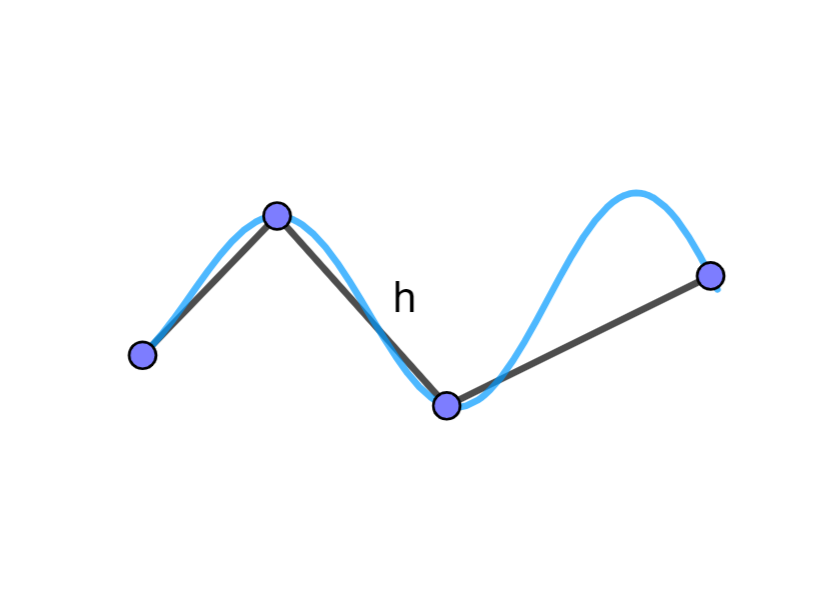
\includegraphics[width=0.33\textwidth]{Capitoli/Capitolo1/lunghezza1.png}
    \hspace{0.05\textwidth} % Spazio tra le immagini
    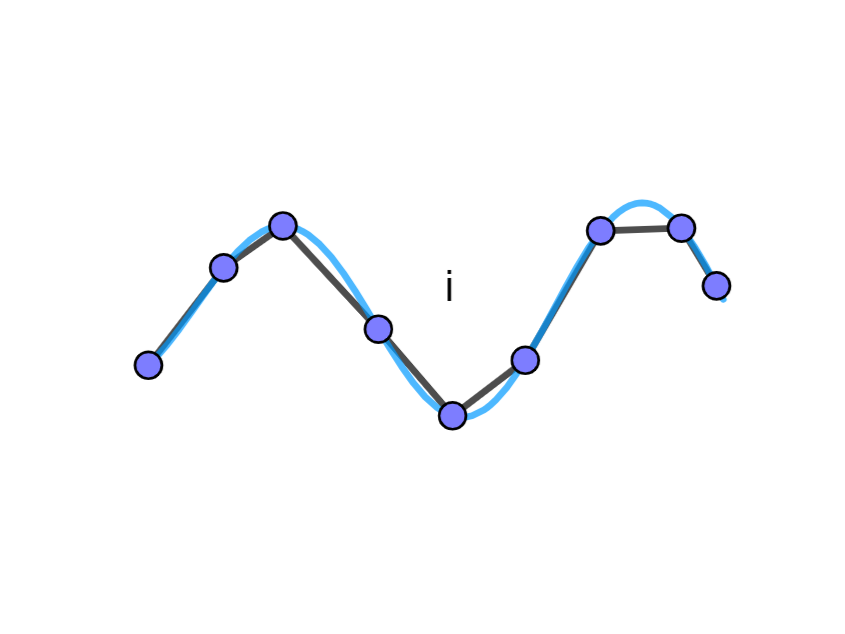
\includegraphics[width=0.33\textwidth]{Capitoli/Capitolo1/lunghezza2.png}
    \caption{In figura la stessa curva la cui lunghezza viene misurata con poligonali diverse.}
\end{figure}
\begin{definition}
    Sia $\varphi:[a,b]\to \mathbb{R}^n$, allora si dice \textbf{lunghezza di un arco di curva} continua la quantità
    \begin{equation}
        L(\varphi)=\sup\limits_{l}(\mathcal{P})
    \end{equation}
    dove $\mathcal{P} \in \Pi$ con $\Pi=\left\{\text{poligonali inscritte nella curva}\right\}$.
\end{definition}
\begin{definition}
    Si dice che una curva $\varphi: [a,b] \to \mathbb{R}^n$ è \textbf{rettificabile} se 
    \begin{equation}
        \sup\limits_{\mathcal{P}\in\Pi}L(\varphi)<+\infty
    \end{equation}
\end{definition}
\begin{theorem}[Teorema di rettificabilità]
Sia $\varphi: [a,b] \to \mathbb{R}^n$ una curva di classe $C^1$. Allora essa è rettificabile e 
\begin{equation}
    L(\varphi)=\int_{a}^{b}{|\varphi'(t)|dt}
\end{equation}
\end{theorem}
\begin{oss}
    La lunghezza di una curva $C^1$ è invariante per riparametrizzazione.
\end{oss}
\begin{oss}
    Si osservi che vale: $\ell(\mathcal{P})\leq \int_{a}^{b}{|\varphi'(t)|dt}$. Infatti:
    \begin{equation}
        \begin{aligned}
            \ell(\mathcal{P}) &= \sum\limits_{i=1}^{N} \left| \varphi(t_i) - \varphi(t_{i-1}) \right|= \sum\limits_{i=1}^{N} \left\lvert \int_{t_{i-1}}^{t_i} \varphi'(t) \, dt \right\rvert \\
            &\leq \sum\limits_{i=1}^{N} \int_{t_{i-1}}^{t_i} \left\lvert \varphi'(t) \right\rvert \, dt = \int_{a}^{b} \left\lvert \varphi'(t) \right\rvert \, dt
        \end{aligned}
    \end{equation}
\end{oss}
\begin{example}
    Detta 
    \begin{equation*}
        f(x)= \begin{cases}
            0 \text{ se } x=0\\ x\sin(\frac{1}{x}) \text{ se } x\neq 0
        \end{cases}
    \end{equation*}
    allora una curva non rettificabile può essere 
    \begin{equation*}
        \varphi(t)=(t, f(t)) \text{ con } t\in[0,1]
    \end{equation*}
\end{example}
\section{Triedro di Frénet}
Si desideri ora sviluppare un sistema di riferimento intrinseco ad una curva $\varphi:[a, b] \to \mathbb{R}^n$ regolare e tale che $\varphi'(t)$ ed il versore tangente $T$ siano ben definiti su $(a, b)$.
\begin{definition}
    Si definisce l'\textbf{ascissa curvilinea} o parametro d'arco $s=s(t)$ come
    \begin{equation}
        s(t)=\int_a^t{\left\lvert \varphi'(\tau) \right\rvert d\tau}
    \end{equation}
    \end{definition}
    \begin{oss}
        $s:[a,b] \to [0, L(\varphi)=L]$ è una parametrizzazione della curva regolare $\varphi$. Inoltre, $s'(t)=|\varphi'(t)| \neq 0$ su $(a,b)$.
    \end{oss} 
    \begin{oss}
        Riparametrizzando $\varphi$ con ascissa curvilinea $s=s(t)$, si può dire che $\varphi\sim\psi$. Dunque, rinominata $t(s)=s^{-1}(t)$, vale $\psi(s)=\varphi(t(s))$. Derivando la riparametrizzazione, si ha che:
        \begin{equation}
            \psi'(s)=\varphi'(t(s)) \text{ } t'(s) \overset{\substack{\text{Derivata}\\\text{ inversa}}}{=} \frac{\varphi'(t(s))}{s'(t)} = \frac{\varphi'(t(s))}{|\varphi'(t(s))|}
        \end{equation}
        Ciò mostra come il vettore tangente a $\psi$ sia in ogni punto un versore tangente $T(s)$
    \end{oss}

\paragraph*{Prodotto scalare in $\mathbb{R}^n$}
Siano $\underline{v}=(v_1, \dots, v_n)$ e $\underline{w}=(w_1, \dots, w_n)$ vettori di $\mathbb{R}^n$. Allora
\begin{equation}
    \langle \underline{v}, \underline{w} \rangle = \sum\limits_{i=1}^{n}{v_iw_i} 
\end{equation}
\paragraph*{Prodotto vettoriale in $\mathbb{R}^3$}
Siano $\underline{v}=(v_1, v_2, v_3)$ e $\underline{w}=(w_1, w_2, w_3)$ vettori di $\mathbb{R}^3$. Allora
\begin{equation}
    \underline{v} \wedge \underline{w}=
    \left\lvert\begin{matrix}
         e_1 & e_2 & e_3 \\
               v_1 & v_2 & v_3 \\
               w_1 & w_2 & w_3
            \end{matrix}\right\rvert
\end{equation}
\begin{lemma}
    Siano $u, v$ definiti in $I\to\mathbb{R}^3$ e derivabili. Allora:
    \begin{align}
        \frac{d}{dt}{\langle u(t), v(t) \rangle} = \langle u'(t), v(t) \rangle + \langle u(t), v'(t) \rangle \\
        \frac{d}{dt}\left(u(t) \wedge v(t)\right) = u'(t) \wedge v(t) + u(t) \wedge v'(t)
    \end{align}
\end{lemma}
\begin{proposition}
    Sia $w:I\to\mathbb{R}^3$ derivabile e tale che $\exists$ $c>0$ per cui $|w(t)|=c$ $\forall$ $t \in I$. Allora $w'(t) \perp w(t)$.
\end{proposition}
    \begin{proof}
        Affinché i due vettori siano ortogonali, occorre che il loro prodotto scalare sia nullo. Pertanto, poiché per ipotesi $|w(t)|=c$
        \begin{equation}
            |w(t)|^2=c^2 \iff \langle w(t), w(t) \rangle = c
        \end{equation}
        Derivando rispetto a $t$ e applicando l'equazione 1.26, si ha che:
        \begin{equation}
            \frac{d}{dt}{\langle w(t), w(t)\rangle}\overset{\substack{\text{Prop.} \\ \text{prod. scal.} }}{=}2 \langle w'(t), w(t) \rangle = \frac{d c^2}{dt}=0
        \end{equation}
    \end{proof}
\begin{oss}
    La curva $\psi:[c,d] \to \mathbb{R}^3$ parametrizzata con ascissa curvilinea è tale che $|\psi'(s)|=1$. Di conseguenza, per la proposizione, $\psi''(s) \perp \psi'(s)$ e, nella fattispecie, $T'(s) \perp T (s)$.  
\end{oss}
\begin{definition}
    Sia $\psi$ una riparametrizzazione di $\varphi$ biregolare nel suo intervallo di parametrizzazione, cioè sia tale che $\psi \in C^2([c,d])$ e $\psi''(s) \neq 0$ $\forall$ $s \in [c,d]$. Allora si può definire il \textbf{versore normale} il normalizzato della derivata del versore tangente. Quindi:
    \begin{equation}
        N(s)=\frac{\psi''(s)}{|\psi''(s)|}=\frac{T'(s)}{|T'(s)|}
    \end{equation}
\end{definition}
\begin{definition}
    Si dice \textbf{curvatura} di $\psi$ in $\psi(s)$ 
    \begin{equation}
        k(s)= |\psi''(s)|
    \end{equation}
\end{definition}
\begin{definition}
    Si dice \textbf{piano osculatore} per $\psi$ in $\psi(s)$ il piano generato da 
    \begin{equation}
        \left\{T(s), N(s)\right\}
    \end{equation} 
\end{definition}
È appena stato definito un nuovo versore $N$ linearmente indipendente. È possibile ottenere una base ortonormale di $\mathbb{R}^3$ attraverso il prodotto esterno dei due versori.
\begin{definition}
    Si dice \textbf{versore binormale} il versore:
    \begin{equation}
        B(s)=T(s) \wedge N(s)
    \end{equation}
\end{definition}
\begin{definition}
    Si dice \textbf{piano normale} per $\psi$ in $\psi(s)$ il piano generato da
    \begin{equation}
        \left\{N(s), B(s)\right\}
    \end{equation}
\end{definition}
\newpage
\begin{definition}
    Si dice \textbf{piano rettificato} per $\psi$ in $\psi(s)$ il piano generato da
    \begin{equation}
        \left\{ B(s), T(s) \right\}
    \end{equation}
\end{definition}
\begin{definition}
    Si dice \textbf{triedro di Frénet} o \textbf{terna intrinseca} la base ortonormale di $\mathbb{R}^3$ positivamente orientata formata da
    \begin{equation}
        \left\{T(s), N(s), B(s)\right\}
    \end{equation}
\end{definition}
\begin{theorem}[Formule di Frénet]
    Sia $\varphi: I \to \mathbb{R}^3$ una curva biregolare, di classe $C^3(I)$ e parametrizzata con ascissa curvilinea. Allora, $\exists!$ $k:I\to \mathbb{R}_+$, $\tau:I\to\mathbb{R}$ tali che:
    \begin{equation}
        \begin{cases}
            T'(s)=k(s)N(s)\\
            N'(s)=-k(s)T(s)-\tau(s)B(s)\\
            B'(s)=\tau(s)N(s)
        \end{cases}
    \end{equation}
    \end{theorem}
    \begin{proof}
        Si parta dalla prima equazione: 
        \begin{equation}
            T'(s)=k(s)N(s).        
        \end{equation}
        Tale risultato discende dalla definizione stessa di $T'$. Si consideri infatti che $T'(s)\perp T(s)$ poiché $|T(s)|=1$ $\forall$ $s$. Prendendo poi $k(s)=|T'(s)|$, si ottiene l'identità tra i due membri.\\
        Si analizzi poi la terza equazione:
        \begin{equation}
            B'(s)=\tau(s)N(s)
        \end{equation}
        Per definizione di $B$, esso discende dal prodotto vettoriale degli altri due versori. Se ne studi la derivata:
        \begin{equation}
            B'(s)=T'(s)\wedge N(s) + T(s) \wedge N(s) \overset{\substack{T'(s)\parallel N(s)}}{=} T(s)\wedge N'(s)
        \end{equation}
        Quindi, poiché $B'(s)\perp T(s)$ e $B'(s) \perp B(s)$, allora $B'(s) \parallel N(s)$. Definendo $\tau(s)=|B'(s)|$, l'equazione è soddisfatta.\\
        Infine, si affronti la seconda equazione:
        \begin{equation}
            N'(s)= -k(s)T(s)- \tau(s)B(s)
        \end{equation}
        Siccome $\left\{T(s), N(s), B(s)\right\}$ è positivamente orientata,
        \begin{equation}
            N(s)=B(s) \wedge T(s)
        \end{equation}
        Derivando $N$, si ha che
        \begin{equation}
            \begin{aligned}
                N'(s)&=B'(s)\wedge T(s) + B(s) \wedge T'(s)=\\
                &\overset{\substack{\text{Frénet}}}{=} \tau(s)N(s)\wedge T(s) + B(s) \wedge k(s)N(s)\\
                &\overset{\substack{N \wedge T = -B\\B \wedge N =-T}}{=} -\tau(s)B(s)- k(s)T(s)
            \end{aligned}
        \end{equation}
    \end{proof}
\begin{oss}
    Risolvendo il sistema di equazioni differenziali, si potrebbe mostrare come valga anche l'implicazione inversa.
\end{oss}
\begin{oss}
    Poiché $B(s)$ è ortogonale al piano osculatore, si può notare che se esso ha derivata nulla, il piano rimane costante.
\end{oss}
\begin{definition}
    Si dice \textbf{torsione} di $\varphi$ in $\varphi(s)$
    \begin{equation}
        \tau(s)=|B'(s)|
    \end{equation}
\end{definition}
\begin{definition}
    Una curva si dice \textbf{piana} se la sua torsione è nulla, cioè se essa giace su un piano.
\end{definition}
\begin{definition}
    Si dice \textbf{cerchio osculatore} per una curva $\varphi:[a,b]\to \mathbb{R}^3$ biregolare, il cerchio giacente nel piano osculatore, avente raggio $r=\frac{1}{k(t)}$ con $k(t)$ curvatura di $\varphi(t)$ e centro sul semiasse normale a $\varphi(t)$.
\end{definition}
\begin{definition}
    Il raggio del cerchio osculatore è detto \textbf{raggio osculatore}.
\end{definition}
Nel corso dell'ultimo capitolo si è cercato di trovare una parametrizzazione di una curva in $\mathbb{R}^3$ ed è stata proposta l'ascissa curvilinea, il cui calcolo non è però sempre comodo.\\
Pertanto è possibile osservare che se una generica $\psi:[a,b]\to \mathbb{R}^3$ è una curva riparametrizzata con parametro qualunque, allora valgono su di essa le formule di Frénet generalizzate.
\begin{theorem}[Formule di Frénet generalizzate]
    Sia $\psi$ una curva riparametrizzata con parametro qualunque su cui valgano le ipotesi del Teorema 2. Allora vale:
    \begin{equation}
        \begin{cases}
            T'(t)=|\psi'(t)| k(t) N(t)\\
            N'(t)=-|\psi'(t)| k(t) T(t) - |\psi'(t)| \tau(t)B(t)\\
            B'(t)=|\psi'(t)|\tau(t)N(t)
        \end{cases}
    \end{equation}
    Dove:
    \begin{align}
        &T(t)=\frac{\psi'(t)}{|\psi'(t)|} \label{Eq: Frenet Tangente}\\
        &N(t)=\frac{T'(t)}{|T'(t)|} \label{Eq: Frenet Normale}\\
        &B(t)=\frac{\psi'(t)\wedge \psi''(t)} {|\psi'(t)\wedge \psi''(t)|} \label{Eq: Frenet Binormale}\\
        &k(t)=\frac{|\psi'(t)\wedge\psi''(t)|}{|\psi'(t)|^3} \label{Eq: Frenet Curvatura}\\
        &\tau(t)=\frac{\langle\psi'(t)\wedge \psi''(t), \psi'''(t)\rangle}{|\psi'(t)\wedge \psi''(t)|^2} \label{Eq: Frenet Torsione}
    \end{align}    
\end{theorem}
\section{Integrale curvilineo}
\begin{definition}
    Sia $\gamma$ una curva regolare e $\varphi:[a,b]\to \mathbb{R}^n$ una sua rappresentazione parametrica. Sia poi $f:A\subseteq \mathbb{R}^n \to \mathbb{R}$ una funzione in più variabili tale che $\varphi([a,b])\subseteq A$ e $f \circ\varphi$ sia continua su $[a,b]$.\\
    Allora si può definire l'\textbf{integrale curvilineo di prima specie} di f su $\gamma$
    \begin{equation}
        \int_\gamma{fds} := \int_{a}^{b}{f(\varphi(t))|\varphi'(t)|dt}
    \end{equation}
\end{definition}
\begin{theorem}[Invarianza per equivalenza di curve]
    L'integrale curvilineo di prima specie è invariante per equivalenza di curve.
\end{theorem}
    \begin{proof}
        Si ricordino innanzitutto le ipotesi:\\
        \indent $\varphi:[a,b]\to \mathbb{R}^n$ regolare, parametrizzazione di $\gamma$.\\
        \indent $f:A\subseteq\mathbb{R}^n \to \mathbb{R}$ con $\varphi([a,b]) \subseteq A$\\
        \indent $\psi:[c, d]\to \mathbb{R}^n$ regolare, parametrizzazione di $\hat{\gamma}$ e $\varphi \sim \psi$.\\
        La tesi da mostrare è:
        \begin{equation}
            \int_\gamma{f ds}=\int_{\hat{\gamma}}{f ds}
        \end{equation}
        Per definizione dell'integrale curvilineo di prima specie si ha:
        \begin{equation}
            \int_\gamma{fds}= \int_{a}^{b}{f(\varphi(t))|\varphi'(t)|dt}
        \end{equation}
        Ponendo, $s=\eta(t)$ si ha che
        \begin{equation}
            \varphi(t)=\psi(\eta(t)) \iff \varphi(\eta^{-1}(s))=\psi(s)    
        \end{equation}
        e
        \begin{equation}
            \psi'(s)=\varphi'(\eta^{-1}(s))(\eta^{-1})'(s)
        \end{equation}
        Perciò, risolvendo l'integrale con la seguente sostituzione 
        \begin{equation}
            \begin{aligned}
            &s=\eta(t) \\ &t=\eta^{-1}(s) \\ &dt=(\eta^{-1})'(s)ds
            \end{aligned}
        \end{equation}
        si ha che
        \begin{equation}
            \begin{aligned}
                &\int_\gamma{fds} = \int_{a}^{b}{f(\varphi(t))\ |\varphi'(t)|\ dt}\\
                &\overset{\text{sub}}{=} \int_{\eta(a)}^{\eta(b)}{f(\varphi(\eta^{-1}(s)))\ |\varphi(\eta^{-1}(s))|\ (\eta^{-1})'(s)\ ds}
            \end{aligned}
        \end{equation}
        Ora, dipendentemente dalla monotonia di $\eta$ si avrà:\\
        \indent$\eta^{-1}>0 \Rightarrow \ \eta(a)=c,\  \eta(b)=d,\  (\eta^{-1})'(s)>0$
        \begin{equation}
            \begin{aligned}
                &\int_{\eta(a)}^{\eta(b)}{f(\varphi(\eta^{-1}(s)))\ |\varphi'(\eta^{-1}(s))| \ (\eta^{-1})'(s)\ ds}=\\
                &\int_{c}^{d}{f(\psi(s))\ |\psi'(s)| \ ds}= \int_{\hat{\gamma}}{f \ ds}
            \end{aligned}
        \end{equation}
        \indent$\eta^{-1}<0 \Rightarrow \eta(a)=d, \ \eta(b)=c, \ (\eta^{-1})'(s)<0$
        \begin{equation}
            \begin{aligned}
                &\int_{\eta(a)}^{\eta(b)}{f(\varphi(\eta^{-1}(s)))\ |\varphi'(\eta^{-1}(s))| \ (\eta^{-1})'(s)\ ds}=\\
                &\int_{d}^{c}{f(\psi(s))\ (-|\psi'(s)|)\ ds} = \int_{c}^{d}{f(\psi(s))\ |\psi'(s)|\ ds}= \int_{\hat{\gamma}}{f\ ds}
            \end{aligned}
        \end{equation}
    \end{proof}
    \begin{oss}
        La distinzione finale discende dal fatto che, presa l'equazione 1.55 e applicatovi il modulo, se $\eta$ è crescente, si ha
        \begin{equation}
            \begin{aligned}
                |\psi'(s)|&=|\varphi'(\eta^{-1}(s))(\eta^{-1})'(s)|\overset{\substack{\text{Prop.}\\\text{Norma}}}{=}|(\eta^{-1})(s)|\ |\varphi'(\eta^{-1}(s))=\\
                &\overset{\eta'>0}{=} (\eta^{-1})'(s)\ |\varphi'(\eta^{-1})(s)|
            \end{aligned}
        \end{equation}
        se $\eta$ è decrescente,
        \begin{equation}
            \begin{aligned}
                |\psi'(s)|&=|\varphi'(\eta^{-1}(s))(\eta^{-1})'(s)|\overset{\substack{\text{Prop.}\\\text{Norma}}}{=}|(\eta^{-1})(s)|\ |\varphi'(\eta^{-1}(s))=\\
                &\overset{\eta'<0}{=} -(\eta^{-1})'(s)\ |\varphi'(\eta^{-1})(s)|
            \end{aligned}
        \end{equation}
    \end{oss}
\begin{corollary}
    La lunghezza di una curva regolare a tratti è invariante per equivalenza.
    \end{corollary}
    \begin{proof}
        La dimostrazione del corollario discende dalla dimostrazione precedente, in cui $f \equiv 1$.
        Infatti si avrebbe:
        \begin{equation}
            L(\varphi)=\int_{a}^{b}{|\varphi'(t)|\ dt}=\int_{c}^{d}{|\psi'(s)|\ ds}=L(\psi)
        \end{equation}
    \end{proof}
    \begin{oss}
        Sia $\varphi$ una parametrizzazione della curva $\gamma$ mediante ascissa curvilinea. Allora,
        \begin{equation}
            \int_{\gamma}{f \ ds}= \int_{0}^{L}{f(\varphi(t))|\varphi'(t)|\ dt} \overset{\substack{|\varphi'(t)| \equiv 1\\ \text{per param.}}}{=} \int_{0}^{L}{f(\varphi(t))\ dt}
        \end{equation}
        è proprio l'area sottesa da $f\Big|_{\gamma}$
    \end{oss}\cleardoublepage
\chapter{Funzioni in più variabili}
All'interno di questo capitolo si affronterà lo studio sistematico delle proprietà di funzioni in più variabili reali.\\
Nello specifico, si considereranno funzioni della forma: 
\begin{equation}
    f:\mathbb{R}^n \to \mathbb{R}^m
\end{equation}
con $m=1$, le cosiddette funzioni scalari, per poi passare al caso $m>1$, cioè le funzioni a valori vettoriali.
\section{Richiami di topologia in $\mathbb{R}^n$}
Per poter trattare lo studio di funzioni in più variabili occorre prima studiare la topologia dello spazio in cui si lavora.
In particolare, si può osservare che $\mathbb{R}^n$ è uno spazio vettoriale euclideo \textbf{normato}.
\begin{definition}
    Si dice che uno spazio $\mathbb{K}^n$ è \textbf{normato} se per ogni suo elemento $x=(x_1,\dots,x_n) \in \mathbb{K}^n$ la norma è ben definita. Nel caso di $\mathbb{R}^n$, si ha che:
    \begin{equation}
        |x|=\sqrt{\sum\limits_{i=1}^{n}{x_i^2}}
    \end{equation}
\end{definition}
Tramite la definizione di norma si può ottenere la definizione di \textbf{distanza}, grazie alla quale $\mathbb{R}^n$ può essere definito anche come spazio metrico.
\begin{definition}
    Sia $X$ un insieme e sia $d:X \times X \to \left[0, +\infty \right)$ una funzione che ad ogni coppia $(x,y)$ di punti di $X$ associa un numero reale $d(x,y)\geq0$. Allora si dice che $d$ è una \textbf{distanza} su $X$ se sono verificate le seguenti condizioni:
    \begin{align}
        &d(x,y)=0 \ \iff x=y \ \forall\ x,y \in X \\
        &d(x,y)=d(y,x) \ \forall\ x,y \in X \\
        &d(x,y) \leq d(x,z) + d(z, y) \ \forall\ x,y,z \in X
    \end{align}
    In particolare in $\mathbb{R}^n$ si ha che:
    \begin{equation}
        d(x, y)=|x-y|
    \end{equation}
\end{definition}
\begin{definition}
    Sia $x_0$ un elemento di $\mathbb{R}^n$ fissato e sia $\delta>0$ un intero fissato. Si dice \textbf{intorno sferico} di $x_0$ di raggio $\delta$ la sfera aperta e non vuota di centro $x_0$ definita analiticamente come:
    \begin{equation}
        B_\delta(x_0)=\left\{x \in \mathbb{R}^n \ \mid \ d(x, x_0) < \delta \right\}
    \end{equation}
    \begin{oss}
        Si noti che con \textit{aperta} si intende dire che nell'intorno sferico non sono presenti elementi tali che $d(x, y)=\delta$.
    \end{oss}
    \begin{example}
        Un esempio di intorno sferico può essere la circonferenza in $\mathbb{R}^2$ di raggio $\delta=1$ centrata in $(x_0, y_0) \in \mathbb{R}^2$ definita come:
        \begin{equation*}
            B_1(x_0, y_0)= \{(x,y) \in \mathbb{R}^2 \ \mid \ \sqrt{(x-x_0)^2+(y-y_0)^2}< 1\}
        \end{equation*}
    \end{example}
\end{definition}
\begin{definition}
    Siano $E \subseteq \mathbb{R}^n$ e $x_0 \in \mathbb{R}^n$. Allora $x_0$ è detto \textbf{punto interno} per $E$ se 
    \begin{equation}
        \exists\ \delta>0 \text{ tale che } B_\delta(x_0) \subseteq E 
    \end{equation}
    Si indica poi l'insieme dei punti interni di $E$ con $\mathring{E}$ oppure con int(E).
\end{definition}
\begin{definition}
    Siano $E \subseteq \mathbb{R}^n$ e $x_0 \in \mathbb{R}^n$. Allora $x_0$ è detto \textbf{punto esterno} per $E$ se 
    \begin{equation}
        \exists \ \delta>0 \text{ tale che } B_\delta(x_0) \subseteq E^\complement = \mathbb{R}^n \setminus E
    \end{equation}
    Si indica poi l'insieme dei punti esterni di $E$ con ext(E).
\end{definition}
\begin{definition}
    Siano $E \subseteq \mathbb{R}^n$ e $x_0 \in \mathbb{R}^n$. Allora $x_0$ è detto \textbf{punto di frontiera} per $E$ se 
    \begin{equation}
        \forall \ \delta>0 \text{ si ha che } B_\delta(x_0) \cap E \neq \emptyset \land B_\delta(x_0) \cap E^\complement \neq \emptyset 
    \end{equation}
    Si indica poi l'insieme dei punti di frontiera di $E$ con $\partial{E}$.
\end{definition}
\begin{definition}
    Siano $E \subseteq \mathbb{R}^n$ e $x_0 \in \mathbb{R}^n$. Allora $x_0$ è detto \textbf{punto di accumulazione} per $E$ se 
    \begin{equation}
        \forall \ \delta>0 \text{ si ha che } B_\delta(x_0) \cap \left(E \setminus \{x_0\}\right) \neq \emptyset
    \end{equation}
\end{definition}
\begin{definition}
    Siano $E \subseteq \mathbb{R}^n$ e $x_0 \in \mathbb{R}^n$. Allora $x_0$ è detto \textbf{punto isolato} se esso appartiene alla frontiera di $E$ ma non è di accumulazione.
\end{definition}
\begin{proposition}
    L'insieme dei punti interni, esterni e di frontiera di $E \in \mathbb{R}^n$ è una partizione di $\mathbb{R}^n$.
\end{proposition}
\begin{example}
    Sia $E$ così definito:
    \begin{equation*}
        E \subseteq \mathbb{R}^2 \mid E= B_1(0,0) \cup \{(x,y) \in \mathbb{R}^2\ \mid \ x>0, \ x^2+ y^2=1\} \cup \left\{\left(1,\tfrac{3}{2}\right)\right\}
    \end{equation*}
    \begin{minipage}{0.3\textwidth}
        \centering
        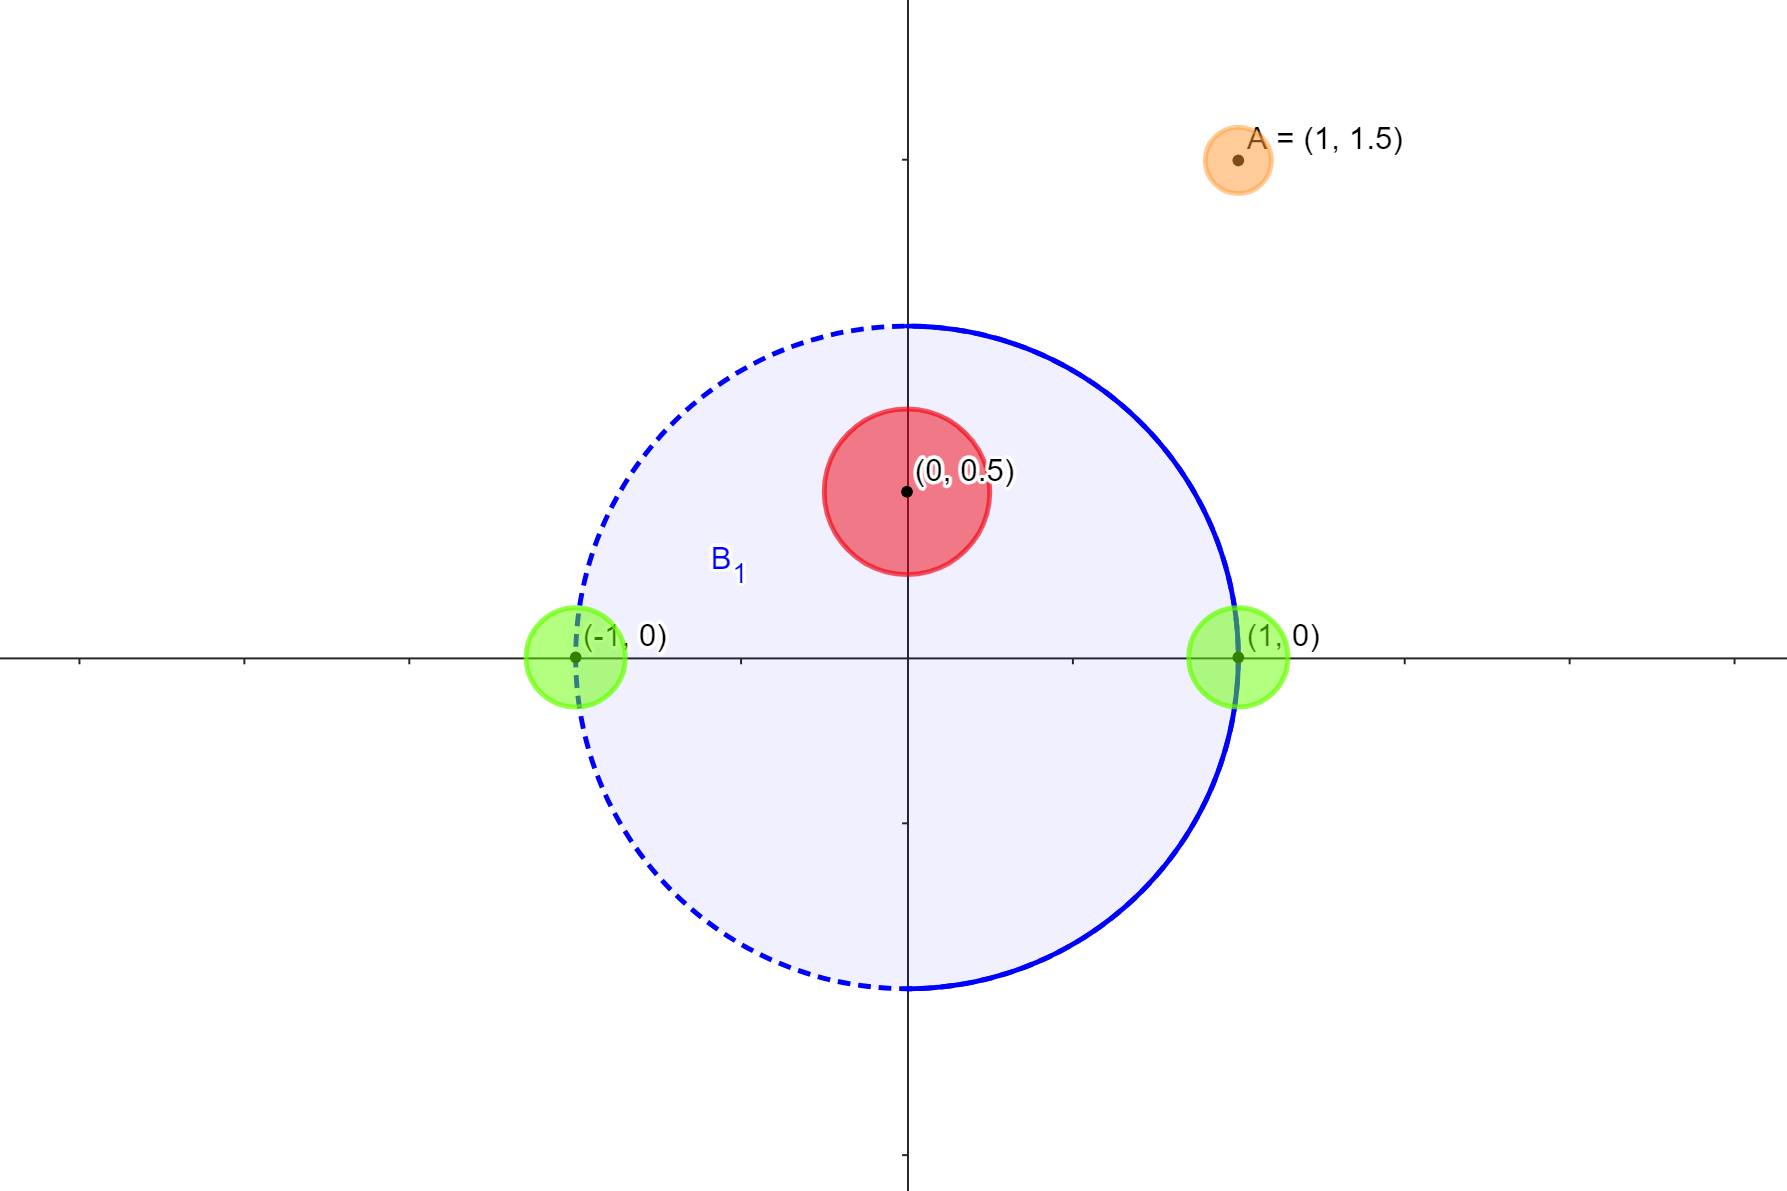
\includegraphics[width=\textwidth]{Capitoli/Capitolo2/Punti2.png}
    \end{minipage}
    \hfill
    \begin{minipage}{0.55\textwidth}  % Larghezza della minipage per il testo
        Si può dunque osservare che:
        \begin{itemize}
            \item $(0, \tfrac{1}{2})$ è \textit{interno}.
            \item $(1,0) $ è di \textit{frontiera} e di \textit{accumulazione}.
            \item $(-1,0) $ è di \textit{frontiera} e di \textit{accumulazione}.
            \item $(1, \tfrac{3}{2}) $ è di \textit{frontiera} e \textit{isolato}.
        \end{itemize}      
    \end{minipage}
\end{example}
\begin{definition}
    Un insieme $E \subseteq \mathbb{R}^n$ si dice \textbf{aperto} se
    \begin{equation}
        E=\mathring{E} \text{ oppure } E \cap \partial{E} = \emptyset
    \end{equation}
    ovvero se non ha punti esterni.
\end{definition}
\begin{definition}
    Si dice che un insieme $E \subseteq \mathbb{R}^n$ è \textbf{chiuso} se 
    \begin{equation}
        \partial{E} \subseteq E
    \end{equation}
    ovvero se $E^\complement$ è aperto.\\
    Si definisce poi \textbf{chiusura} di $E$ l'insieme
    \begin{equation}
        \overline{E} = E \cap \partial{E}
    \end{equation}
    Quindi un'altra definizione di insieme chiuso è:
    \begin{equation}
        E \text{ chiuso } \iff E=\overline{E}
    \end{equation}
\end{definition}
\begin{proposition}
    Un insieme $E$ è chiuso $\iff$ $E$ contiene tutti i suoi punti di accumulazione.
\end{proposition}
\begin{oss}
    $E=\{x_0\}$ con $x_0 \in \mathbb{R}^n$ fissato è chiuso e $E=\partial{E}$.
\end{oss}
\begin{oss}
    Dalla definizione, $\emptyset$ e $\mathbb{R}^n$ sono entrambi contemporaneamente aperti e chiusi e sono gli unici sottoinsiemi di $\mathbb{R}^n$ con tali proprietà.
\end{oss}
\begin{definition}
    Sia $E \subseteq \mathbb{R}^n$, $E$ si dice \textbf{limitato} se
    \begin{equation}
        \exists R>0 \text{ tale che } E \subseteq B_R(0)
    \end{equation}
    Altrimenti esso è detto \textbf{illimitato}.
\end{definition}
\begin{definition}
    Un insieme aperto $A\subseteq \mathbb{R}^n$ si dice \textbf{connesso} se non esistono due aperti $A_1, \ A_2$ non triviali (cioè diversi da $\emptyset,\ \mathbb{R}^n,\ A$) e disgiunti tali che
    \begin{equation}
        A=A_1 \cup A_2
    \end{equation}
\end{definition}
\begin{definition}
    Sia $E \subseteq \mathbb{R}^n$. Allora $E$ si dice \textbf{connesso per archi} se per ogni $(x,y) \in E$ esiste una curva parametrica $\varphi:[0,1] \to E$ tale che
    \begin{equation}
        \varphi(0)=x \land \varphi(1)=y
    \end{equation}
\end{definition}
\begin{definition}
   $E \subseteq \mathbb{R}^n$ si dice \textbf{dominio} (\textbf{connesso}) se è la chiusura di un aperto (connesso).
\end{definition}
\begin{definition}
    Un insieme $E \subseteq \mathbb{R}^n$ si dice \textbf{convesso} se, definito $[x,y]$ il segmento di estremi $x,\ y$ si ha che
    \begin{equation}
        [x,y] \subseteq E
    \end{equation}
    \begin{oss}
        Un insieme convesso è per definizione connesso per archi.
    \end{oss}
\end{definition}
\begin{definition}
    Un insieme $E \subseteq \mathbb{R}^n$ si dice \textbf{stellato} rispetto ad un punto $x_0$ di E se per ogni $x$ di $E$ si ha che
    \begin{equation}
        [x_0, x] \subseteq E
    \end{equation}
\end{definition}

%%  DEFINIZIONI SEQUENZIALI


\section{Definizioni sequenziali}
\begin{definition}
    Si dice \textbf{successione in $\mathbb{R}^n$} una funzione da $\mathbb{N}$ a valori in $\mathbb{R}^n$.
    \begin{equation}
        (x_k)_{k \in \mathbb{N}} = ((x_k)_1, \dots, (x_k)_n)  
    \end{equation}
    con $k \in \mathbb{N}$ indice intero della successione.
\end{definition}
\begin{definition}
    Sia $(x_k)_k$ una successione in $\mathbb{R}^n$. Si dice che $x_k$ \textbf{converge} a $\ell$, cioè
    \begin{equation}
        x_k \to \ell=(\ell_1, \dots, \ell_n) \in \mathbb{R}^n
    \end{equation}
    se la loro distanza converge a zero. Poiché 
    \begin{equation}
        d(x_k, \ell)=|x_k-\ell|=\sqrt{[(x_k)_1-\ell_1]^2+\dots+[(x_k)_n-\ell_n]^2}
    \end{equation}
    la successione converge se ogni sua componente converge a ciascuna componente di $\ell$, quindi
    \begin{equation}
        (x_k)_k \overset{k\to+\infty}{\to} \ell \iff (x_k)_i \overset{k\to+\infty}{\to} \ell_i \ \forall i
    \end{equation}
\end{definition}
\begin{definition}
    Sia $(x_k)_k$ una successione di vettori di $\mathbb{R}^n$. Si dice che $x_k$ \textbf{diverge} se
    \begin{equation}
        |x_k| \overset{k\to+\infty}{\to} \infty
    \end{equation}
    \begin{oss}
        Si osservi che è sufficiente che la norma di una sola componente di $x_k$ diverga affinché la successione sia divergente.
        \begin{example}
            Presa come successione $x_k=\left(\frac{1}{k}, k\right)$, poiché la sua seconda componente è divergente per $k \to \infty$, anche la successione lo è.
        \end{example}
    \end{oss}
\end{definition}
\begin{definition} \label{Def: Punto di accumulazione}
    Sia $E \subseteq \mathbb{R}^n$ e sia $x_0 \in \mathbb{R}^n$. Si dice che $x_0$ è \textbf{punto di accumulazione} per $E$ se
    \begin{equation}
        \exists\ (x_k)_k \text{ con } x_k\neq x_0 \in E \ \forall \ k \text{ tale che } x_k \to x_0
    \end{equation}
\end{definition}
\begin{definition}
    Sia $K \subseteq \mathbb{R}^n$. Si dice che $K$ è un insieme \textbf{compatto} se da ogni successione $(x_k)_k$ è possibile estrarre una sottosuccessione convergente ad un punto di $K$
\end{definition}
\begin{theorem}[Heine-Borel] \label{Teo: Heine Borel}
    Un insieme $K$ è compatto se e solo se è chiuso e limitato.
    \begin{oss}
        Un insieme $C \subseteq \mathbb{R}^n$ è chiuso se e solo se per ogni successione di elementi in $C$ convergente si ha che il limite di tale successione è contenuto in $C$.
    \end{oss}
\end{theorem}

%%  INTRODUZIONE FUNZIONI IN PIU VARIABILI

\section{Introduzione alle funzioni in più variabili}
Come già anticipato, da questo momento in avanti si studieranno prima le funzioni scalari e poi quelle a valori vettoriali.
Si cominci prima da alcune definizioni di carattere generale. 
\begin{definition}
    Si dice \textbf{dominio} di una funzione $f$ di $n$ variabili il più grande sottoinsieme di $\mathbb{R}^n$ su cui $f$ è definita. Esso viene indicato con $\text{dom}(f)$.
\end{definition}
\begin{definition}
    Sia $f: \Omega \subseteq \mathbb{R}^n \to \mathbb{R}$. Si dice \textbf{grafico} di $f$ il sottoinsieme di $mathbb{R}^{n+1}$
    \begin{equation}
        G(f)= \left\{(x_1, \dots, x_n, x_{n+1}) \in \Omega \times \mathbb{R} \mid x_{n+1}=f(x)\right\}
    \end{equation}
\end{definition}
\begin{definition}
    Sia $f:\Omega \subseteq \mathbb{R}^n \to \mathbb{R}$ e sia $l \in \mathbb{R}$. Si dice \textbf{superficie di livello} o \textbf{ipersuperficie} $l$ per $f$ il sottoinsieme
    \begin{equation}
        L_l=\left\{x \in \Omega \mid f(x)=l\right\}=f^{-1}(l)
    \end{equation}
\end{definition}

%%   LIMITI
\section{Limiti}
\begin{definition}[Limiti al finito] \label{Def: Limiti al finito}
    Sia $f:\Omega \subseteq \mathbb{R}^n \to \mathbb{R}$ e sia $x_0$ un punto di accumulazione per l'insieme $\Omega$.\\
    Si dice che $f$ \textbf{converge} a $\ell \in \mathbb{R}$ per $x \to x_0$ e si scrive
    \begin{equation}
        \lim_{x \to x_0}{f(x)}=\ell
    \end{equation} 
    se
    \begin{equation}
        \forall \varepsilon>0 \ \exists\delta=\delta_\varepsilon>0\ \text{tale che, se}\ 
                x \in B_\delta(x_0) \setminus \left\{x_0\right\}\ \cap\ \Omega
            \text{ allora}\ |f(x)-\ell|<\varepsilon
    \end{equation}
    Analogamente, si dice che $f$ \textbf{diverge} per $x \to x_0$ con $x \in \Omega$ e si scrive
    \begin{equation}
        \lim_{x \to x_0}{f(x)}=\underset{-\infty}{+\infty}
    \end{equation}
    se 
    \begin{equation}
        \forall M>0 \ \exists\delta=\delta_M>0\ \text{tale che, se}\ 
        x \in B_\delta(x_0) \setminus \left\{x_0\right\}\ \cap\ \Omega
            \text{ allora}\ \underset{f(x)<-M}{f(x)>M}
    \end{equation}
\end{definition}
\begin{definition}
    Sia $f:\Omega \subseteq \mathbb{R}^n$ con $x_0$ punto di accumulazione. Si dice che 
    \begin{equation}
        \lim_{x \to x_0}{f(x)}=\ell
    \end{equation}
    se per ogni successione di punti di $\Omega$ $(x_k)_k$ diversi da $x_0$ tali che
    \begin{equation}
        f(x_k)\to \ell
    \end{equation}
    \begin{oss}
        La definizione è analoga per i casi in cui $\ell$ sia infinito.
    \end{oss}
    \begin{oss}
        Stando alla definizione \ref{Def: Punto di accumulazione}, l'ipotesi di di $x_0$ punto di accumulazione garantisce l'esistenza di almeno una successione convergente.
    \end{oss}
\end{definition}
\begin{definition}[Limiti all'infinito] \label{Def: Limiti all'infinito}
    Sia $f:\Omega \to \mathbb{R}$. Allora, 
    \begin{equation}
        \lim_{x \to \infty}{f(x)}=\ell
    \end{equation}
    se
    \begin{equation}
        \forall \varepsilon > 0 \ \exists k=k_\varepsilon>0 \ \text{tale che, se}\ |x|>k_\varepsilon,\ \text{allora}\ |f(x)-\ell|<\varepsilon
    \end{equation}
    Analogamente,
    \begin{equation}
        \lim_{x \to \infty}{f(x)}=\underset{-\infty}{+\infty}
    \end{equation}
    se 
    \begin{equation}
        \forall M>0 \exists k=k_M>0 \ \text{tale che, se}\ |x|>k_M\ \text{allora}\ \underset{f(x)<-M}{f(x)>M}
    \end{equation}
\end{definition}
\subsection{Metodi per la risoluzione di limiti}
Il discorso che segue parte dal caso specifico di funzioni in due variabili ma può essere generalizzato con le dovute accortezze al caso di funzioni in $n$ variabili.\\
Si parta dallo specificare che anche per i limiti di funzioni multivariabile è possibile utilizzare le approssimazioni asintotiche.\\
Stando alla definizione di limite, esso non deve dipendere da come ci si avvicina a $x_0$. In prima istanza occorre allora scegliere uno degli innumerevoli metodi per farlo, noti come restrizioni. Tramite questi, è possibile trovare un candidato limite la cui esistenza deve essere verificata in uno dei modi che verranno illustrati.\\
Si può osservare che, se la funzione tende ad un limite $\ell$, allora esso è unico e valgono i teoremi delle funzioni in una variabile su somme, prodotti e quozienti di limiti; inoltre, se il limite esiste, $f$ tende (e deve tendere) a $\ell$ lungo ogni sua possibile restrizione. Viceversa, se esistono almeno due restrizioni il cui limite sia differente, il limite non esiste.\\
L'approccio per trovare il candidato limite ammette
\begin{itemize}
    \item Restrizioni lungo grafici di funzioni di $x$ o $y$ passanti per $(x_0, y_0)$ e appartenenti al dominio di $f$. In tal caso le funzioni possono essere $y= \varphi(x)$ o $x=\psi(y)$ e si avrà
    \begin{equation}
    \lim_{x \to x_0} f(x, \varphi(x)) \text{ o } \lim_{y \to y_0}{f(\psi(y), y)}
    \end{equation}
    \item Restrizioni lungo successioni $(x_n, y_n) \to (x_0, y_0)$ e in tal caso si calcola
    \begin{equation}
        \lim_{n \to +\infty}{f(x_n,y_n)}
    \end{equation}
    \item Restrizioni lungo curve parametriche $(x(t), y(t)): I \to \mathbb{R}^2$ passanti per $(x_0, y_0)$. In tal caso si calcola
    \begin{equation}
        \lim_{t \to t_0}{f(x(t), y(t))}
    \end{equation}
\end{itemize}
Si mostrino di seguito alcuni modi per provare l'esistenza del limite.
\paragraph{Definizione}
Per conseguire il risultato prefissato occorre maggiorare o minorare la funzione in maniera tale da trovare un $\delta_\varepsilon$ per cui la definizione di limite sia verificata.
\begin{example}
    Si mostri il procedimento sul seguente limite.
    \begin{equation*}
        \lim_{(x,y) \to (0,0)}x
    \end{equation*}
    Attraverso la restrizione $(0,y)$ si può osservare che il candidato limite è $0$. Ora occorre provare che ciò sia vero.
    Dunque bisogna capire se sia possibile trovare un $\delta$ dipendente da $\varepsilon$ per cui sotto l'ipotesi
    \begin{equation*}
        \begin{cases}
            0<|(x,y)-(0,0)|<\delta\\
            (x,y) \in \text{dom}f
        \end{cases}
    \end{equation*}
    si abbia $|x-0|<\varepsilon$.\\
    Fissato $\varepsilon$ e sapendo che $|x|=\sqrt{x^2+y^2}<\delta$, serve provare che $|x|<\varepsilon$. Ciò è vero scegliendo $\delta<\varepsilon$.\\
    Al contrario, preso qualsiasi altro valore di $\ell$ la definizione non è verificata, come ci si aspetta.
\end{example}
\paragraph{Confronto}
Così come avveniva nelle funzioni a una variabile, è possibile verificare un candidato limite maggiorandolo e minorandolo con funzioni convergenti al medesimo candidato limite, applicando, cioè, il metodo del confronto.
\begin{example}
    Si calcoli il limite seguente.
    \begin{equation*}
        \lim_{(x,y) \to (0,0)}{\frac{xy}{\sqrt{x^2+y^2}}}
    \end{equation*}
    Tramite la restrizione su uno dei due assi si ottiene $0$ come candidato limite.
    Siccome vale la disuguaglianza di Young, che afferma che 
    \begin{equation*}
        xy \leq \frac{x^2+y^2}{2}
    \end{equation*}
    si può verificare che
    \begin{equation*}
        0 \leq \left|\frac{xy}{\sqrt{x^2+y^2}}\right| \leq \frac{\sqrt{x^2+y^2}}{2}
    \end{equation*}
    con gli estremi convergenti a $0$. Pertanto, il limite esiste ed è $0$.
\end{example}
\paragraph{Coordinate polari}
Dal momento che per provare la definizione di limite si deve controllare una distanza, può essere utile passare alle coordinate polari centrate nel punto $(x_0, y_0)$, ottenendo
\begin{equation}
    \begin{cases}
        x=x_0+ \varrho \cos(\theta)\\
        y=y_0+ \varrho \sin(\theta)
    \end{cases}
\end{equation}
Così facendo, fissato $\theta$ e fatto convergere $\varrho \to 0^+$, il limite diventa
\begin{equation}
    \lim_{\varrho\to 0}{f(x_0+\varrho\cos(\theta), y_0+\varrho\sin(\theta))}=\ell
\end{equation}
Si consegue così una condizione necessaria per l'esistenza del limite. È tuttavia possibile estendere tale affermazione ad una condizione necessaria e sufficiente ricercando un criterio tale da rendere il risultato univocamente determinato da $\varrho$ (e valido così $\forall\ \theta$).
\begin{theorem} \label{Teo: Condizione necessaria e sufficiente per un limite}
    Sia $f(x,y): E \subseteq \mathbb{R}^2 \to \mathbb{R}$ e sia $(x_0, y_0)$ punto di accumulazione per $\text{dom}f$ e sia $\ell \in \mathbb{R}$. Allora esiste
    \begin{equation}
        \lim_{(x,y)\to(x_0, y_0)}f(x,y)=\ell
    \end{equation}
    se e solo se esistono $r>0$ e $g:(0, r) \to \mathbb{R}$ tali che
    \begin{equation}
        \lim_{\varrho \to 0^+}{g(\varrho)=0}
    \end{equation}
    e, per ogni $\theta \in [0, 2\pi],\ \varrho\in (0, r)$ si ha che 
    \begin{equation}
        \left|f(x_0+\varrho\cos(\theta), y_0+\varrho\sin(\theta))-\ell \right|\leq g(\varrho)
    \end{equation}
\end{theorem}
\begin{example}
    Si calcoli nuovamente questo limite.
    \begin{equation*}
        \lim_{(x, y) \to (0,0)}{\frac{xy}{\sqrt{x^2+y^2}}}
    \end{equation*}
    Come prima, il candidato limite è $0$.\\
    Applicando un cambio di coordinate si ha che
    \begin{equation*}
        \begin{cases}
            x=\varrho\cos(\theta)\\
            y=\varrho\sin(\theta)
        \end{cases}
    \end{equation*}
    e, dunque, $f$ diviene
    \begin{equation*}
        f(\varrho\cos(\theta),\varrho\sin(\theta))=\frac{\varrho^2\cos(\theta)\sin(\theta)}{\varrho}=\varrho\cos(\theta)\sin(\theta)
    \end{equation*}
    Di conseguenza,
    \begin{equation*}
        |f(\varrho\cos(\theta),\varrho\sin(\theta))- \ell|=\varrho\cos(\theta)\sin(\theta) \leq \varrho = g(\varrho)
    \end{equation*}
    Pertanto, il limite esiste ed è verificato.
\end{example}
\begin{example}
    Si fornisca ora un esempio di limite non definito.
    \begin{equation*}
        \lim_{(x,y) \to (0,0)}{\frac{xy}{x^2+y^2}}
    \end{equation*}
    Per dimostrare l'inesistenza di $\ell$ si può procedere innanzitutto sfruttando le restrizioni. Infatti, se prendendo come cammini gli assi, il candidato limite è $0$, prendendo una retta generica della forma $y=mx$ tale risultato non è comprovato.
    \begin{equation*}
        \lim_{(x, mx) \to (0,0)}{\frac{x^2m}{x^2+x^2m^2}}=\lim_{(x, mx) \to (0,0)}{\frac{m}{m^2+1}} \neq 0
    \end{equation*}
    In alternativa, si può verificare ciò con il teorema \ref{Teo: Condizione necessaria e sufficiente per un limite}. In coordinate polari il limite diviene
    \begin{equation*}
        \lim_{\varrho \to 0^+}{\left|\frac{\varrho^2\cos(\theta)\sin(\theta)}{\varrho^2}\right|}=\lim_{\varrho \to 0^+}{\left|\cos(\theta)\sin(\theta)\right|} < \frac{1}{2}=g(\varrho)
    \end{equation*}
    Ma $g(\varrho)$ non tende a $0$ per $\varrho \to 0^+$ quindi, il limite si riconferma indefinito.
\end{example}
\subsection{Continuità}
Si sfruttino ora le nozioni apprese sui limiti per definire la continuità di una funzione.
\begin{definition} \label{Def: Continuità}
    Sia $f: E \subseteq \mathbb{R}^n \to \mathbb{R}$ e sia $x_0 \in \mathbb{R}^n$. Se $x_0$ è un punto isolato di E, la funzione si dice \textbf{continua} in $x_0$ per convenzione. Se $x_0$ è di accumulazione per E, f è \textbf{continua} in $x_0$ se è definita in tale punto e
    \begin{equation} \label{Eq: Continuità}
        \lim_{x \to x_0} f(x)= f(x_0)
    \end{equation}
    ovvero, in termini di $\varepsilon$ e $\delta$, se
    \begin{equation}
        \forall \varepsilon > 0 \  \exists \delta>0 \text{ tale che se } x \in B_\delta(x_0) \cap E, \ |f(x)-f(x_0)|< \varepsilon
    \end{equation} 
    \begin{oss}
        Se f non è definita in $x_0$ ma esiste il limite $\ell$ di $f(x)$ per $x \to x_0$, è possibile definire il \textbf{prolungamento di continuità} per $f$ in $x_0$ come:
        \begin{equation}
            g(x) = \begin{cases}
                f(x) \text{ se } x \neq x_0, x \in \text{dom}f\\
                \ell \text { se } x=x_0
            \end{cases}
        \end{equation}
    \end{oss}
    \begin{oss}
        Rientrano tra le funzioni continue somme, prodotti, quozienti (ben definiti) di polinomi
    \end{oss}
\end{definition}
\vspace*{\baselineskip}
Si noti che anche per funzioni in più variabili continue vale un analogo del teorema di \textbf{permanenza del segno}, che afferma che, se $f$ è definita in $B_\delta(x_0)$ ed è continua in $x_0$ con $f(x_0) \gtrless 0$, allora esiste $B_\delta'(x_0)$ con $\delta' \leq \delta$ su cui il segno viene mantenuto.
\begin{definition}
Sia $f:X \subseteq \mathbb{R}^n \to \mathbb{R}$. Si dice che $x_0 \in X$ è \textbf{punto di massimo assoluto} (forte) per $f$ in $X$ se
\begin{equation}
    \begin{aligned}
        f(x) \leq f(x_0) \ \forall x  \in X \\
        (f(x) < f(x_0) \ \forall x  \in X)
    \end{aligned}
\end{equation}
In tal caso, $f(x_0)$ è detto \textbf{valore massimo} di $f$ su $X$.\\
In maniera del tutto analoga, data $f:X \subseteq \mathbb{R}^n \to \mathbb{R}$, si dice che $x_0 \in X$ è \textbf{punto di minimo assoluto} (forte) per $f$ in $X$ se
\begin{equation}
    \begin{aligned}
        f(x) \geq f(x_0) \ \forall x \in X\\
        (f(x)>f(x_0) \ \forall x \in X)
    \end{aligned}
\end{equation}
In tal caso, $f(x_0)$ è detto \textbf{valore minimo} di $f$ su $X$
\end{definition}
\begin{theorem}[Weierstrass] \label{Teo: Weierstrass}
    Sia $K \subseteq \mathbb{R}^n$ compatto e sia $f: K \to \mathbb{R}$ continua su $K$. Allora, esistono $x_m, x_M$ tali che
    \begin{equation}
    \min_{x \in K}{f(x)}= f(x_m) \leq f(x) \leq f(x_M) = \max_{x \in K}{f(x)}    
    \end{equation}
    \begin{oss}
        Una possibile notazione di min e max è $ \min_{K}{f}$ e $\max_{K}{f}$.
    \end{oss}
\end{theorem}
\begin{theorem}[Valori intermedi] \label{Teo: Valori intermedi}
    Sia $D \subseteq \mathbb{R}^n$ un dominio connesso (cioè la chiusura di un aperto connesso) e limitato. Allora $D$ è compatto per il teorema \ref{Teo: Heine Borel}.
    Sia poi $f:D \to \mathbb{R}$ continua su $D$. Allora $f$ assume su $D$ tutti i valori compresi tra $\min_{D}{f}$ e $\max_{D}{f}$ cioè
    \begin{equation}
        f(D)=\left[ \min_{D}{f}, \max_{D}{f}\right]
    \end{equation}
    \begin{oss}
        Se $D$ non è limitato, si ragiona su $\sup_{D}{f}$ e $\inf_{D}{f}$ anziché in termini di massimo e minimo.
    \end{oss}
\end{theorem}
\begin{corollary}[Teorema degli zeri] \label{Teo: Teorema degli zeri}
    Sia $f$ tale da rispettare le ipotesi del teorema \ref{Teo: Valori intermedi}. Siano poi $x_0, x_1 \in D$ tali che 
    \begin{equation}
        f(x_0)f(x_1) < 0
    \end{equation}
    allora, esiste $x^* \in D$ tale che $f(x^*)=0$.
\end{corollary}
\begin{definition} \label{Def: Uniforme continuità}
    Sia $f:E \subseteq \mathbb{R}^n \to \mathbb{R}$. Allora $f$ si dice \textbf{uniformemente continua} se
    \begin{equation}
        \forall \varepsilon >0 \ \exists \delta=\delta_\varepsilon\ \text{tale che}\ \forall x, y \in E\ \text{tali che}\ |x-y|<\delta\ \text{si ha che}\ |f(x)-f(y)| < \varepsilon
    \end{equation}
\end{definition}
\begin{theorem}[Heine Cantor] \label{Teo: Heine Cantor}
    Sia $f: K \subseteq \mathbb{R}^n \to \mathbb{R}$ continua con $K$ compatto. Allora $f$ è uniformemente continua su $K$.
\end{theorem}
Il teorema appena enunciato offre un metodo per verificare l'uniforme continuità su un compatto. Tuttavia, la definizione si applica su insiemi generici. Un metodo per verificare tale proprietà su insiemi non compatti è sfruttare la nozione di \textbf{lipschitzianità}.
\begin{definition}
    Sia $f:E \subseteq \mathbb{R}^n \to \mathbb{R}$. Si dice che $f$ è \textbf{lipschitziana} su $E$ con costante di Lipschitz $L>0$ se
    \begin{equation}
        \forall x,y \in E\ \text{si ha che}\ |f(x)-f(y)| \leq L|x-y|
    \end{equation}
\end{definition}
\begin{proposition}
    Le funzioni lipschitziane su $E$ sono uniformemente continue.
    \begin{proof}
        Si applichi ad una funzione lipschitziana la definizione di uniforme continuità con 
        \begin{equation}
            \delta= \frac{\varepsilon}{L}
        \end{equation}
    \end{proof}
\end{proposition}
Se il discorso sulla continuità dovesse riguardare una funzione a valori vettoriali $f: \mathbb{R}^n \to \mathbb{R}^m$ con $m>1$ anziché scalari, le definizioni di limite e continuità rimangono valide a patto che le condizioni siano verificate componente per componente, cioè
\begin{equation}
    \lim_{x \to x_0}{f(x)}=\ell \in \mathbb{R}^m \iff \lim_{x \to x_0}{f_i(x)}=\ell_i\ \forall i=1, \dots, m
\end{equation}
\section{Derivate direzionali}
Si passi ora alla trattazione del calcolo di derivate per funzioni multivariabile. Per fare ciò occorre prima definire cosa sia una \textit{direzione}.
\begin{definition} \label{Def: Direzione}
    Si dice \textbf{direzione} un vettore $v \in \mathbb{R}^n$ tale che abbia norma unitaria. 
\end{definition}
Fatto ciò, si può iniziare a parlare effettivamente di derivate direzionali, ovvero dello studio della derivata di una funzione in più variabili lungo una determinata direzione.
\begin{definition}
    Sia $f: A \subseteq \mathbb{R}^n \to \mathbb{R}$ e sia $x_0 \in A$. Sia poi $v \in \mathbb{R}^n$ una direzione fissata.
    Si dice allora che $f$ è \textbf{derivabile} in $x_0$ lungo la direzione $v$ se esiste \textit{finito}
    \begin{equation}
        \lim_{t \to 0}{\frac{f(x_0+tv)-f(x_0)}{t}}= \ell
    \end{equation}
    che viene detto \textbf{derivata direzionale} di $f$ in $x_0$ lungo la direzione $v$ e viene annotato con 
    \begin{equation}
        \frac{\partial{f}}{\partial{v}}(x_0)
    \end{equation}
\begin{oss}
    È possibile mostrare l'equivalenza di questa definizione con quella delle funzioni in una variabile. Infatti, definita una generica
    \begin{equation}
        g(t)=f(x_0+tv)
    \end{equation}
    si ha che 
    \begin{equation}
        \frac{\partial{f}}{\partial{v}}(x_0) = \lim_{t \to 0}{\frac{f(x_0+tv)-f(x_0)}{t}} = \lim_{t \to 0}{\frac{g(t+0)-g(0)}{t}}=g'(0)
    \end{equation}
\end{oss}
\end{definition}
\subsection{Derivate parziali}
Poiché esistono infinite direzioni, esistono altrettante derivate direzionali. Tra queste, dunque, occorre evidenziare $n$ direzioni privilegiate, ovvero i versori della base canonica $\mathcal{C}=\left\{e_1,\dots, e_n\right\}$. Lungo tali direzioni si hanno quindi le \textit{derivate parziali}.
\begin{definition} \label{Def: Derivate parziali}
    Si dicono \textbf{derivate parziali} le $n$ derivate in $x_0$ lungo un versore della base canonica e le si indica con
    \begin{equation}
        \frac{\partial{f}}{\partial{x_i}}
    \end{equation}
    dove con $x_i$ si mette in evidenza il fatto che la direzione sia privilegiata.
\end{definition}
La definizione di derivata parziale è dunque un caso particolare della derivata direzionale. La definizione di quest'ultima può essere rimodellata sulla prima così:
\begin{equation}
    \frac{\partial{f}}{\partial{x_i}}=\lim_{t \to 0}{\frac{f(x_0^1, \dots, x_0^i+t, \dots, x_0^n)-f(x_0^1, \dots, x_0^i, \dots, x_0^n)}{t}}
\end{equation}
Definite le direzioni privilegiate e le derivate parziali, si può ora formalizzare il concetto di derivabilità in un punto.
\begin{definition} \label{Def: Derivabilità}
    Sia $f:A \subseteq \mathbb{R}^n \to \mathbb{R}$ con $A$ aperto e sia $x_0 \in A$. Si dice che $f$ è \textbf{derivabile in $x_0$} se esistono finite le $n$ derivate parziali
    \begin{equation}
        \frac{\partial{f}}{\partial{x_i}}(x_0)
    \end{equation}
In tal caso si può definire un vettore di derivate in $x_0$. Tale vettore è detto \textbf{gradiente} e viene indicato con
\begin{equation}
    \nabla f(x_0) := \left(\frac{\partial{f}}{\partial{x_1}}(x_0), \dots, \frac{\partial{f}}{\partial{x_i}}(x_0), \dots, \frac{\partial{f}}{\partial{x_n}}(x_0)\right)\ \text{con}\ i \in [0,n]
\end{equation}
\end{definition}
Spesso il calcolo di una derivata parziale si riduce all'applicazione degli stessi metodi di differenziazione propri del calcolo differenziale di funzioni in una variabile con l'accortezza di considerare le altre variabili come costanti. Tuttavia non sempre è possibile farlo e occorre derivare tramite la definizione. Si mostrino alcuni esempi.
\begin{example}
    Sia $f(x, y)=xe^y$ e si voglia calcolare le due derivate parziali nel punto $(1,0)$.
    In generale le derivate parziali sono:
    \begin{equation*}
        \begin{aligned}
            \frac{\partial{f}}{\partial{x}}(x_0,y_0)=e^y \\
            \frac{\partial{f}}{\partial{x}}(x_0,y_0)=xe^y
        \end{aligned}
    \end{equation*}
    Quindi in $(1,0)$ si ha $\nabla f((1,0))=(1,1)$.
\end{example}
\begin{example}
    Sia $f(x,y)= yx^{\tfrac{2}{3}}$ e $(x_0, y_0)=(0,0)$.
    Allora,
    \begin{equation*}
        \frac{\partial{f}}{\partial{x}}(x_0,y_0)= \frac{2}{3}yx^{-\tfrac{1}{3}} \Big|_{(0,0)}
    \end{equation*}
    Tuttavia, la funzione non è di classe $C^1$ quindi bisogna usare la definizione.
    \begin{equation*}
        \frac{\partial{f}}{\partial{x}}(0,0)=\lim_{t \to 0}{\frac{f(t,0)-f(0,0)}{t}}=\lim_{t \to 0}{\frac{0-0}{t}}=0
    \end{equation*}
\end{example}
\begin{example}
    Sia $f(x,y)$ definita a tratti come segue
    \begin{equation*}
        f(x,y)= \begin{cases}
            \frac{xy^2}{x^2+y^4}\ &\text{se}\ (x,y)\neq (0,0)\\
            0\ &\text{se}\ (x,y)=(0,0)
        \end{cases}
    \end{equation*}
   e se ne calcolino le derivate direzionali in $(0,0)$.\\
   Non essendo la funzione continua, bisogna utilizzare la definizione.
   Si scelga allora come direzione un generico $v=(\cos(\alpha), \sin(\alpha))$.
   Quindi
   \begin{equation*}
    \begin{aligned}
        \frac{\partial{f}}{\partial{v}}(0,0)&=\lim_{t \to 0}{\frac{f((0,0)+t(\cos(\alpha), \sin(\alpha)))-f(0,0)}{t}}=\\
        &=\lim_{t \to 0}{\frac{f(t\cos(\alpha), t\sin(\alpha))}{t}}= \lim_{t \to 0}{\frac{\frac{t^3\cos(\alpha)\sin^2(\alpha)}{t^2\cos^2(\alpha)+t^4\sin^4(\alpha)}}{t}}=\\
        &=\lim_{t \to 0}{\frac{\cos(\alpha)\sin^2(\alpha)}{\cos^2(\alpha)+t^2\sin^4(\alpha)}}= \begin{cases}
            \frac{\sin^2(\alpha)}{\cos(\alpha)} &\text{se}\ \cos(\alpha) \neq 0\\
            0 & \text{se}\ \cos(\alpha)=0
        \end{cases}
    \end{aligned}
   \end{equation*}
   Dunque la funzione è derivabile in $(0,0)$ in ogni direzione pur non essendo ivi continua. Si mostri ora che la funzione non è continua in tale punto.
   Scegliendo come restrizione uno dei due assi, il candidato limite è $0$.\\
   Si prenda ora una generica retta $x=my$.
   \begin{equation*}
    \lim_{y \to 0}{\frac{my^3}{m^2y^2+y^4}} \sim \lim_{y \to 0}{\frac{y^3}{y^2}}=\lim_{y\to0}{y}=0
   \end{equation*}
   come ci si aspetterebbe.
   Applicando ora la restrizione $x=my^2$,
   \begin{equation*}
    \lim_{y \to 0}{\frac{my^4}{m^2y^4+y^4}}=\lim_{y \to 0}{\frac{my^4}{y^4(m^2+1)}}=\frac{m}{m^2+1} \neq 0
   \end{equation*}
   Pertanto, $f$ non è continua in $(0,0)$.
\end{example}
\begin{oss}
    Diversamente da quanto visto nelle funzioni in una variabile, è possibile osservare che in funzioni in più variabili la derivabilità (e la derivabilità in tutte le direzioni) non implicano la continuità della funzione.\\
    In maniera invece analoga, la continuità non implica la derivabilità di $f$.
\end{oss}
\subsection{Differenziabilità}
Se nello studio di funzioni monovariabile era possibile dimostrare che una funzione è derivabile se e solo se è differenziabile, in questo caso ciò non è più assicurato.
\begin{definition} \label{Def: Differenziabilità}
    Sia $f:A \subseteq \mathbb{R}^n \to \mathbb{R}$ con $A$ aperto e sia $x_0 \in A$. Si dice che $f$ è \textbf{differenziabile} in $x_0$ se esiste $\nu=(\nu_1, \nu_n) \in \mathbb{R}^n$ tale che
    \begin{equation}
        \lim_{x \to x_0}{\frac{f(x)-f(x_0)-\langle \nu, x-x_0\rangle}{|x-x_0|}}=0
    \end{equation}
\end{definition}
\begin{definition} {\label{Def: Piano tangente}}
    Sia $f:A \subseteq \mathbb{R}^n$ differenziabile in $x_0 \in A$. Allora si dice \textbf{iperpiano tangente} al grafico di $f$ in $(x_0, f(x_0))$ l'iperpiano di equazione
    \begin{equation}
        x_{n+1}= f(x_0)+ \langle \nabla f(x_0), x-x_0 \rangle
    \end{equation}
 \begin{oss}
    In $\mathbb{R}^2$, preso come punto $(x_0, y_0)$ allora il piano tangente ha equazione
    \begin{equation}
        z=f(x_0, y_0)+ \frac{\partial f }{\partial x}{(x_0, y_0)}(x-x_0) +\frac{\partial f }{\partial y}{(x_0, y_0)}(y-y_0) 
    \end{equation}
    e il versore normale è il normalizzato di
    \begin{equation}
        \left(-\frac{\partial f}{\partial x}{(x_0, y_0)}, -\frac{\partial f}{\partial y}{(x_0, y_0)},1\right)
    \end{equation}
 \end{oss}
\end{definition}
\begin{proposition} \label{Prop: Diff-Der-Cont}
    Sia $f:A \to \mathbb{R}$ differenziabile in $x_0 \in A$. Allora:
    \begin{enumerate}
        \item $f$ è continua in $x_0$
        \item $f$ è derivabile in $x_0$ e $\nu=\nabla f(x_0)$
        \item $f$ è derivabile in ogni direzione in $x_0$ e vale la \textit{formula del gradiente}
            \begin{equation} \label{Eq:Formula gradiente}
                \frac{\partial{f}}{\partial{v}}(x_0)= \langle \nabla f(x_0), v\rangle
            \end{equation}
    \end{enumerate}
    \begin{proof}
        Si dimostri il primo fatto. La tesi è
        \begin{equation}
            \lim_{h \to 0}{f(x_0+h)}=f(x_0)
        \end{equation}
        Dall'ipotesi di differenziabilità si sa che
        \begin{equation}
            f(x_0+h)-f(x_0)-\langle \nu, h \rangle = o(|h|)\ \text{per}\ h \to 0
        \end{equation}
        Tramite la disuguaglianza di Cauchy-Schwarz per la norma
        \begin{equation} \label{Eq: Cauchy-Schwarz}
            | \langle \underline{v}, \underline{w} \rangle | \leq |\underline{v}||\underline{w}|
        \end{equation}
        si ha che 
        \begin{equation}
            \lim_{h \to 0}{f(x_0+h)}= \lim_{h \to 0} {f(x_0)+ \langle \nu, h \rangle + o(|h|)}\overset{\substack{\ref{Eq: Cauchy-Schwarz}\\ \text{su $\langle \nu, h \rangle$}}}{=} f(x_0)
        \end{equation}
        Si dimostri ora la seconda tesi, cioè che 
        \begin{equation}
            \nu=(\nu_1, \dots, \nu_n)= \nabla f(x_0) = \left(\frac{\partial{f}}{\partial{x_1}}{(x_0)}, \dots, \frac{\partial{f}}{\partial{x_n}}{(x_0)}\right)
        \end{equation}
        Sia $i \in [1, n]$ fissato. La definizione di derivata parziale è
        \begin{equation}
            \begin{aligned}
               \frac{\partial{f}}{\partial{x_i}}(x_0)&=\lim_{t \to 0}{\frac{f(x_0+te_i)-f(x_0)}{t}}=\lim_{t \to 0}{\frac{f(x_0+te_i)-f(x_0)-t\nu_i+t\nu_i}{t}}=\\
               &=\lim_{t \to 0}{\frac{f(x_0+te_i)-f(x_0)-t\nu_i}{t} \frac{|t|}{|t|}}+\lim_{t \to 0}{\frac{t\nu_i}{t}}\overset{\substack{\text{Diff. sul}\\\text{primo}}}{=} \nu_i
            \end{aligned}
        \end{equation}
        Di conseguenza, poiché $\forall\ \nu_i$, $\nu_i=\frac{\partial{f}}{\partial{x_i}}(x_0)$, se $f$ è differenziabile in $x_0$ allora è anche derivabile in $x_0$ e $\nabla f(x_0)$ coincide con il vettore $\nu$.\\
        Infine, si dimostri il terzo fatto, cioè che, presa $f$ differenziabile allora essa è derivabile in ogni direzione e vale
        \begin{equation}
            \frac{\partial{f}}{\partial{v}}(x_0)=\langle \nabla f(x_0), v\rangle
        \end{equation}
        Si parta dalla definizione di differenziabilità con $h=tv$, con $v$ direzione.
        \begin{equation}
            \lim_{t \to 0} {\frac{f(x_0+tv)-f(x_0)-\langle \nabla f (x_0), tv \rangle}{|t|}}=0
        \end{equation}
        Si scriva poi la definizione di derivata direzionale
        \begin{equation}
            \frac{\partial f}{\partial v}(x_0)= \lim_{t \to 0}{\frac{f(x_0+tv)- f(x_0)}{t}}
        \end{equation}
        Allora aggiungendo e togliendo $\langle \nabla f (x_0), tv \rangle$ si può notare che
        \begin{equation}
            \begin{aligned}
                \frac{\partial f}{\partial v}(x_0)&= \lim_{t \to 0}{\frac{f(x_0+tv)- f(x_0) -\langle \nabla f (x_0), tv \rangle+ \langle \nabla f (x_0), tv \rangle}{t}}=\\
                &\overset{\text{Linearità}}{=} \lim_{t \to 0}{\frac{f(x_0+tv)- f(x_0) -\langle \nabla f (x_0), tv \rangle}{t} \frac{|t|}{|t|}} + \lim_{t \to 0}{\frac{t \langle \nabla f (x_0), v \rangle}{t}}=\\
                &\overset{\substack{\text{Diff. sul}\\\text{primo}}}{=} \langle \nabla f (x_0), v \rangle
            \end{aligned}
        \end{equation}
    \end{proof}
\end{proposition}
\begin{proposition}[Direzioni di massima e minima crescita] \label{Prop: Interpretazione geometrica del gradiente}
    Sia $f: A \subseteq \mathbb{R}^n \to \mathbb{R}$ e sia $x_0 \in A$. Se $f$ è differenziabile e $\nabla f(x_0) \neq 0$, allora
    \begin{equation}
        \begin{aligned}
            &\max_{v \in \mathbb{R}^n,\ |v|=1}{\frac{\partial f}{\partial v}{(x_0)}}=\frac{\partial f}{\partial v_M}(x_0)=|\nabla f(x_0)|\ \text{con}\ v_M= \frac{\nabla f(x_0)}{|\nabla f(x_0)|}\\
            &\min_{v \in \mathbb{R}^n,\ |v|=1}{\frac{\partial f}{\partial v}{(x_0)}}=\frac{\partial f}{\partial v_m}(x_0)=-|\nabla f(x_0)|\ \text{con}\ v_m= -v_M
        \end{aligned}
    \end{equation}
    \begin{proof}
        Poiché $f$ è differenziabile, si può sfruttare la formula del gradiente. Inoltre, applicando anche la disuguaglianza di Cauchy-Schwarz è possibile dire che
       \begin{equation}
        \left|\frac{\partial f}{\partial v}(x_0)\right|= \left|\langle \nabla f(x_0), v\rangle\right| \leq \left|\nabla f(x_0)\right| \left|v\right|
       \end{equation}
       Quindi, essendo $v$ un versore, si ha che 
       \begin{equation}
        - \left|\nabla f(x_0)\right| \leq \frac{\partial f}{\partial v}(x_0) \leq \left|\nabla f(x_0)\right|
       \end{equation}
       Se poi $\nabla f(x_0) \neq 0$ e $v=v_M$, si ha
       \begin{equation}
        \frac{\partial f }{\partial v_M}= \langle \nabla f(x_0), v_M\rangle = \langle \nabla f(x_0), \frac{\nabla f (x_0)}{|\nabla f(x_0)|}\rangle=\frac{|\nabla f(x_0)|^2}{|\nabla f(x_0)|}=|\nabla f(x_0)|
       \end{equation}
       Il discorso è analogo nel caso $v=v_m$.
    \end{proof}
\end{proposition}
\begin{theorem}[Differenziale totale] \label{Teo: Differenziale totale}
    Sia $f:A \subseteq \mathbb{R}^n \to \mathbb{R}$ e sia $x_0 \in A$. Se $f$ è derivabile in $A$ e se le derivate parziali $f_{x_i}$ sono continue in $x_0$ $\forall i=1, \dots, n$, allora $f$ è differenziabile in $x_0$.
    \begin{proof}
        Senza perdita di generalità, si dimostri il teorema in dimensione $n=2$. Occorre mostrare che $f(x,y)$ è differenziabile in $(x_0, y_0)$, cioè
        \begin{equation} \label{Eq: Difftot 1}
            \lim_{(h,k) \to (0,0)} \frac{f(x_0+h, y_0+k)-f(x_0, y_0)-\langle\nabla f(x_0, y_0), (h,k)\rangle}{\sqrt{h^2+k^2}}=0
        \end{equation}
        Per fare ciò si osservi che
        \begin{equation} \label{Eq: Difftot 2}
            \begin{aligned}
                f(x_0+h, y_0+k)-f(x_0, y_0)=&f(x_0+h, y_0+k)-f(x_0, y_0+k)\\&+f(x_0, y_0+k)-f(x_0, y_0)
            \end{aligned}
        \end{equation}
        Essendo $f$ derivabile in $A$, si può applicare il teorema di Lagrange alle funzioni:
        \begin{equation}
            x \mapsto f(x, y_0+k) \hspace{1.5cm} y \mapsto f(x_0, y)
        \end{equation}
        negli intervalli $[x_0, x_0+h]$ e $[y_0, y_0+h]$ con $h,k>0$ (altrimenti si scambiano gli estremi).
        Di conseguenza, esistono $x_1 \in [x_0, x_0+h] $ e $y_1 \in [y_0, y_0+h]$ tali che
        \begin{equation}
            \begin{cases}
                f_x(x_1, y_0+k)h=\left[f(x_0+h, y_0+k)-f(x_0, y_0+k)\right]\\
                f_y(x_0, y_1)k=\left[f(x_0, y_0+k)-f(x_0, y_0) \right]
            \end{cases}
        \end{equation}
        Sostituendo nella \eqref{Eq: Difftot 2} si ottiene che
        \begin{equation} \label{Eq: Difftot 3}
            f(x_0+h, y_0+k)-f(x_0, y_0)=f_x(x_1, y_0+k)h+f_y(x_0, y_0+k)k
        \end{equation}
        Pertanto, risolvendo il prodotto scalare della \eqref{Eq: Difftot 1}, si ha che
        \begin{equation}
            \begin{aligned}
                &\frac{|f(x_0+h, y_0+k)-f(x_0, y_0)-f_x(x_0, y_0)h-f_y(x_0, y_0)k|}{\sqrt{h^2+k^2}}=\\
                &\overset{\eqref{Eq: Difftot 3}}{=}\frac{|f_x(x_1, y_0+k)h-f_x(x_0, y_0)h+f_y(x_0, y_0+k)k-f_y(x_0, y_0)k|}{\sqrt{h^2+k^2}}\leq\\
                &\overset{\substack{\text{Triangolare,}\\\text{Schwarz}}}{\leq} \frac{|f_x(x_1, y_0+k)-f_x(x_0, y_0)||h|}{\sqrt{h^2+k^2}}+\frac{|f_y(x_0, y_0+k)-f_y(x_0, y_0)||k|}{\sqrt{h^2+k^2}}\leq\\
                &\overset{\text{Maggiorazione}}{\leq} |f_x(x_1, y_0+k)-f_x(x_0, y_0)|+|f_y(x_0, y_0+k)-f(x_0, y_0)|
            \end{aligned}
        \end{equation}
        Infatti, $\forall\ h,k \neq 0$ vale
        \begin{equation}
            \frac{|h|}{\sqrt{h^2+k^2}}\leq 1 \hspace{1.5 cm} \frac{|k|}{\sqrt{h^2+k^2}}\leq 1
        \end{equation}
        Allora per $(h,k) \to (0,0)$ si ha che $x_1 \to x_0$ e $y_1 \to y_0$. Essendo per ipotesi le derivate parziali continue in $(x_0, y_0)$, si ottiene
        \begin{equation}
            \begin{cases}
                f_x(x_1, y_0+k) \overset{(h, k) \to (0,0)}{\to} f_x(x_0, y_0)\\
                f_y(x_0, y_1) \overset{(h, k) \to (0,0)}{\to} f_y(x_0, y_0)
            \end{cases}
        \end{equation} 
        e quindi 
        \begin{equation}
            \frac{|f(x_0+h, y_0+k)-f(x_0, y_0)-f_x(x_0, y_0)h-f_y(x_0, y_0)k}{\sqrt{h^2+k^2}} \overset{(h,k)\to(0,0)}{\to} (0,0)
        \end{equation}
    \end{proof}
\end{theorem}
\begin{definition} \label{Def:C0 e C1}
    Si dice che $f:A \subseteq \mathbb{R}^n\to \mathbb{R}$ è di \textbf{classe $C^0$ in $A$} e lo si indica con $f \in C^0(A)$ se è continua su $A$.\\
    Se poi $f$ è derivabile in $A$ e le sue derivate parziali sono continue in $A$, allora $f$ è detta di \textbf{classe $C^1$ in $A$} e lo si indica con $f \in C^1(A)$.\\
    \begin{oss}
        Operando una sintesi tra i risultati ottenuti dalla proposizione \ref{Prop: Diff-Der-Cont}, dal teorema del differenziale totale (\ref{Teo: Differenziale totale}) e dalla definizione appena fornita, si può osservare che
        \begin{equation} \label{Eq: Relazione C^1 -> diff -> C^0}
            f \in C^1(A) \Rightarrow f\ \text{differenziabile in}\ A \Rightarrow f \in C^{0}(A)
        \end{equation}
    \end{oss} 
\end{definition}
\subsection{Derivate successive}
Terminata questa prima trattazione sulle derivate direzionali e la differenziabilità, si può progredire nel discorso introducendo le derivate successive.
\begin{definition}
    Sia $f:A \subseteq \mathbb{R}^n \to \mathbb{R}$ derivabile in A. Si dice che $f$ è \textbf{derivabile due volte} in $x_0 \in A$ se esistono finite tutte le derivate seconde in $x_0$, cioè se sono ben definite
    \begin{equation}
        \frac{\partial}{\partial x_j}\left(\frac{\partial f}{\partial x_i}\right)(x_0)=\frac{\partial^2f}{\partial x_j \partial x_i}(x_0)=f_{x_ix_j}
    \end{equation}
    Se poi ciò avviene su tutto $A$, $f$ si dice derivabile due volte su $A$.
\end{definition}
Si osservi che tutte le derivate seconde si ottengono non solo al variare di $i=1, \dots, n$ ma anche al variare di $j=1, \dots, n$. Pertanto, si parla di matrice delle derivate seconde o di \textbf{matrice hessiana}, indicata con $H_f$ e descritta da $H_f=(f_{x_ix_j})$ o, in maniera esplicita,
\begin{equation} \label{Eq: Matrice hessiana}
    H_f = \begin{pmatrix}
    \frac{\partial^2 f}{\partial x_1^2} & \frac{\partial^2 f}{\partial x_1 \partial x_2} & \dots  & \frac{\partial^2 f}{\partial x_1 \partial x_n} \\
    \frac{\partial^2 f}{\partial x_2 \partial x_1} & \frac{\partial^2 f}{\partial x_2^2}  & \dots  & \frac{\partial^2 f}{\partial x_2 \partial x_n} \\
    \vdots & \vdots & \ddots & \vdots \\
    \frac{\partial^2 f}{\partial x_n \partial x_1} & \frac{\partial^2 f}{\partial x_n \partial x_2} & \dots  & \frac{\partial^2 f}{\partial x_n^2}
    \end{pmatrix}
\end{equation}
In particolare, gli elementi della diagonale principale sono detti anche \textit{derivate seconde pure}, gli altri \textit{derivate seconde miste}.\\
Inoltre, di norma la matrice hessiana non è simmetrica. Tuttavia, è possibile stabilire delle condizioni sufficienti per la simmetria della stessa.
\begin{theorem}[Teorema di Schwarz] \label{Teo: Schwarz}
    Sia $A \subseteq \mathbb{R}^n$ aperto, sia $x_0 \in A$ e sia poi $f: A \to \mathbb{R}$ una funzione reale derivabile due volte in $x_0$. Allora, se $f_{x_ix_j}$ e $f_{x_jx_i}$ con $i \neq j$ sono funzioni continue, allora 
    \begin{equation}
        f_{x_ix_j}=f_{x_jx_i}
    \end{equation}
    \begin{example}
        Si consideri $f(x, y)=x e^x$. Allora, $\nabla f(x,y)=(e^y, xe^y)$.
        Pertanto, calcolandone le derivate parziali seconde si ottiene
        \begin{equation*}
            H_f=\begin{pmatrix}
                0 &e^y\\
                e^y &xe^y
            \end{pmatrix}
        \end{equation*}
        e, come previsto, tale matrice è simmetrica.
    \end{example}
    \begin{example}
        Si fornisca ora un esempio di funzione la cui matrice hessiana non sia simmetrica.\\
        Si prenda:
        \begin{equation*}
            f(x,y)=\begin{cases}
                xy \frac{x^2-y^2}{x^2+y^2} &\text{se}\ (x,y)\neq (0,0)\\
                0 &\text{se}\ (x,y)=(0,0)
            \end{cases}
        \end{equation*}
        Si può osservare che tale funzione è di classe $C1$ su $(0,0)$ e il suo gradiente è
        \begin{equation*}
            \begin{cases}
                \left(y \frac{x^2-y^2}{x^2+y^2}+\frac{4(x^2y^3)}{(x^2+y^2)^2},x \frac{x^2-y^2}{x^2+y^2}-\frac{4(y^2x^3)}{(x^2+y^2)^2}\right) &\text{se}\ (x,y)\neq(0,0)\\
                (0,0) &\text{se}\ (x,y)=(0,0)
            \end{cases}
        \end{equation*}
        Allora, si calcolino le derivate seconde miste in $(0,0)$
        \begin{equation*}
            \begin{aligned}
                &f_{xy}(0,0)=\lim_{k \to 0}\frac{f_x(0,k)-f_x(0,0)}{k}= \lim_{k\to 0}{\frac{1}{k} \frac{k(-k^2)}{k^2}}=-1\\
                &f_{yx}(0,0)=\lim_{h \to 0} \frac{f_y(h,0)-f_y(0,0)}{h}=\lim_{h \to 0}{\frac{1}{h} \frac{h(h^2)}{h^2}}=1
            \end{aligned}
        \end{equation*}
        Si può infatti osservare che la funzione $f$ cambia segno, cioè $f(x,y)=-f(y,x)$. Perciò le due derivate miste, che per tale asimmetria sono discontinue in $(0,0)$, non coincidono, come previsto dal teorema di Schwarz.
    \end{example}
\end{theorem}
Quanto detto nella definizione \ref{Def:C0 e C1} può essere generalizzato come segue.
\begin{definition} \label{Def: Ck}
    Sia $f:A \subseteq \mathbb{R}^n\to \mathbb{R}$ tale che abbia derivate parziali continue di ordine $k \in \mathbb{N}$ in $A$, allora, si dice che $f$ è di \textbf{classe $C^k(A)$} e lo si indica con $f \in C^k(A)$.
    In particolare, si definisce la \textbf{classe $C^\infty$} su $A$ come
    \begin{equation}
      C^\infty= \bigcap_{k \in \mathbb{N}}{C^k(A)}
    \end{equation}
\end{definition}
\begin{corollary}
    Se $f \in C^2(A)$, allora $H_f$ è simmetrica in ogni punto del dominio.
\end{corollary}
\begin{theorem}[Derivata della funzione composta 1] \label{Teo: Derivata composta 1}
    Sia $f:A \subseteq \mathbb{R}^n \to \mathbb{R}$ e sia $x: I \to \mathbb{R}$ una curva. Si assuma che $x(I) \subseteq A$. Se $x(t)=(x_1(t), \dots, x_n(t))$ è derivabile in ogni $x_i:I \to \mathbb{R}$, se $t_0 \in I$ e se $f$ differenziabile in $x(t_0)$, allora
    $f \circ x$ è derivabile in $t_0$ e vale
    \begin{equation}
        (f \circ x)'(t_0)= \langle \nabla f(x(t_0)), x'(t_0) \rangle \label{Eq: Derivata composta 1}
    \end{equation}
\begin{oss}
    L'ipotesi $x(I) \subseteq A$ serve a garantire una composizione ben definita.
\end{oss}
\end{theorem}
\begin{theorem}[Derivata della funzione composta 2] \label{Teo: Derivata composta 2}
    Sia $f:A \subseteq \mathbb{R}^n \to \mathbb{R}$ e sia $x: B \subseteq \mathbb{R}^k \to \mathbb{R}^n$ con $B$ aperto. Sia poi $F(y)=f(x(y))=(f \circ x): B \to \mathbb{R}$ con $y \in B$. Se $x_1 \dots x_n$ sono derivabili parzialmente (o $C^1$ o differenziabili) rispetto ad una certa $y_j$ fissata, e $f$ è differenziabile in $x(y_0) \in A$, allora $F$ è derivabile parzialmente (o $C^1$ o differenziabile) rispetto a $y_j$ e vale 
    \begin{equation} \label{Eq: Derivata composta 2}
        \frac{\partial f}{\partial y_j}=\left\langle \nabla f(x(y_0)), \frac{\partial x}{\partial y_j}(y_0)\right\rangle=\sum\limits_{i=1}^{n}{\frac{\partial f}{\partial x_i}(x(y_0))\ \frac{\partial x_i}{\partial y_j}(y_0)}
    \end{equation}    
\end{theorem}
\begin{proposition} \label{Prop: Premessa al teo Lagrange}
    Sia $f:A \subseteq \mathbb{R}^n \to \mathbb{R}$ tale che $f \in C^2(A)$. Siano poi $x_0 \in A$ e $h \in \mathbb{R}^n \setminus \left\{0\right\}$ tali che $\left[x_0, x_0+h\right] \subseteq A$. Sia poi $F(t)=f(x_0+th)$ con $t \in [0,1]$ e $F \in C^2([0,1])$. Allora, si ha che
    \begin{equation}
        \begin{aligned} \label{Eq: Premessa al teo Lagrange}
            &F'(t)=\sum\limits_{i=0}^{n}{\frac{\partial f}{\partial x_i}(x_0+th)h_i}\\ 
            &F''(t)=\langle H_f(x_0+th)h, h \rangle 
        \end{aligned}
    \end{equation}
    \begin{proof}
        Per dimostrare il primo fatto bisogna osservare che si è calcolata la derivata di una funzione composta secondo la formula \eqref{Eq: Derivata composta 2}.\\
        Si dimostri ora la seconda equazione.
        \begin{equation}
            \begin{aligned}
                F''(t)&= \frac{d}{dt}\left(\sum\limits_{i=1}^{n}{\frac{\partial f}{\partial x_i}(x_0+th)h_i}\right)\overset{\substack{\text{Prop.}\\\text{der.}}}{=}\sum\limits_{i=1}^{n}{h_i\frac{d}{dt}\left(\frac{\partial f}{\partial x_i}(x_0+th)\right)}=\\
                &\overset{\text{Comp.}}{=}\sum\limits_{i=1}^{n}h_i\left\langle\frac{\partial f}{\partial x_i}(x_0+th), h\right\rangle=\sum\limits_{i=1}^{n}h_i \sum\limits_{j=1}^{n}{\frac{\partial^2 f}{\partial x_j \partial x_i}(x_0+th)h_j}=\\
                &=\sum\limits_{i,j=1}^{n}{{\frac{\partial^2 f}{\partial x_j \partial x_i}(x_0+th)h_ih_j}}= \langle H_f(x_0+th)h,h\rangle 
            \end{aligned}
        \end{equation}
    \end{proof}
\end{proposition}
\begin{theorem}[Lagrange] \label{Teo: Lagrange}
    Sia $f: A \subseteq \mathbb{R}^n \to \mathbb{R}$ tale che $f \in C^1(A)$. Siano $x_0$ e $x_0+h \in A$ tali che $[x_0, x_0+h] \subseteq A$. Allora, $\exists\ \theta \in [0,1]$ tale che
    \begin{equation}
        f(x_0+h)-f(x_0)= \langle \nabla f(x_0+ \theta h), h \rangle
    \end{equation}
    \begin{proof}
        Sia $F$ definita come nella proposizione \ref{Prop: Premessa al teo Lagrange}. Allora il risultato discende dal teorema di Lagrange in una dimensione. Infatti, essendo $F$ derivabile in $[0,1]$ si ha che
        \begin{equation}
            F(1)-F(0)=f(x_0+h)-f(x_0)\overset{\text{Lag 1-d}}{=}F'(\theta)\overset{\eqref{Eq: Premessa al teo Lagrange}}{=}\langle \nabla f(x_0+ \theta h), h \rangle
        \end{equation}
        per un qualche $\theta \in [0,1]$.
    \end{proof} 
\end{theorem}
\begin{theorem}[Formula di Taylor con resto di Lagrange al II ordine] \label{Teo: Taylor con resto di Lagrange}
    Sia $f:A \subseteq \mathbb{R}^n \to \mathbb{R}$ tale che $f\in C^2(A)$ e siano $x_0,\ x_0+h \in A$ tali che $[x_0, x_0+h] \subseteq A$. Allora, $\exists\ \theta \in [0,1]$ tale che
    \begin{equation}
        f(x_0+h)=f(x_0)+ \langle \nabla f(x_0), h \rangle + \frac{1}{2}\langle H_f(x_0+\theta h),h \rangle 
    \end{equation} 
    \begin{proof}
        Si parta dal ricordare la struttura della formula di Taylor con resto di Lagrange per funzioni in una variabile:
        \begin{equation}
            f(x)=p_n(x)+R_n(x)
        \end{equation}
        con $p_n$ polinomio di Taylor di ordine $n$ e $R_n$ resto di Lagrange definiti come:
        \begin{equation}
            \begin{aligned}
                &p_n(x)=\sum\limits_{k=0}^{n}{\frac{f^{(k)}(x_0)}{k!}(x-x_0)^k}\\
                &R_n(x)=\frac{f^{(n+1)}(z)}{(n+1)!}(x-x_0)^{(n+1)}
            \end{aligned}
        \end{equation}
        Di conseguenza, definendo F come nella proposizione \ref{Prop: Premessa al teo Lagrange}. Poiché $F \in C^2$, la tesi segue dalla formula di Taylor mostrata sopra.
        Quindi, al secondo ordine, 
        \begin{equation}
            F(1)=F(0)+F'(0)+\frac{1}{2}F''(\theta)
        \end{equation}
        cioè, grazie ai calcoli svolti nella proposizione \ref{Prop: Premessa al teo Lagrange}, 
        \begin{equation}
            f(x_0+h)= f(x_0)+\langle \nabla f(x_0), h \rangle + \frac{1}{2}\langle H_f(x_0+ \theta h)h, h\rangle
        \end{equation}
    \end{proof}
\end{theorem}
\begin{theorem}[Formula di Taylor con resto di Peano al II ordine] \label{Teo: Taylor con resto di Peano}
    Sia $f: A \subseteq \mathbb{R}^n \to \mathbb{R}$ tale che $f \in C^2(A)$ e siano $x_0,\ x_0+h \in A$ tali che $[x_0, x_0+h] \subseteq A$. Allora, 
    \begin{equation}
        f(x_0+h)=f(x_0)+\langle \nabla f(x_0), h \rangle+ \frac{1}{2} \langle H_f(x_0)h, h\rangle + o(|h|^2),\ h \to 0 \label{Eq: Taylor con resto di Peano}
    \end{equation}
    \begin{proof}
        A partire dal teorema \ref{Teo: Taylor con resto di Lagrange}, si mostri che 
        \begin{equation}
            \langle H_f(x_0+\theta h)h, h \rangle = \langle H_f(x_0)h,h \rangle + o(|h|^2)
        \end{equation}
        cioè che 
        \begin{equation}
            \lim_{h\to 0}{\frac{\langle H_f(x_0+\theta h)h, h \rangle - \langle H_f(x_0)h, h \rangle}{|h|^2}}=0
        \end{equation}
        Si sfrutti innanzitutto il seguente lemma.
        \begin{lemma}
            Sia $M \in \mathbb{M}_{n,n}$ e sia $h \in \mathbb{R}^n$. Allora, come conseguenza della disuguaglianza di Cauchy-Schwarz, 
            \begin{equation}
                |Mh| \leq |M| |h|
            \end{equation}
            con 
            \begin{equation} \label{Eq: Norma di Frobenius}
                |M|=\sqrt{\sum\limits_{i,j=1}^{n}{m_{ij}^2}}
            \end{equation}
            Tale norma è detta norma di Frobenius.
        \end{lemma}
        In particolare si verifica che
        \begin{equation}
            \begin{aligned}
                &\frac{|\langle H_f(x_0+\theta h)h, h \rangle - \langle H_f(x_0)h, h\rangle|}{|h|^2}\leq\\
                &\overset{\substack{\text{Prop.}\\\text{prod.}\\ \text{scal.}}}{\leq}\frac{|\langle [H_f(x_0+\theta h)-H_f(x_0)]h, h \rangle|}{|h|^2} \leq\\
                &\overset{\substack{\text{Cauchy}\\\text{Schwarz}}}{\leq} \frac{|[H_f(x_0+\theta h)-H_f(x_0)]h|\ |h|}{|h|^2} \leq\\
                &\overset{\substack{\text{Cauchy}\\\text{Schwarz}}}{\leq} \frac{|H_f(x_0+\theta h)-H_f(x_0)|\ |h|}{|h|} =\\
                &\overset{f \in C^2(A)}{=}|H_f(x_0+\theta h)-H_f(x_0)| \overset{h \to 0}{\to} 0
            \end{aligned}
        \end{equation}
    \end{proof}
\end{theorem}
\subsection{Ottimizzazione libera (su aperti)}
\begin{definition} \label{Def: Max e min relativo}
    Sia $f:E \subseteq \mathbb{R}^n \to \mathbb{R}$ e sia $x_0 \in E$. Allora $x_0$ è detto \textbf{punto di massimo relativo (minimo relativo)} se
    \begin{equation}
        \exists\ B_\delta(x_0)\ \text{con}\ \delta>0\ \text{tale che}\ f(x) \underset{(\geq)}{\leq} f(x_0)\ \forall\ x \in E \cap B_\delta(x_0)
    \end{equation}
    In particolare, se $x_0$ è un massimo o un minimo, lo si dice \textbf{estremo relativo}.
\end{definition}
\begin{theorem}[Fermat o Condizione necessaria del I ordine]
Sia $f:A \subseteq \mathbb{R}^n  \to \mathbb{R}$ e $x_0 \in \mathring{A}$. Se $x_0$ è un punto di massimo o minimo relativo per $f$ e $f$ è derivabile in $x_0$, allora
\begin{equation}
    \nabla f(x_0)=0
\end{equation}
\begin{proof}
    Senza perdita di generalità si supponga di avere $x_0$ massimo relativo. Allora bisogna mostrare
    \begin{equation}
        \frac{\partial f}{\partial x_i}(x_0)=0\ \forall\ i=1, \dots, n
    \end{equation}
    Poiché $A$ è aperto, esiste $\delta>0$ tale che sia ben definita per ogni $t \in (-\delta, \delta)$
    \begin{equation}
        g_i(t)=f(x_0+t e_i)
    \end{equation}
    Inoltre, $g$ è derivabile in $t=0$ e, poiché $x_0$ è per ipotesi massimo relativo, 
    \begin{equation}
        g_i(t) \leq g_i(0)\ \forall t \in \mathcal{U}(0)
    \end{equation}
    Applicando il teorema di Fermat per le funzioni in una variabile si osserva che
    \begin{equation}
        0=g_i'(0)=\frac{\partial f}{\partial x_i}(x_0)\ \forall\ i=1, \dots, n
    \end{equation}
\end{proof}
\end{theorem}
\begin{definition} \label{Def: Insieme dei punti critici}
    Sia $A$ aperto e $f: A \subseteq \mathbb{R}^n  \to \mathbb{R}$ allora si dice \textbf{insieme dei punti critici} l'insieme definito da
    \begin{equation}
        \left\{x\in A \mid \nabla f(x)=0\right\}
    \end{equation}
\end{definition}
\begin{definition} \label{Def: Punto di sella}
    Sia $x_0$ un punto critico per $f:A \subseteq \mathbb{R}^n \to \mathbb{R}$. Se $x_0$ non è massimo o minimo relativo, allora è detto \textbf{punto di sella}, cioè
    \begin{equation}
        \forall\ B_\delta(x_0)\ \exists\ x,y \in B_\delta(x_0)\ \text{tale che}\ f(x)>f(x_0)>f(y)
    \end{equation} 
\end{definition}
\begin{example}
    Si facciano esempi di punti critici.
    \begin{figure}[H]
        \centering
        \begin{minipage}{0.26\textwidth}
            \centering
            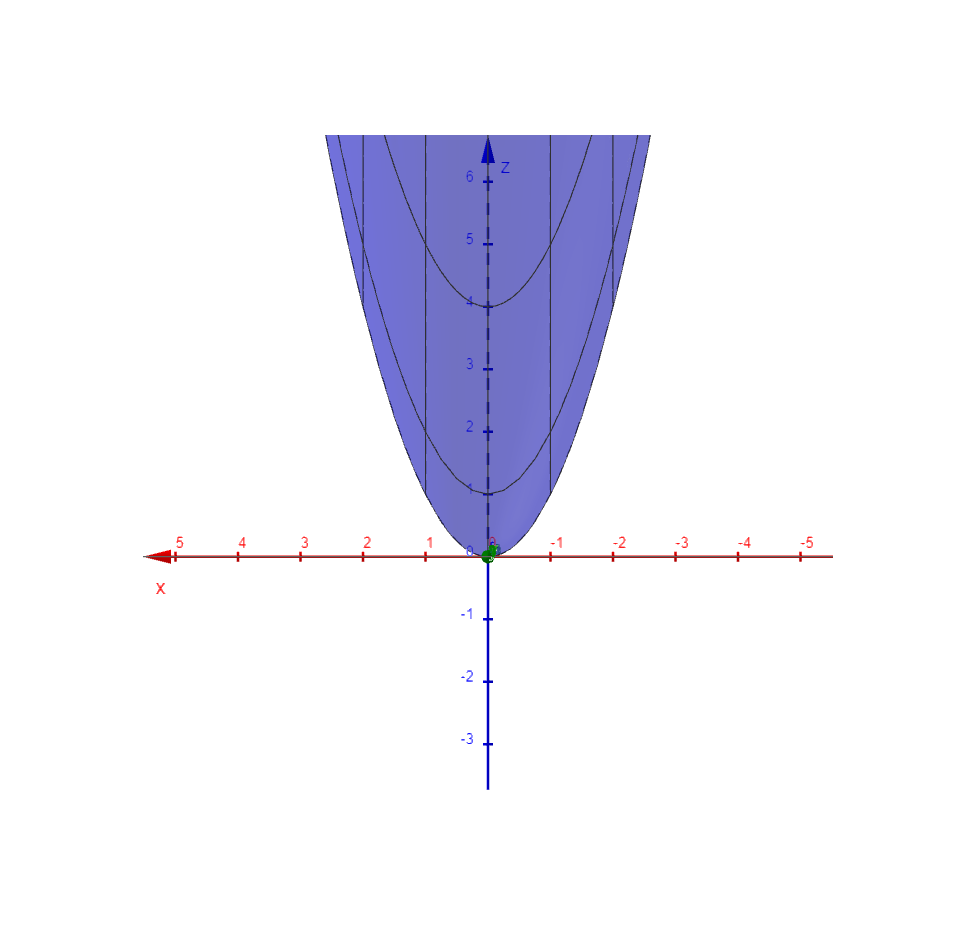
\includegraphics[width=\textwidth]{Capitoli/Capitolo2/Minimo.png}
            \caption{Grafico di $f(x,y)=x^2+y^2$ che mostra un minimo in $(0,0)$.}
        \end{minipage}
        \hspace{1cm}
        \begin{minipage}{0.26\textwidth}
            \centering
            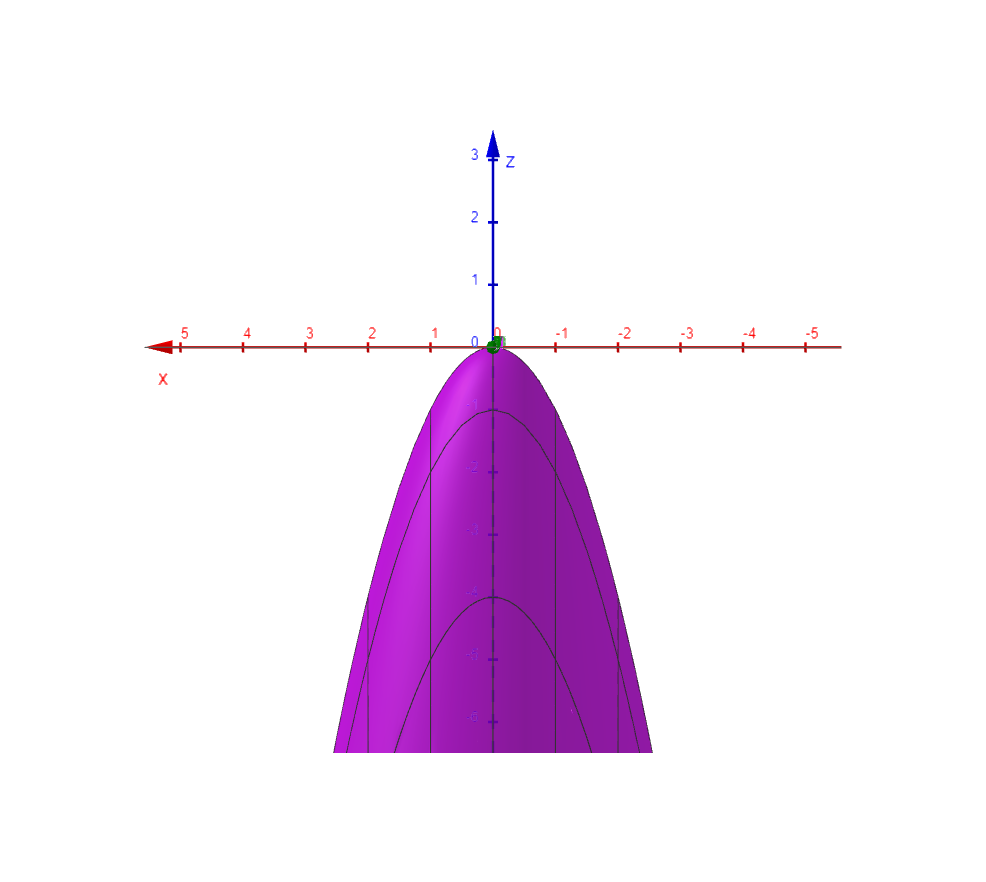
\includegraphics[width=\textwidth]{Capitoli/Capitolo2/Massimo.png}
            \caption{Grafico di $f(x,y)=-x^2-y^2$ che mostra un massimo in $(0,0)$.}
        \end{minipage}
        \hspace{1cm}
        \begin{minipage}{0.26\textwidth}
            \centering
            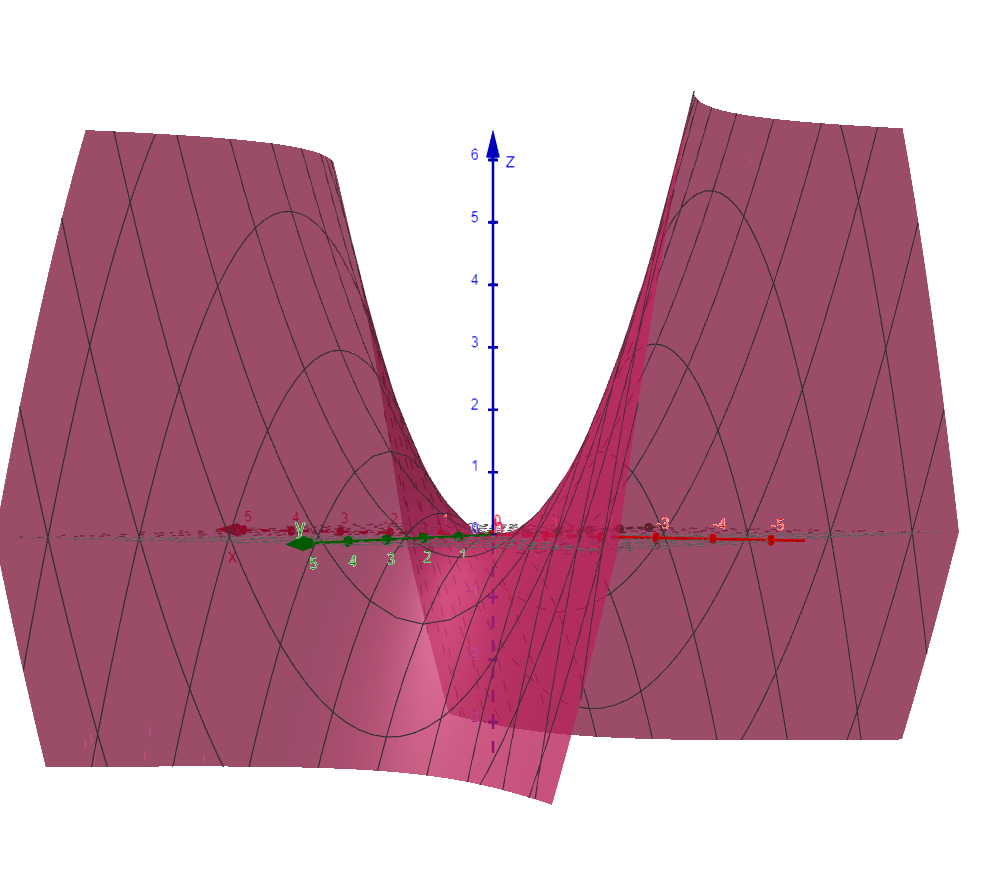
\includegraphics[width=\textwidth]{Capitoli/Capitolo2/Sella 3.png}
            \caption{Grafico di $f(x,y)=\frac{x^2}{3}-\frac{y^2}{3}$ che mostra punto di sella in $(0,0)$.}
        \end{minipage}
    \end{figure}
\end{example}
\paragraph{Richiami sulle forme quadratiche} Una \textbf{forma quadratica} è un polinomio omogeneo di secondo grado tale che
\begin{equation}
    q(\lambda x)=\lambda^2 q(x)\ \forall x \in \mathbb{R}^n,\ \lambda \in \mathbb{R}
\end{equation}
In particolare ad una forma quadratica può essere associata univocamente una matrice rappresentativa simmetrica definita come 
\begin{equation}
    Q=q_{ij}\ \text{con}\ q_{ij}=\frac{a_{ij}+a_{ji}}{2}
\end{equation}
tale che
\begin{equation}
    q(x)=\langle Qx, x \rangle
\end{equation}
\begin{oss}
    Si può notare come nel teorema di Taylor la forma $\langle H_f(x_0)h, h \rangle$ sia una forma quadratica \textit{indotta} da $H_f$.
\end{oss}
Inoltre, una forma quadratica può essere detta:
\begin{itemize}
    \item \textit{Definita positiva (negativa)} se $\forall\ \lambda_i$ si ha che $\lambda_i \underset{(<)}{>}0$
    \item \textit{Semidefinita positiva (negativa)} se $\forall\ \lambda_i$ si ha che $\lambda_i \underset{(\leq)}{\geq}0$
    \item \textit{Indefinita} se $\exists\ \lambda_i, \lambda_j$ tali che $\lambda_i\lambda_j<0$
\end{itemize}
\paragraph{Classificazione dei punti critici} Sia $x_0 \in A$ un punto critico per $f:A \subseteq \mathbb{R}^n\to \mathbb{R}$. Allora il polinomio di Taylor con resto di Peano al secondo ordine è
\begin{equation}
    \begin{aligned}
        f(x_0+h)&=f(x_0)+ \langle \nabla f(x_0), h\rangle+ \frac{1}{2}\langle H_f(x_0)h,h \rangle +o(|h|^2)=\\ 
        &= f(x_0)+ \frac{1}{2}\langle H_f(x_0)h,h \rangle + o(|h|^2)
    \end{aligned}
\end{equation} 
Quindi, per poter fornire dei criteri di classificazione dei punti critici occorre studiare il segno della forma quadratica indotta da $H_f$.
\begin{proposition}
    Sia $f:A \subseteq \mathbb{R}^n \to \mathbb{R}$ e sia $f \in C^2(A)$. Sia poi $x_0$ un punto critico per $f$.\\
    Se $x_0$ è un massimo relativo, allora $H_f(x_0)$ è (semi)definita negativa.
    \begin{equation}
        \langle H_f(x_0)h, h \rangle \underset{(\leq)}{<} 0
    \end{equation}
    Se $x_0$ è un minimo relativo, allora $H_f(x_0)$ è (semi)definita positiva.
    \begin{equation}
        \langle H_f(x_0)h, h \rangle \underset{(\geq)}{>} 0
    \end{equation}
\end{proposition}
\begin{theorem} [Condizione necessaria del II ordine] \label{Teo: Condizione necessaria del secondo ordine}
Sia $f: A \subseteq \mathbb{R}^n \to \mathbb{R}$ e sia $x_0 \in A$ critico per $f$. Sia poi $f \in C^2(A)$. Se $x_0$ è massimo (minimo) relativo, allora $H_f(x_0)$ è semidefinita negativa (positiva).
\begin{proof}
    Sia $x_0$ un punto di massimo relativo per $f$ , sia $v \in \mathbb{R}^n$ direzione fissata. Si definisca allora
    \begin{equation}
    F(t)=f(x_0+tv)
    \end{equation}
    Siccome $A$ è aperto, $F$ è definita su un certo $\left(-\delta, \delta\right)$ con $\delta>0$. Per ipotesi su $f$, $F$ ha un massimo relativo in $t=0$ ed è di classe $C^2(-\delta, +\delta)$.\\
    Per l'equazione \eqref{Eq: Premessa al teo Lagrange}, si ottiene che
    \begin{equation}
        F''(t)= \langle H_f(x_0+tv)v, v \rangle 
    \end{equation}
    da cui, per condizione necessaria sulle funzioni di una variabile, segue che
    \begin{equation}
        F''(0)= \langle (x_0)v, v \rangle \leq 0
    \end{equation}
    cioè che $H_f(x_0)$ è semidefinita negativa.\\
    La dimostrazione del caso in cui $x_0$ è minimo relativo per $f$ è del tutto analoga.
\end{proof}
\end{theorem}
\begin{lemma} \label{Lemma: FQ di matrice simmetrica è compresa tra i suoi autovalori max e min}
        Se, presa $A \in \mathbb{M}_{n,n}$ simmetrica e detti $\lambda_1 \leq \lambda_2 \leq \lambda_n$ i suoi autovalori, si ha $\langle Ax, x \rangle$, allora $\lambda_1 |x| \leq \langle Ax, x \rangle \leq \lambda_n |x|$
\end{lemma}
\begin{theorem}[Condizione sufficiente del II ordine] \label{Teo: Condizione sufficiente del secondo ordine}
    Sia $f:A \subseteq \mathbb{R}^n \to \mathbb{R}$ e sia $f \in C^2(A)$. Sia poi $x_0$ un punto critico per $f$. Allora, 
    \begin{itemize}
        \item Se $H_f(x_0)$ è definita positiva (negativa), allora $x_0$ è un minimo (massimo) relativo.
        \item Se $H_f(x_0)$ è indefinita, allora $x_0$ è un punto di sella.
    \end{itemize}
    \begin{proof}
        Si consideri il caso in cui $H_f(x_0)$ sia definita positiva e si mostri che $x_0$ è un punto di minimo per $f$\\
        Si può osservare che, essendo $H_f \in C^2(A)$, allora essa è simmetrica per il teorema \ref{Teo: Schwarz} e vale dunque il lemma \ref{Lemma: FQ di matrice simmetrica è compresa tra i suoi autovalori max e min}. Pertanto, indicato con $\lambda_{min}>0$ il minor autovalore di $H_f$, si ha che
        \begin{equation}
            \langle H_f(x_0)h,h \rangle \geq \lambda_{min} |h|^2\ \forall h \in \mathbb{R}^n
        \end{equation}
        Si scriva quindi lo sviluppo di Taylor con resto di Peano al secondo ordine in $f(x_0)$.
        \begin{equation}
        \begin{aligned}
            f(x_0+h)-f(x_0)&= \langle \nabla f(x_0), h \rangle + \frac{1}{2}\langle H_f(x_0h, h\rangle + o(|h|^2)=\\
            &\overset{f'(x_0)=0}{=} \frac{1}{2}\langle H_f(x_0)h, h\rangle + o(|h|^2) \geq \\
            &\overset{\text{Lemma}\ \ref{Lemma: FQ di matrice simmetrica è compresa tra i suoi autovalori max e min}}{\geq} \frac{1}{2} \lambda_{min}|h|^2+o(|h|^2)
        \end{aligned}
        \end{equation}
        Poiché scopo della dimostrazione è mostrare che $f(x_0+h)-f(x_0) \geq 0\ \forall h \in \mathbb{R}^n$, occorre provare che $o(|h|^2)$ sia trascurabile.
        \begin{equation}
            f(x_0+h)- f(x_0) \geq \frac{1}{2}\lambda_{min} |h|^2 \left( 1 + \frac{o(|h|^2}{\tfrac{1}{2}\lambda_{min}|h|^2}\right)
        \end{equation}
        ma, per definizione di o-piccolo vale il seguente fatto:
        \begin{equation}
            \exists\ \sigma >0\ \text{tale che, se}\ |h|<\sigma\ \text{allora}\ \frac{o(|h|^2}{\tfrac{1}{2}\lambda_{min} |h|^2} < \frac{1}{2}
        \end{equation}
        dove $\sigma=\frac{1}{2}$ è una costante arbitraria in $(0,1)$.
        Per tale disuguaglianza, allora, 
        \begin{equation}
        \begin{aligned}
            f(x_0+h)-f(x_0)&\geq \frac{1}{2}\lambda_{min} |h|^2 \left( 1 + \frac{o(|h|^2}{\tfrac{1}{2}\lambda_{min}|h|^2}\right) \geq \\
            &\geq \frac{1}{2}\lambda_{min}|h|^2(1-\frac{1}{2})=\frac{1}{4}\lambda_{min}|h|^2 >0
            \end{aligned}
        \end{equation}
        purché $|h|< \sigma$. In tal caso la definizione di minimo è soddisfatta.\\
        La dimostrazione per $H_f(x_0)$ definita negativa è analoga.\\
    Si dimostri ora il punto 2.\\
    Se $H_f(x_0)$ è indefinita, allora non soddisfa le ipotesi della condizione necessaria del secondo ordine (teorema \ref{Teo: Condizione necessaria del secondo ordine}), cioè non è né massimo né minimo. Quindi, essendo per ipotesi critico, deve essere una sella.
    \end{proof}
    \begin{oss}
        Se vale $f(x_0+h)-f(x_0) \gtrless 0$, $x_0$ si dice minimo (massimo) forte.
    \end{oss}
    \begin{oss}
        Si noti che non è possibile concludere niente previa indagine nel caso in cui $H_f$ sia semidefinita.
    \end{oss}
\end{theorem}
    \paragraph{Metodo delle restrizioni} Come accennato, se $H_f(x_0)$ è semidefinita, non è possibile caratterizzare il punto critico. Si mostri allora un metodo per farlo tramite esempio.
    \begin{example}
        Sia $f(x,y)=x^4-y^4$. Allora il punto $(0,0)$ è critico e si ha che
        \begin{equation*}
            H_f(0,0)=\begin{pmatrix}
                0 & 0\\
                0 & 0
            \end{pmatrix}
        \end{equation*}
        con $f(0,0)=0$. Si può osservare, però che:
        \begin{equation*}
            \begin{aligned}
                &f(x, 0) > 0\ \forall x \neq 0\\
                &f(0,y) < 0 \ \forall y \neq 0
            \end{aligned}
        \end{equation*}
        Pertanto $(0,0)$ è un punto di sella, giacché non è né un massimo né un minimo.
    \end{example}
    Può capitare, però, di non trovare restrizioni di quel genere, allora bisogna ricorrere allo studio del segno di
    \begin{equation*}
        f(x)-f(x_0)
    \end{equation*}
\section{Funzioni a valori vettoriali}
\begin{definition} \label{Def: Funzioni a valori vettoriali}
    Siano $n,\ m \in \mathbb{N}$ e sia $A \subseteq \mathbb{R}^n$. Allora si dice che una funzione $f$ è \textbf{a valori vettoriali} se è così definita:
    \begin{equation}
    \begin{aligned}
        f:A \subseteq \mathbb{R}^n &\to \mathbb{R}^m\\
        (x_1, \dots, x_n) &\mapsto (f_1(x_1, \dots, x_n), \dots, f_n(x_1, \dots, x_n))
    \end{aligned}
    \end{equation}
\begin{oss}
    Si noti che limiti, continuità e derivabilità vanno estese ad un ragionamento componente per componente.
\end{oss}
\begin{oss}
    Se la dimensione del dominio e del codominio è la medesima, si parla di \textit{campo vettoriale}.
\end{oss}
\end{definition}
\begin{definition} \label{Def: Derivabilità di f. vettoriali}
    Si dice che $f:A \subseteq \mathbb{R}^n \to \mathbb{R}^m$ è \textbf{derivabile} in $x_0 \in A$ se ciascuna $f_i$ con $i=1, \dots, n$ è ivi derivabile.
\end{definition}
\begin{definition} \label{Def: Matrice Jacobiana}
    Se $f$ è derivabile in $x_0$, si dice \textbf{matrice jacobiana} di $f$ in $x_0$ la matrice $J_f \in \mathbb{M}_{m,n}$ definita da
    \begin{equation} \label{Eq: Matrice Jacobiana}
        J_f(x_0)=\begin{pmatrix}
            \frac{\partial{f_1}}{\partial{x_1}}(x_0) & \frac{\partial{f_1}}{\partial{x_2}}(x_0)& \dots & \frac{\partial{f_1}}{\partial{x_n}}(x_0)\\
            \frac{\partial{f_2}}{\partial{x_1}}(x_0)& \frac{\partial{f_2}}{\partial{x_2}}(x_0)& \dots & \frac{\partial{f_2}}{\partial{x_n}}(x_0)\\
            \vdots & \vdots & \ddots & \vdots\\
            \frac{\partial{f_n}}{\partial{x_1}}(x_0) & \frac{\partial{f_n}}{x_2}(x_0)& \dots & \frac{\partial{f_n}}{\partial{x_n}}(x_0)
        \end{pmatrix}
        =
        \begin{pmatrix}
            \nabla f_1 (x_0)\\
            \nabla f_2(x_0)\\
            \vdots\\
            \nabla f_n(x_0)
        \end{pmatrix}
    \end{equation}
\end{definition}
\begin{definition} \label{Def: Differenziabilità di f. vettoriali}
    Una funzione $f$ si dice \textbf{differenziabile} in $x_0 \in A$ se
    \begin{equation}
        \lim_{h \to 0}{\frac{f(x_0+h)-f(x_0)-J_f(x_0)h}{|h|}}=0
    \end{equation}
\end{definition}
\begin{theorem} \label{Teo: Derivata composta di f. vettoriali}
Siano $g: B \subseteq \mathbb{R}^k \to A \subseteq R^n$ e $f: A \subseteq \mathbb{R}^n \to \mathbb{R}^m$ e le si assuma di classe $C^1$. Allora, $h=f \circ g: B \to \mathbb{R^m}$ è ben definita su $B$, è di classe $C^1(B)$ e vale:
\begin{equation}
    J_h(y) \in \mathbb{M}_{m,n}\ \text{tale che}\ J_h(y)=J_f(g(y)) J_g(y)\ \forall\ y \in B
\end{equation}
\begin{oss}
    Essendo di classe $C^1$, $h$ è differenziabile, in accordo con i ragionamenti già svolti nell'equazione \eqref{Eq: Relazione C^1 -> diff -> C^0}.
\end{oss}
\end{theorem}\cleardoublepage
\chapter{Funzioni implicite}
Può spesso capitare di avere a che fare con insiemi di $\mathbb{R}^2$ descritti da
\begin{equation} \label{Eq: Insieme implicito}
    F(x,y)=0 
\end{equation}
e detti \textbf{impliciti}.\\
L'obiettivo del capitolo è quello di trovare le condizioni sotto le quali la \eqref{Eq: Insieme implicito} permetta di associare ad $x$ un unico valore di $y$ come funzione di $x$,  arrivando a determinare le condizioni di esistenza di un intervallo $I \subseteq \mathbb{R}^n$ e di una funzione $f: I \to \mathbb{R}$ tale che
\begin{equation} \label{Eq: Scopo capitolo 3}
    F(x, f(x))=0 \qquad \forall\ x \in I
\end{equation}
Prima di procedere nella trattazione, si forniscano alcune definizioni di base utili nel corso del capitolo.
\begin{definition} \label{Def: Funzione implicita}
    Siano $I \subseteq \mathbb{R}^2,\ J \subseteq \mathbb{R}$ tali che
    \begin{equation}
        \forall\ x\in I\ \exists!\ y \in J\ \text{tale che}\ F(x,y)=0
    \end{equation}
    Allora si dice che l'equazione $F(x,y)=0$ \textbf{definisce implicitamente} una funzione $f: I \to J$.
\end{definition}
\begin{definition} \label{Def: Insieme degli zeri}
    Si dice \textbf{insieme degli zeri} della funzione $F$ l'insieme $Z(F)$ così definito:
    \begin{equation} \label{Eq: Insieme degli zeri}
        Z(F)=\left\{(x,y) \in I \mid F(x, y)=0 \right\}
    \end{equation}
\end{definition}
\begin{definition}
    Sia $Z(F)$ definito come nella \eqref{Eq: Insieme degli zeri} e sia $P=(\overline{x}, \overline{y}) \in Z(F)$. Se $\nabla F(\overline{x}, \overline{y})\neq 0$, si dice che $P$ è un \textbf{punto regolare} di $Z(F)$. Altrimenti $P$ è un \textbf{punto singolare}.
\end{definition}
\section{Teorema del Dini}
Il teorema del Dini, che verrà affrontato di seguito, fornisce le condizioni sotto le quali l'equazione $F(x,y)=0$ esprime $y$ in funzione di $x$ per certi valori delle variabili $x$, $y$.
\newpage
\begin{theorem}[Teorema del Dini] \label{Teo: Teorema del Dini}
    Sia $F: A \subseteq \mathbb{R}^2 \to \mathbb{R}$, $A$ aperto, una funzione continua in A e tale che
    \begin{equation}
    \exists\ \frac{\partial{F}}{\partial{y}} \in A 
    \end{equation}
    ed essa sia ivi continua. Inoltre, preso $(x_0, y_0) \in A$, se 
    \begin{equation}
    (x_0, y_0) \in Z(F) \quad \text{e} \quad \frac{\partial{F}}{\partial{y}}(x_0, y_0) \neq 0
    \end{equation}
    Allora, l'equazione
    \begin{equation}
        F(x, y)=0
    \end{equation}
    definisce implicitamente un'unica funzione
    \begin{equation}
        g: (x_0-\delta, x_0+\delta) \to (y_0 - \sigma, y_0+\sigma)
    \end{equation}
    tale che 
    \begin{equation} \label{Eq: Tesi Dini}
     y=g(x) \iff
        \begin{cases}
            F(x, y)=0\\
            x \in (x_0-\delta, x_0+\delta)\\
            y \in (y_0 - \sigma, y_0+\sigma)
        \end{cases} 
    \end{equation}
    Inoltre $g$ è continua in $(x_0-\delta, x_0+\delta)$ e $g(x_0)=y_0$
\end{theorem}
\begin{proof}
        Si supponga $\frac{\partial{F}}{\partial{y}}(x_0,y_0) > 0$. Poiché per ipotesi essa è anche continua, per permanenza del segno si ha che $\exists\ \sigma > 0$ tale che
        \begin{equation}
            \frac{\partial{F}}{\partial{y}}(x,y) > 0 \quad \forall\ (x,y) \in [x_0-\sigma, x_0+\sigma]\times [y_0 - \sigma, y_0+\sigma]
        \end{equation}
       Sia $x_0$ fissato. Definita $\eta(y)=F(x_0, y)$ si ha che
       \begin{equation}
           \eta'(y)=\frac{\partial{F}}{\partial{y}}(x_0, y) >0 \quad \forall\ y \in [y_0 - \sigma, y_0+\sigma]
       \end{equation}
       Pertanto $\eta(y)$ è continua, strettamente crescente e nulla in $y_0$. Quindi
       \begin{equation}
       \begin{aligned}
           &\eta(y_0-\sigma)=F(x_0, y_0-\sigma)<0\\
           &\eta(y_0+\sigma)=F(x_0, y_0+\sigma)>0
       \end{aligned}
       \end{equation}
       Allora, per permanenza del segno su $F$, $\exists\ \delta>0,\ \delta \leq \sigma$ tale che 
       \begin{equation}
           F(x, y_0-\sigma) < 0 < F(x, y_0+\sigma) \quad \forall x \in [x_0-\delta, x_0+\delta]
       \end{equation}
       Dunque, per ogni $\overline{x} \in [x_0-\delta, x_0+\delta]$ fissato, la funzione $\eta_{\overline{x}}(y)=F(\overline{x}, y)$ è monotona, strettamente crescente, di segno opposto agli estremi di $[y_0 - \sigma, y_0+\sigma]$. Quindi, per il teorema dei valori intermedi, si sa che $\forall \overline{x} \in [x_0-\delta, x_0+\delta]$ esiste un unico $\overline{y} \in [y_0-\sigma, y_0+\sigma]$ tale che 
       \begin{equation}
           F(\overline{x}, \overline{y})=0
       \end{equation}
       Allora, definito $\overline{y}=g(\overline{x})$ si ha, per costruzione, la dimostrazione di \eqref{Eq: Tesi Dini} e di $g(x_0)=y_0$.\\
       Rimane da mostrare la continuità di $g$. Si dicano allora $U=(x_0-\delta, x_0+\delta)$ e $V=(y_0-\sigma, y_0+\sigma)$ e si mostri che
       \begin{equation}
           \forall\ \varepsilon > 0\ \exists\ \xi > 0\ \text{tale che, se}\ |x-\overline{x}|< \xi\ \text{allora}\ |g(x)-g(\overline{x})| < \varepsilon
       \end{equation}
       Per quanto dedotto prima, cioè $F(\overline{x}, g(\overline{x}))=0$ e $\frac{\partial{F}}{\partial{y}}>0$, si sa che 
       \begin{equation}
           F(\overline{x}, g(\overline{x})-\varepsilon)<0<F(\overline{x}, g(\overline{x})+\varepsilon)
       \end{equation}
       In maniera analoga, per permanenza del segno, si ha che per ogni $x \in (\overline{x}-\xi, \overline{x}+\xi)$ vale
       \begin{equation}
           F(x, g(\overline{x})-\varepsilon)<0<F(x, g(\overline{x})+\varepsilon)
       \end{equation}
       Poiché infine $F(x, g(x))=0\ \forall\ x \in (x-\xi, x+\xi)$ e $F$ è crescente in tutti i punti considerati,
       \begin{equation}
           g(\overline{x})- \varepsilon < g(x) < g(\overline{x})+\varepsilon
       \end{equation}
       cioè $g$ continua in $\overline{x}$.
       \end{proof}
\begin{oss}
    Il teorema offre solo una condizione sufficiente, infatti, presa $G(x,y)=(F(x,y))^2$, da una parte si ha $Z(G)=Z(F)$ ma, dall'altra, $\nabla G \big|_{Z(G)}=0$.
\end{oss}
\begin{theorem}[Derivata delle funzioni implicite]
Siano le ipotesi del Dini con in aggiunta $F \in C^1(A)$, allora anche $g \in C^1(U)$ e la derivata $g'$ vale
\begin{equation}
    g'(x)=-\frac{\frac{\partial{F}}{\partial{x}}(x, g(x))}{\frac{\partial{F}}{\partial{y}}(x, g(x))} \quad \forall\ x \in U
\end{equation}
\end{theorem}
\begin{proof}
Sia $(\xi, \eta) \in \left[(x, g(x)), (x+h, g(x+h)) \right]$.
Si scriva il teorema di Lagrange per $F$.
\begin{equation}
    F(x+h, g(x+h))-F(x, g(x)) =\langle \nabla F (\xi, \eta), (h, (g(x+h)-g(x))) \rangle
\end{equation}
Svolgendo il prodotto scalare e sfruttando le ipotesi del Dini si ha che
\begin{equation}
    F(x+h, g(x+h))-F(x, g(x))= \frac{\partial {F}}{\partial{x}}(\xi, \eta) h + \frac{\partial {F}}{\partial{y}}(\xi, \eta) (g(x+h)-g(x))=0
\end{equation}
    Da ciò quindi si ottiene che
    \begin{equation}
        \lim_{h \to 0}{\frac{g(x+h)-g(x)}{h}}=\lim_{h \to 0}{-\frac{\frac{\partial {F}}{\partial{x}}(\xi, \eta)}{\frac{\partial {F}}{\partial{y}}(\xi, \eta)}}
    \end{equation}
Essendo $F \in C^1$ ne consegue che $g$ è derivabile in $U$ e, essendo continue per ipotesi le derivate parziali, si ha proprio che
\begin{equation}
    g'(x)=-\frac{\frac{\partial{F}}{\partial{x}}(x, g(x))}{\frac{\partial{F}}{\partial{y}}(x, g(x))} \quad \forall\ x \in U
\end{equation}
\end{proof}
\begin{corollary}
    Valgano le ipotesi del teorema del Dini con, in aggiunta, $F \in C^k(A),\ k \in \mathbb{N}$. Allora $g \in C^k(U)$.
\end{corollary}
\begin{proof}
    Si svolga la dimostrazione per induzione.
    Nel caso base in cui $k=0$, ciò è vero per quanto visto. Stesso dicasi per $k=1$. Allora si supponga l'enunciato vero per $k-1$ e si provi che è vero per $k$, preso $k>2$.\\
    Se $F \in C^k(A)$, allora $F \in C^{k-1}$ e, per ipotesi induttiva, $g \in C^{k-1}(U)$. Allora, 
    \begin{equation}
         g'(x)=-\frac{\frac{\partial{F}}{\partial{x}}(x, g(x))}{\frac{\partial{F}}{\partial{y}}(x, g(x))} \in C^{k-1}
    \end{equation}
    cioè, $g \in C^k(U)$
\end{proof}
È possibile, tali premesse calcolare anche la derivata seconda di $g$. Infatti gli ultimi due risultati permettono di calcolare la derivata prima di $g$ e garantiscono che se $F \in C^2(A)$, allora $g \in C^2(U)$, quindi si formalizzi il calcolo della derivata seconda di $g$.
\begin{theorem}[Derivata seconda delle funzioni implicite]
Sia $F \in C^2(A)$. Allora $g \in C^2(U)$ e
\begin{equation}
    g''(x)= \left(\frac{-F_{xx}F_{y}^2+2F_{xy}F_xF_y-F_{yy}F_x^2}{F_y^3}\right)(x, g(x))
\end{equation}
\end{theorem}
\begin{proof}
Essendo $F$ di classe $C^2$, e sapendo che $F(x,g(x))=0$, si derivi a destra e sinistra.
\begin{equation}
    \frac{\partial{F}}{\partial{x}}(x, g(x))+\left(\frac{\partial{F}}{\partial{y}}(x, g(x)\right)g'(x)=0
\end{equation}
Derivando un'altra volta si scopre che
\begin{equation}
    \frac{\partial^2{F}}{\partial{x^2}}(x, g(x))+ 2 \frac{\partial^2{F}}{\partial{x}\partial{y}}(x, g(x))g'(x) + \frac{\partial^2{F}}{\partial{y^2}}(x, g(x))(g'(x))^2+ \frac{\partial{F}}{\partial{y}}g''(x) =0
\end{equation}
e quindi, esplicitando $g''$
\begin{equation}
\begin{aligned}
    g''(x)&= \left(\frac{-F_{xx}-2F_{xy}g'(x)- F_{yy}g'(x)^2}{F_y}\right)(x, g(x))=\\
    &\overset{g'(x)=-\tfrac{F_x}{F_y}}{=} \left(\frac{-F_{xx}F_{y}^2+2F_{xy}F_xF_y-F_{yy}F_x^2}{F_y^3}\right)(x, g(x))
\end{aligned}
\end{equation}
\end{proof}
\begin{oss}
    Se $F \in C^2(A)$ la condizione sufficiente affinché un punto $x_0$ sia massimo per $g$ è che
    \begin{equation}
        \begin{aligned}
            &g'(x_0)=0 \Rightarrow\ F_x(x_0, g(x_0))=0\\
            &g''(x_0)<0 \Rightarrow\ -\frac{F_{xx}(x_0, g(x_0))}{F_y} < 0
        \end{aligned}
    \end{equation}
\end{oss}
\begin{example}
    Si mostri un esempio pratico sulle applicazioni dei teoremi visti.\\
    Sia $F(x,y)=x \log y - y \cos x$. Si mostri che $F\left(\tfrac{\pi}{2}, 1\right)$ definisce implicitamente un'unica funzione $g \in C^\infty$ tale che $y=g(x)$ e se ne determini lo sviluppo di Taylor al secondo ordine. 
    \begin{enumerate}
        \item Si controlli che $F\left(\tfrac{\pi}{2}, 1\right)=0$.\\
        Ciò è vero, poiché $F\left(\tfrac{\pi}{2}, 1\right)=\tfrac{\pi}{2} \log 1 - \cos\left(\tfrac{\pi}{2}\right)=0$.
        \item Si osservi che, siccome $F \in C^\infty$, se esiste una $g$, deve essere anch'essa di classe $C^\infty$.
        \item Si verifichi che $F_y(\tfrac{\pi}{2}, 1) \neq 0$.\\
        $\nabla F(x, y) = (\log y + y \sin{x}, \tfrac{x}{y}- \cos{x}) \Rightarrow F_y(\tfrac{\pi}{2},1)=\tfrac{\pi}{2}$
        \item Verificate tali condizioni, per il teorema del Dini, esiste una $g(x)=y$ tale che $g(\tfrac{\pi}{2})=1$. Per calcolarne lo sviluppo occorre ricavare mediante le formule ottenute prima $g'(\tfrac{\pi}{2})$ e $g''(\tfrac{\pi}{2})$.
        \item Infine, $g(x)=g(\tfrac{\pi}{2}) + g'(\tfrac{\pi}{2})(x-\tfrac{\pi}{2})+ \tfrac{g''(\tfrac{\pi}{2})}{2}(x-\tfrac{\pi}{2})^2+ o((x-\tfrac{\pi}{2})^2)$
    \end{enumerate}
\end{example}
\begin{theorem}[Ortogonalità del gradiente alle curve di livello] \label{Teo: Ortogonalità del gradiente alle curve di livello}
    Sia $F: A \subseteq \mathbb{R}^2 \to \mathbb{R}$ tale che $F \in C^1(A)$ e $Z(F)= \left\{(x,y) \in A \mid F(x,y)=0\right\}$. Supponendo $(x_0,y_0) \in Z(F)$ e $\nabla F \neq (0,0) \in Z(F)$, si ottiene che $\nabla F(x_0,y_0) \perp Z(F)$ in $(x_0, y_0)$. Preso $\mathcal{L}_a$ insieme di livello $a$ e considerata $G(x,y)=F(x,y)-a$, il teorema vale sugli insiemi di livello in generale.
\end{theorem}
\begin{proof}
    Per il teorema del Dini, $Z(F)$ in un intorno di $(x_0, y_0)$ è il grafico di una funzione implicita $g: (x_0- \delta, x_0+ \delta) \to \mathbb{R}$. In particolare esso è il sostegno della curva parametrica $\gamma = (x, g(x))$. Il versore tangente di $\gamma$ è dunque definito da
    \begin{equation}
        T(x)= \frac{1, g'(x)}{\sqrt{1+g'(x)^2}} \qquad x \in (x_0- \delta, x_0+ \delta)
    \end{equation}
    Calcolando per tali valori di $x$ il prodotto scalare tra il gradiente ed il versore tangente si ha che
    \begin{equation}
        \langle \nabla F (x, g(x)), T(x) \rangle= \frac{F_x(x, g(x)) + F_y(x, g(x))g'(x)}{\sqrt{1+g'(x)^2}}=\frac{F'(x, g(x))}{\sqrt{1+g'(x)^2}}=0
    \end{equation}
    cioè la tesi.
\end{proof}

Bisogna anche ricordare che il teorema del Dini può essere applicato anche in altri contesti oltre a quanto già visto. Infatti, esiste una versione del teorema applicata alle funzioni di più variabili ed un'altra applicata ai sistemi di equazioni, di cui si riporta solo l'enunciato.
\begin{theorem}[Teorema del Dini per le funzioni in più variabili]
Siano $x=(x_1, \dots, x_n) \in \mathbb{R}^n$, $y \in \mathbb{R}$ e sia $F(x, y)=F(x_1, \dots, x_n, y)$ una funzione continua nell'aperto $A \in \mathbb{R}^{n+1}$ insieme alla sua derivata parziale $F_y$ in $A$. Se $(x_0, y_0)=(x_{01}, \dots, x_{0n}, y_0)\in A$ è tale che
\begin{equation}
    F(x_0, y_0)=0 \qquad F_y(x_0, y_0) \neq 0
\end{equation}
allora esistono $\delta, \sigma>0$ ed un'unica funzione $f: B_\delta(x_0) \to (y_0-\sigma, y_0+ \sigma)$ tale che 
\begin{equation}
    F(x, f(x))=0 \qquad \forall x \in B_\delta(x_0)
\end{equation}
\end{theorem}
\begin{theorem}[Teorema del Dini per i sistemi]
    Siano $A \in \mathbb{R}^{n+h}$ un aperto e $F=F(x,y): A \to \mathbb{R}^h$ di classe $C^1$. Sia poi $(x_0, y_0) \in A$ tale che
    \begin{equation}
        F(x_0, y_0)=0\quad \land \quad \det(J_f) \neq 0
    \end{equation}
    allora esistono un intorno sferico $I$ di $x_0$, un intorno sferico $J$ di $y_0$ ed un'unica funzione $f: I \subset \mathbb{R}^n \to J \subset\mathbb{R}^h$. tale che $f(x_0)=y_0$
    \begin{equation}
        F(x, f(x))=0 \qquad \forall x \in I
    \end{equation}
\end{theorem}
Si può inoltre notare che una conseguenza del teorema del Dini è il teorema delle funzioni inverse in una variabile reale. In realtà, tale risultato può essere ampliato alle funzioni di più variabili sfruttando il concetto di invertibilità locale.
\begin{definition} \label{Def: Invertibilità locale}
    Sia $f: A \subseteq \mathbb{R}^n \to \mathbb{R}$ con $f \in C^1(A)$. Allora essa è detta \textbf{localmente invertibile} in $x_0 \in A$ se esiste un intorno $B_\delta(x_0) \subseteq A$ tale che la restrizione di $f$ a $B_\delta$, cioè $f\big|_{B_\delta(x_0)}$, sia una funzione invertibile di $B$ su $f(B_\delta)$.
\end{definition}
Tale nozione può essere potenziata definendo poi i diffeomorfismi locali.
\begin{definition} \label{Def: Diffeomorfismo}
    Sia $f$ localmente invertibile e definita su $f(B_\delta(x_0)$ aperto e siano $f$ e la sua inversa entrambe di classe $C^1$ nei propri domini, allora $f$ si dice $\mathbf{C^1}$\textbf{-diffeomorfismo}
\end{definition}
\begin{theorem}[Invertibilità locale] \label{Teo: Invertibilità locale}
    Sia $A \subseteq \mathbb{R}^n$ e $f: A \to \mathbb{R}^n$ una funzione di classe $C^1(A)$. Allora se $x_0 \in A$ è tale che lo Jacobiano (\ref{Def: Jacobiano})in $x_0$ sia non nullo, cioè $\det(J_f(x_0) \neq 0$, esistono $B_\delta(x_0)$ aperto e $J$, intorno aperto di $f(x_0)$ tali che la funzione $f\big|_{B_\delta(x_0)}: B_\delta(x_0) \to J$ è invertibile con inversa $f^{-1}: J \to B_\delta(x_0)$ di classe $C^1$. Inoltre, 
    \begin{equation}
        J_{f^{-1}}(y)=(J_f(f^{-1}(y)))^{-1}
    \end{equation}
\end{theorem}
\section{Ottimizzazione vincolata}
Dopo aver descritto le funzioni implicite, può essere utile capire come queste possano essere massimizzate o minimizzate lungo un determinato vincolo. Si proceda allora ad introdurre e definire diversi concetti.
\begin{definition} \label{Def: Vincolo di uguaglianza}
Sia F una funzione di classe $C^1$. Si dice \textbf{vincolo di uguaglianza} un insieme $V \subseteq \mathbb{R}^n$ della forma
\begin{equation}
    V= \left\{(x_1, \dots, x_n) \in \mathbb{R}^n \mid F(x_1, \dots, x_n)=0 \right\}
\end{equation}
\end{definition}
Presa dunque una funzione $f:A\subseteq \mathbb{R}^n \to \mathbb{R}$ con $V \subseteq A$, occorre verificare l'esistenza ed eventualmente determinare $\min\limits_{V}{f}$ e $\max\limits_{V}{f}$.
In particolare, si affronterà il caso con $n=2$.
\begin{definition} \label{Def: Estremi vincolati}
    Un punto $(x_0, y_0) \in V= Z(F)$ con $F \in C^1$ è detto \textbf{punto di massimo (minimo) relativo vincolato} per $f$ su $Z(F)$ se esiste $\delta>0$ tale che 
    \begin{equation}
        f(x,y) \underset{(\geq)}{\leq} f(x_0, y_0) \quad \forall\ (x, y) \in B_\delta(x_0, y_0) \cap Z(F)
    \end{equation}
    In tal caso $(x_0, y_0)$ è detto \textbf{estremo relativo vincolato}.\\
    Poi, $(x_0, y_0)$ è detto \textbf{punto di massimo (minimo) assoluto} per $f$ su $Z(F)$ se vale
    \begin{equation}
        f(x, y) \underset{(\geq)}{\leq} f(x_0, y_0) \quad \forall\ (x, y) \in Z(F)
    \end{equation}
    Infine, i valori nei punti di massimo (minimo) sono detti \textbf{massimo (minimo)} della funzione.
\end{definition}
\begin{definition} \label{Punto critico vincolato}
    Siano $f \in C^1,\ F \in C^1$ definite come sopra e sia $(x_0, y_0) \in Z(F)$. Indicato con $\tau$ il versore tangente a $Z(F)$ in $(x_0, y_0)$, si dice che $(x_0, y_0)$ è un \textbf{punto critico vincolato} per $f$ su $Z(F)$ se la sua \textbf{derivata tangenziale} al vincolo di $f$ in tale punto è nulla, cioè:
    \begin{equation} \label{Eq: Derivata tangenziale}
        \frac{\partial{F}}{\partial \tau}(x_0, y_0)=0 
    \end{equation}
\end{definition}
\paragraph{Determinare gli estremi vincolati lungo un vincolo esplicitabile}
È possibile sviluppare dei metodi per individuare eventuali estremi vincolati. Si prenda in considerazione il caso in cui il vincolo sia dato da una curva.
Sia $V$ dato come curva parametrica $(x(t), y(t))$ con $t \in \mathbb{R}$ di classe $C^1$.
In tal caso $f \big|_V$ è data da $h(t)=f(x(t), y(t)) \in C^1$. Quindi ci si è ricondotti al caso di funzioni in una variabile. Si può dunque notare che se $(x(t_0), y(t_0))$ è un estremo relativo vincolato per $f$ su $V$, è noto che $h'(t_0)=0$.\\
Inoltre, poiché $h'(t_0)= \langle \nabla f(x(t), y(t)), (x'(t), y'(t)) \rangle \big|_{t_0}=0$, si può affermare che $\nabla f(x(t), y(t)) \perp (x'(t), y'(t))$, cioè che $\nabla f$ è ortogonale alla curva nel punto di estremo.
\begin{theorem}[Moltiplicatore di Lagrange] \label{Teo: Moltiplicatore di Lagrange}
Siano $A \subseteq \mathbb{R}^2$ aperto, $f: A \to \mathbb{R}$ e $F: A \to \mathbb{R}$ tali che entrambe siano di classe $C^1$. Siano poi $Z(F)= \left\{ (x,y) \in A \mid F(x,y)=0\right\}$ e $(x_0,y_0)$ un punto regolare di $Z(F)$. Allora se $(x_0, y_0)$ è un estremo relativo vincolato per $f$ su $Z(F)$, si ha che
\begin{enumerate}
    \item  $\exists\ \lambda_0 \in \mathbb{R}$, detta \textbf{moltiplicatore di Lagrange}, tale che $\nabla f(x_0, y_0)= \lambda_0 \nabla F(x_0, y_0)$;
    \item $(x_0, y_0)$ è un punto critico vincolato per $f$ su $Z(F)$
    \item $(x_0, y_0)$ è un punto critico libero della Lagrangiana $\mathcal{L}(x, y, \lambda)=f(x,y)- \lambda F(x, y)$
\end{enumerate}
\end{theorem}
\begin{proof}
    Poiché $(x_0, y_0) \in Z(F)$ è regolare in $Z$, cioè $\nabla F(x_0, y_0) \neq 0$, si ha 
    \begin{equation}
        F_x(x_0, y_0) \neq 0 \lor F_y(x_0, y_0) \neq 0
    \end{equation}
    Si supponga allora, senza perdita di generalità, che la derivata parziale lungo $y$ sia non nulla. Allora, per il teorema del Dini, esistono $U(x_0)$, $V(y_0)$ tali che esista
    \begin{equation}
    h:U(x_0) \to V(y_0) \iff \begin{cases}
        F(x, y)=0\\
        x\in U(x_0)\\
        y \in V(y_0)
    \end{cases}
    \end{equation}
    Inoltre, sempre per il teorema del Dini, è noto che
    \begin{equation} \label{Eq: Derivata implicita per teorema moltiplicatore}
        h'(x)=- \frac{F_x(x_0, y_0)}{F_y(x_0, y_0)} 
    \end{equation}
    Si dimostri quindi il punto 1.\\
    Sia $\mathcal{F}$ così definita:
    \begin{equation}
        \mathcal{F}(x)=f(x, h(x)) \quad x \in U(x_0)
    \end{equation}
    Poiché $x_0$ è interno a $U$ e, per ipotesi, $x_0$ è punto critico per $\mathcal{F}$ e $\mathcal{F}$ è derivabile in $x_0$, dal teorema di Fermat, si ha $\mathcal{F}'(x_0)=0$, cioè:
    \begin{equation}  \label{Eq: Fermat per teorema moltiplicatore}    0=\mathcal{F}'(x_0)=\frac{\partial{f}}{\partial{x}}(x_0, h(x_0))+ \frac{\partial{f}}{\partial{y}}(x_0, h(x_0))h'(x_0)
    \end{equation}
    Quindi sostituendo la \eqref{Eq: Derivata implicita per teorema moltiplicatore} nella \eqref{Eq: Fermat per teorema moltiplicatore} si ha che
    \begin{equation}
        f_x(x_0, y_0)={f_y(x_0, y_0)} \frac{F_x(x_0, y_0)}{F_y(x_0, y_0)}
    \end{equation}
    Quindi, posto
    \begin{equation}
        \lambda_0=\frac{f_y(x_0, y_0)}{F_y(x_0, y_0)}
    \end{equation}
    si ha la tesi.\\
    Si dimostri ora il punto 2.\\
    Si scriva il vincolo in forma parametrica come
    \begin{equation}
        \varphi(t)=(t, h(t)) \quad t \in U(x_0)
    \end{equation}
    allora, si hanno $(x_0, y_0)=(x_0, h(x_0))$ e il versore tangente $T(x_0)=\tfrac{(1, h'(x_0))}{\sqrt{1+h'(x_0)^2}}$.
    Perciò, per la formula del gradiente \eqref{Eq:Formula gradiente}
    e dalla \eqref{Eq: Fermat per teorema moltiplicatore}
    si ha che
    \begin{equation}
        \frac{\partial{f}}{\partial{T}}(x_0, y_0)= \langle \nabla f(x_0, y_0), T\rangle = 0
    \end{equation}
    cioè $(x_0, y_0)$ è un punto critico vincolato per $f$ su $Z$.\\
    Infine si dimostri la 3.\\
    Si calcoli il gradiente di $\mathcal{L}(x, y, \lambda)=f(x, y)-\lambda F(x, y)$:
    \begin{equation}
        \nabla \mathcal{L}(x,y,\lambda)=\left(\frac{\partial{f}}{\partial{x}}(x, y)-\lambda \frac{\partial{F}}{\partial{x}}(x, y), \frac{\partial{f}}{\partial{y}}(x, y)-\lambda \frac{\partial{F}}{\partial{y}}(x, y), -F(x, y)\right)
    \end{equation}
    Quindi,
    \begin{equation}
     \nabla \mathcal{L}(x_0, y_0, \lambda_0)=0   
    \end{equation}
    cioè $(x_0, y_0, \lambda_0)$ è un punto critico per $\mathcal{L}$
\end{proof}
\paragraph{Ottimizzazione sui compatti}
Sia $f: K \subset \mathbb{R}^2 \to \mathbb{R}$ con $K$ compatto tale che $f \in C^=(K)$. Allora si proceda così per determinare i punti di massimo e minimo di $f$ su $K$.
\begin{enumerate}
    \item Per Weierstrass (Teorema \ref{Teo: Weierstrass}) si sa che $f$ assume massimo e minimo (assoluti) su $K$.
    \item Risolvendo $\nabla f=0$ si cercano i punti critici liberi su $\mathring{K}$.
    \item Si agisce su $\partial K$ e, se il vincolo è esplicitabile, si procede come già visto nel paragrafo dedicato. Se il vincolo è presentato in forma implicita come $F(x,y)=0$ occorre, collezionare i punti singolari, applicare i moltiplicatori di Lagrange per trovare gli altri punti critici e poi confrontarli.
\end{enumerate}\cleardoublepage
\end{document}